\documentclass[10pt,journal,compsoc]{IEEEtran}

\usepackage{amsmath,amssymb,amsthm}
\usepackage{graphicx}
\graphicspath{{experiments/figures/}}
\usepackage{booktabs}
\usepackage{multirow}
\usepackage{array}
\usepackage{url}
\usepackage{cite}
\usepackage{xcolor}
\usepackage{algorithm}
\usepackage{algpseudocode}
\usepackage{hyperref}
\usepackage{pifont}
\usepackage{tikz}
\usepackage{subcaption}
\usepackage{pgfplots}
\pgfplotsset{compat=1.18}
\usetikzlibrary{positioning,arrows.meta,shapes.geometric,fit}

\newtheorem{proposition}{Proposition}
\newtheorem{assumption}{Assumption}
\newtheorem{remark}{Remark}
\newtheorem{definition}{Definition}
\newcommand{\cmark}{\ding{51}}
\newcommand{\xmark}{\ding{55}}
\newcommand{\pmark}{{\footnotesize$\circ$}}

\markboth{IEEE Journal on Selected Areas in Communications}{}

\title{Zero-Trust Shielded Graph-Structured Decision Control for Secure Autonomous Recovery in AI-Native 6G Disaster-Monitoring Sensing Networks}

\author{Anonymous~Author(s)%
\thanks{Manuscript submitted to the IEEE Journal on Selected Areas in Communications (JSAC). Author information withheld for double-blind review.}
}

\tolerance=1000
\emergencystretch=1.5em

\begin{document}

\maketitle

\begin{abstract}
Disaster-monitoring sensing networks require autonomous recovery under adversarial conditions, yet no existing framework combines graph-structured decision making with formally bounded zero-trust admissibility for near-real-time actuation under attack.
This paper proposes \emph{CASTER-ZT}, a zero-trust shielded decision-control framework coupling a graph neural network encoder, learned recovery policy, and neural dual-hypothesis trust--risk evaluator with a formally verified deterministic shield that enforces bounded admissibility before execution.
We prove ten properties including a defense-in-depth bound showing independent gates multiplicatively reduce unsafe execution probability, a distribution-free conformal coverage guarantee, and a calibration convergence rate.
A 2,420-run campaign across eleven methods, four attack conditions, two severity levels, twenty seeds, and three scales (12/36/100-cell) shows that CASTER-ZT achieves 74.2\% rogue detection (95\% CI: [71.8\%, 76.5\%]) with zero false positives at 12-cell, rising to 98.3\% at 100-cell, maintains recovery quality $\omega_{\mathrm{rec}} = 0.733$ vs.\ $0.14$--$0.20$ for non-shielding baselines ($p<0.001$, Wilcoxon), and runs at 3.07\,ms per decision.
Ablation confirms trust assessment as the critical component (removal: 74.2\%$\to$52.4\% detection, $\omega_{\mathrm{rec}}$: 0.733$\to$0.380), and multi-scale analysis confirms robustness to topology scale and parameter perturbation.
\end{abstract}

\begin{IEEEkeywords}
zero-trust actuation, graph neural network, autonomous recovery, secure decision control, disaster-monitoring sensing networks, 6G, shielded autonomy, uncertainty calibration, autoencoder anomaly detection
\end{IEEEkeywords}

%% ======================================================================
\section{Introduction}
%% ======================================================================

Autonomous recovery is becoming a defining requirement in next-generation sensing and communication infrastructures.
In disaster-monitoring sensing networks, large-scale failure, degraded observability, interrupted connectivity, and rapidly changing mission priorities can make purely manual recovery too slow or too brittle.
At the same time, future AI-native communication systems are increasingly expected to make local or near-real-time decisions on routing, reassignment, isolation, and restoration under uncertainty.
This creates a difficult scientific problem: the same autonomy that makes recovery faster can also create a larger attack surface when telemetry is corrupted, identities are abused, or unsafe actions are executed without adequate verification~\cite{amodei2016concrete,rose2020nist}.

Recent advances in graph learning make graph-structured autonomous decision making a natural fit for networked recovery problems~\cite{kipf2017gcn,hamilton2017graphsage,velickovic2018gat,xu2019gin,gilmer2017mpnn,rossi2020tgn,yun2019gtn}.
At the same time, the safe learning literature has shown that unconstrained learned policies can be unacceptable in safety-sensitive environments, motivating constraint-aware or shielded mechanisms~\cite{garcia2015saferl,achiam2017cpo,alshiekh2018shielding,berkenkamp2017safe,brunke2022safe}.
Parallel work on calibration, uncertainty estimation, and selective prediction further emphasizes that strong accuracy alone is insufficient when the system must know when \emph{not} to act autonomously~\cite{gal2016dropout,guo2017calibration,angelopoulos2023conformal,geifman2017selective}.
These lines of work are individually powerful, but they do not directly solve the security-first autonomous recovery problem faced by disaster-time sensing and AI-native network control.

The central gap is not merely that current methods under-address security.
It is that they typically optimize recovery or prediction quality \emph{before} defining a formal admissibility boundary for autonomous action under compromised or uncertain evidence.
In a disaster setting, this order is dangerous.
A learned controller may identify a high-utility recovery action under nominal assumptions, while the same action becomes mission-harmful if telemetry is adversarially perturbed, if the initiating identity is not trustworthy, or if the action's consequence is poorly understood under current network stress.
Sensitivity- and hypothesis-contrastive perspectives on decision making show why action quality should be evaluated against alternate world-state hypotheses rather than against a single observed state alone~\cite{bottou2013counterfactual,pearl2016causal}.
Yet these ideas have not been integrated into a security-first graph-structured recovery framework with an explicit zero-trust actuation boundary.

This paper addresses that gap by formulating autonomous post-disaster recovery as a graph-structured secure decision problem with explicit trust, risk, uncertainty, and admissibility constraints.
We propose \emph{CASTER-ZT} (Causal, Autonomous, Shielded, Telemetry- and Event-aware Recovery with Zero Trust), a framework in which a recovery policy proposes candidate actions, a dual-hypothesis trust--risk evaluator estimates action safety under benign and adversarial telemetry hypotheses, and a formal zero-trust shield~\cite{rose2020nist} determines whether the action may be allowed, scope-reduced, deferred, escalated, or blocked.
This ``policy proposes, shield disposes'' design is intentional: the scientific goal is not unconstrained optimization, but secure and bounded autonomy under adversarially exposed recovery conditions.

Recent literature also shows a growing trend toward agentic and intent-driven AI for autonomous Open Radio Access Network (O-RAN) and next-generation network control~\cite{toward_autonomous_oran_2026}, while AI-native architectures continue to expand the role of software-defined intelligence~\cite{oran_official_architecture}.
However, these primarily emphasize orchestration flexibility rather than formally bounded security-first actuation under corrupted evidence.
The present paper takes a narrower but more rigorous path.

The paper asks four research questions.
\textbf{RQ1}: Can a zero-trust shielded policy reduce adversarial degradation of autonomous recovery relative to non-shielded baselines?
\textbf{RQ2}: What security--utility--overhead tradeoffs are introduced when a recovery policy is constrained by trust-, authorization-, and risk-aware shielding?
\textbf{RQ3}: Does the framework remain effective across attack severity levels and random seeds?
\textbf{RQ4}: Does the AI-native model satisfy 6G near-real-time deployment constraints (Definition~\ref{def:6g_compliance}) at all tested topology scales?

The paper makes five main contributions.
\begin{enumerate}
    \item We formulate secure autonomous post-disaster recovery as a graph-structured decision problem with explicit trust, risk, uncertainty, and zero-trust admissibility constraints.
    \item We introduce \emph{CASTER-ZT}, a fully AI-driven zero-trust shielded decision-control framework coupling a trained Graph Neural Network (GNN) graph encoder and learned recovery policy with a neural dual-hypothesis trust--risk evaluator, Monte Carlo (MC) Dropout uncertainty estimation, and a formally verified deterministic admissibility shield.
    \item We establish ten bounded properties of the framework, including a defense-in-depth safety-violation bound showing that independent gating mechanisms multiplicatively reduce unsafe execution probability, a distribution-free conformal admissibility coverage guarantee, and a formal calibration convergence rate.
    \item We execute a 2,420-run experiment campaign across three topology scales (12-cell, 36-cell, 100-cell) comparing CASTER-ZT against four external baselines grounded in published methodologies (constrained-policy, formal-shielding, agentic-autonomous, classical-anomaly-detection) and four component ablations, with twenty random seeds, bootstrap 95\% confidence intervals, and Wilcoxon signed-rank significance tests, demonstrating 74.2\% rogue detection rate (bootstrap 95\% CI: [71.9\%, 76.5\%]) with zero false positives at the primary 12-cell scale, rising to 98.3\% at 100-cell scale, superior operational recovery quality ($\omega_{\mathrm{rec}} = 0.733$ (95\% CI: [0.716, 0.749]) vs.\ $0.144$--$0.201$ for non-shielding baselines under attack), per-decision latency of 3.07\,ms at 12-cell scale, and statistically significant superiority ($p<0.001$) over CPO-Soft, Agentic-Auto, and Trust-Implicit on $\omega_{\mathrm{rec}}$, with statistically comparable $\omega_{\mathrm{rec}}$ to Shield-Binary under identity abuse ($p = 0.064$) and combined attack ($p = 0.898$) but zero false positives vs.\ Shield-Binary's 49\%.
    \item We present component-level ablation analysis confirming that each shield module is individually necessary for the system's security and graduated-response behavior.
\end{enumerate}

The paper is intentionally security-first.
It does not claim a universal solution to autonomous network trust, a generic agentic-AI controller, or immediate carrier-scale deployment readiness.
The system uses a trained GNN graph encoder~\cite{hamilton2017graphsage}, a learned recovery policy via supervised imitation~\cite{hussein2017imitation}, an autoencoder-based neural trust evaluator~\cite{chalapathy2019deep}, a neural risk scorer, and MC-Dropout uncertainty estimation~\cite{gal2016dropout} as learned components ($\approx$20K trainable parameters), with a deterministic zero-trust shield providing formally guaranteed admissibility enforcement---the learned components propose and assess; the shield decides (Section~\ref{sec:training_pipeline}).
The framework's architectural contract ensures that the shield wraps any learned policy (GNN, Reinforcement Learning (RL), Large Language Model (LLM)-based) without modification, and all ten theoretical guarantees hold regardless of the upstream model.
The paper advances a narrower but more rigorous claim: if autonomous recovery in AI-native disaster-monitoring networks is to be both effective and defensible, then learned decision quality must be coupled with formally bounded zero-trust action admissibility from the beginning rather than added as an afterthought.

The remainder of the paper is organized as follows.
Section~II situates the paper with respect to graph-structured decision making, safe and shielded learning, calibration, adversarial robustness, resilient sensing, and the AI safety regulatory landscape.
Section~III presents the complete CASTER-ZT framework: system and threat model, formal problem formulation, architecture, shield design with algorithms, training pipeline for all learned components, and theoretical properties with ten propositions.
Section~IV describes the experimental evaluation, including the evaluation protocol and detailed results across 2,420 runs.
Section~V discusses findings, limitations, and broader implications, and Section~VI concludes.


%% ======================================================================
\section{Related Work}
%% ======================================================================

The proposed framework sits at the intersection of graph-structured decision learning, safe and shielded AI, uncertainty-aware decision making, adversarial robustness, resilient sensing/network recovery, and AI-native communication-system security.

\subsection{Graph learning for structured network decision making}
Graph learning provides the most natural modeling basis for autonomous recovery in disaster-monitoring sensing networks because the underlying state is relational, sparse, and time-varying~\cite{wu2021comprehensive}.
Foundational graph convolution~\cite{kipf2017gcn}, message passing~\cite{gilmer2017mpnn}, inductive representation learning~\cite{hamilton2017graphsage}, attention-based processing~\cite{velickovic2018gat}, expressive architectures~\cite{xu2019gin}, temporal graph models~\cite{rossi2020tgn}, and graph-transformer-style architectures~\cite{yun2019gtn} provide increasingly strong tools for reasoning over structured state.
Simplified convolution~\cite{wu2019sgc} and scalable training~\cite{chiang2019clustergcn} are directly relevant when graph size becomes a deployment bottleneck.
Recent work on graph-based federated learning for Internet of Things (IoT) intrusion detection~\cite{alharthi2025gnn} further demonstrates GNN suitability for security-aware network reasoning.
However, most of this literature optimizes predictive quality without introducing an explicit admissibility boundary for autonomous action under adversarial evidence.

\subsection{Adversarial robustness for graph models}
A separate line of work studies graph vulnerability to adversarial perturbation.
Adversarial attacks on graph neural networks~\cite{zugner2018adversarial,dai2018adversarial} and certifiable robustness methods~\cite{bojchevski2019certifiable} show that graph models are susceptible to carefully crafted input perturbations.
Defense mechanisms such as GNNGuard~\cite{zhang2020gnnguard} offer partial mitigation.
However, these primarily protect the model's internal representations rather than gating the downstream \emph{execution} of autonomous actions derived from those representations.
The present work targets a complementary problem: even if the learned model produces an adversarially influenced proposal, the zero-trust shield must prevent unsafe autonomous execution.

\subsection{Safe, shielded, and constrained learning}
Safe RL surveys~\cite{garcia2015saferl,brunke2022safe}, constrained policy optimization~\cite{achiam2017cpo}, safe model-based RL with stability guarantees~\cite{berkenkamp2017safe}, shielding via formal methods~\cite{alshiekh2018shielding}, robust adversarial RL~\cite{pinto2017robust}, recent safe RL from human feedback~\cite{dai2024saferlhf}, and dynamic model predictive shielding with provable safety~\cite{roderick2024dmps} collectively show why mission utility alone is insufficient in high-stakes control.
Yet most safe-learning work addresses physical safety or constraint satisfaction rather than the joint effect of telemetry corruption, authorization failure, and action consequence on autonomous recovery behavior.
The present paper extends the spirit of shielded learning into a setting where adversarial evidence and recovery urgency are both central.

\subsection{Uncertainty, calibration, and selective prediction}
Bayesian approximations~\cite{gal2016dropout}, calibration of neural confidence~\cite{guo2017calibration}, conformal prediction~\cite{angelopoulos2023conformal}, verifiably robust conformal prediction under adversarial perturbations~\cite{lecuyer2024vrcp}, selective prediction~\cite{geifman2017selective}, autoencoder-based anomaly detection~\cite{an2015variational,chalapathy2019deep}, and physics-augmented autoencoder-based detection for critical infrastructure~\cite{azuaje2026physics} all support the lesson that predictive scores are insufficient without disciplined uncertainty accounting.
The contribution of this paper is not a new uncertainty method; rather, it integrates these techniques---MC-Dropout for epistemic uncertainty, autoencoder reconstruction error for anomaly detection---into a unified trust--risk evaluation pipeline that feeds a formally bounded shield.
Classical (non-deep) anomaly-detection methods---Isolation Forest, One-Class SVM, and DBSCAN---remain the standard unsupervised baselines for network telemetry anomaly detection and IoT intrusion detection~\cite{zahoor2025ifocsvm,haque2023dbscanwsn}; we include an Isolation-Forest-based trust variant (IF-Trust) as an external baseline to explicitly compare neural and classical anomaly-detection approaches within the CASTER-ZT pipeline (Section~\ref{sec:experiments}).
High uncertainty pushes the action boundary toward scope reduction, deferral, or escalation.

\subsection{Resilient sensing, disaster monitoring, and security datasets}
Environmental monitoring deployments such as SensorScope~\cite{sensorscope2008} and Intel Lab Data~\cite{intel_lab_data_2004} provide concrete examples of sensing-network telemetry structure.
Security-oriented infrastructure datasets such as SWaT~\cite{goh2017swat} and WADI~\cite{wadi2018} provide real evidence for anomaly and corruption.
Security research on industrial control systems~\cite{cardenas2011attacks} further grounds the threat model.
These datasets inform calibration and stress testing, though they are proxies rather than exact matches for disaster-monitoring sensing networks.

\subsection{AI-native network context, 6G trends, and agentic AI}
The vision for 6G wireless systems anticipates pervasive AI integration at every layer of the protocol stack, from edge intelligence to autonomous network orchestration~\cite{saad2020vision6g,letaief2019roadmap6g}.
O-RAN architectural material~\cite{oran_official_architecture,polese2023oran}, secure O-RAN control studies~\cite{thimmaraju2024rica1}, explainable AI in 6G O-RAN~\cite{xai_oran_2023}, and emerging agentic or language-enabled network controllers~\cite{toward_autonomous_oran_2026,demirel2026agentic,lee2024llmran} collectively represent a growing trend toward intent-driven, multi-agent, and autonomous network control.
Semantic-communication architectures for native-AI 6G~\cite{liu2025nativeai6g} and AI-native physical-layer (PHY) designs with sensing-aware control loops~\cite{abousab2025ainativephy} further demonstrate that learned modules are being embedded at every protocol-stack layer, reinforcing the need for formal admissibility boundaries at the actuation layer.
Recent agentic AI frameworks for O-RAN~\cite{toward_autonomous_oran_2026} and intent-driven agentic network management~\cite{demirel2026agentic} extend this trend toward systems that autonomously plan, execute, and adapt network operations across multiple time scales and functional domains.

Agentic systems bring three capabilities that CASTER-ZT does not provide and does not claim to replace: (i)~\emph{adaptive learning} from new traffic and attack patterns via language-enabled or foundation-model reasoning~\cite{toward_autonomous_oran_2026,lee2024llmran}, (ii)~\emph{multi-intent negotiation} across network slices and administrative domains~\cite{demirel2026agentic}, and (iii)~\emph{cross-domain coordination} spanning transport, core, and RAN layers.
These capabilities are valuable for routine orchestration and long-term network evolution.

However, the existing agentic literature has a specific and consequential gap: none of these systems defines a formal admissibility boundary for when autonomous actuation should be \emph{withheld}.
Confidence-based deferral~\cite{toward_autonomous_oran_2026} provides a soft mechanism, but confidence reflects prediction quality, not \emph{identity legitimacy} or \emph{action-consequence safety under adversarial telemetry}.
An agentic controller with high confidence in a corrupted telemetry stream may autonomously execute harmful recovery actions faster than a human operator can intervene~\cite{amodei2016concrete}.
The fundamental issue is architectural: agentic systems optimize \emph{what to do}, while CASTER-ZT constrains \emph{what may be done autonomously}.

The present work takes a complementary path: rather than maximizing orchestration flexibility, CASTER-ZT provides a formally bounded security layer that can \emph{wrap} any agentic or learned controller.
The resulting separation of concerns is clean: the agentic system handles intent decomposition, multi-agent coordination, and adaptive learning; CASTER-ZT handles admissibility enforcement, identity verification, and graduated decision bounding.
This ``agent proposes, shield disposes'' integration is architecturally compatible with agentic designs and does not require modifying the agent's internal decision process.
Section~\ref{sec:experiments} validates this claim: the Agentic-Auto baseline achieves 0\% telemetry-poisoning blocking and 41.0\% identity-abuse blocking---but with 56.8\% false positives ($\omega_{\mathrm{rec}} = 0.144$), confirming that even active agentic mechanisms cannot substitute for explicit identity-aware security gating.

\subsection{Zero-trust architecture}
The National Institute of Standards and Technology (NIST) Zero Trust Architecture standard~\cite{rose2020nist} establishes the principle that no entity, whether inside or outside the network perimeter, should be implicitly trusted.
Intelligent zero-trust architectures for 5G/6G networks~\cite{liyanage2022izta} extend this principle with Machine Learning (ML)-driven risk assessment integrated into O-RAN service-based architectures.
Access decisions must be made per-request based on identity verification, device health, and contextual signals.
The present paper extends this principle from network-access control to \emph{autonomous actuation control}: every candidate recovery action must satisfy bounded admissibility conditions before execution, regardless of how it was generated.

\subsection{AI safety governance and regulatory landscape}
The deployment of autonomous AI systems in critical infrastructure is now subject to rapidly evolving regulatory requirements.
The NIST AI Risk Management Framework~\cite{nist2023airisk} establishes that AI systems operating in high-risk domains must implement structured risk assessment, continuous monitoring, and human-in-the-loop fallback mechanisms.
The EU Artificial Intelligence Act~\cite{euaiact2024}, applicable from 2024, classifies AI systems operating in critical infrastructure---including energy, transport, and communication networks---as high-risk, requiring conformity assessment, risk management, post-market monitoring, and human oversight.
The Open Worldwide Application Security Project (OWASP) Top~10 for LLM Applications~\cite{owasp2025llm} further identifies ``excessive agency'' and ``data/model poisoning'' as critical risks for autonomous AI controllers---risks that CASTER-ZT's shield directly addresses through bounded actuation and anomaly-aware trust assessment.

These regulatory frameworks are directly relevant to the present work.
CASTER-ZT's architecture addresses four specific regulatory requirements:
(i)~the deterministic shield provides \emph{auditable decision boundaries} (conformity assessment), with every decision producing an immutable audit record linking the action, all input signals, and the shield's decision rationale;
(ii)~the ten theoretical propositions establish \emph{bounded and verifiable risk properties} (risk management), including the distribution-free conformal coverage guarantee (Proposition~\ref{prop:conformal}) that regulators can independently verify;
(iii)~the \textsc{defer} and \textsc{escalate} outcomes route uncertain decisions to human operators (human oversight), with the shield threshold $\gamma_1$ providing an operator-controllable knob for the autonomy--oversight tradeoff;
(iv)~the autoencoder-based trust evaluator and contrastive safety encoder address the AI-specific threat of \emph{data and model poisoning}~\cite{owasp2025llm} by detecting anomalous telemetry before it can influence actuation decisions.
The separation of learned intelligence from deterministic safety enforcement is therefore not only an engineering choice but a regulatory compliance strategy: the shield's formally verified properties provide the kind of auditable, provable safety guarantees that high-risk-AI regulations increasingly demand~\cite{amodei2016concrete}.
As regulatory requirements for trustworthy AI continue to tighten~\cite{nist2023airisk,euaiact2024,owasp2025llm}, architectures with formally bounded and auditable decision boundaries will have a structural advantage over monolithic end-to-end learned systems whose decision logic cannot be independently inspected.

\subsection{Model-space comparison and positioning}
Table~\ref{tab:model_positioning} summarizes the positioning of CASTER-ZT against relevant model families.

\begin{table*}[t]
\centering
\caption{Positioning of CASTER-ZT against relevant model families. \cmark~= explicitly addressed, \pmark~= partially addressed, \xmark~= not addressed.}
\label{tab:model_positioning}
\resizebox{\textwidth}{!}{%
\begin{tabular}{p{0.22\linewidth}cccccc}
\toprule
Model family & Graph state & Security-first actuation & Dual-hyp.\ trust--risk & Formal shield & Uncertainty abstention & Near-RT focus \\
\midrule
Rule-based secure controller & \xmark & \cmark & \xmark & \cmark & \xmark & \cmark \\
MLP policy & \xmark & \xmark & \xmark & \xmark & \xmark & \cmark \\
GraphSAGE/GAT policy & \cmark & \xmark & \xmark & \xmark & \xmark & \cmark \\
Graph policy + simple trust filter & \cmark & \pmark & \xmark & \xmark & \xmark & \cmark \\
Safe/constrained RL~\cite{achiam2017cpo,berkenkamp2017safe} & \xmark & \pmark & \xmark & \pmark & \pmark & \pmark \\
Adversarial GNN defense~\cite{zhang2020gnnguard} & \cmark & \xmark & \xmark & \xmark & \xmark & \cmark \\
Robust adversarial RL~\cite{pinto2017robust} & \xmark & \pmark & \xmark & \xmark & \xmark & \pmark \\
Agentic O-RAN~\cite{toward_autonomous_oran_2026,demirel2026agentic,demichelis2025edge} & \pmark & \xmark & \xmark & \xmark & \pmark & \pmark \\
\textbf{CASTER-ZT (proposed)} & \cmark & \cmark & \cmark & \cmark & \cmark & \cmark \\
\bottomrule
\end{tabular}
}%
\end{table*}

\subsection{Synthesis and research gap}
Section~\ref{sec:experiments} validates this positioning empirically: the CPO-Soft, Shield-Binary, and Agentic-Auto baselines confirm the gaps indicated by the \xmark{} and \pmark{} entries in their respective model-family rows.

The literature provides strong ingredients but not the integrated solution required.
Graph learning contributes structure-aware representations; safe and shielded learning contributes formal bounded decision logic; adversarial robustness shows vulnerability; calibration and uncertainty explain why abstention matters; resilient sensing grounds realism; zero-trust architecture provides the actuation-boundary principle.
What is still missing is a unified framework that combines these elements for security-first autonomous recovery under adversarial exposure.
CASTER-ZT is designed to fill that gap.


%% ======================================================================
\section{CASTER-ZT Framework}
\label{sec:framework}
%% ======================================================================

This section presents the complete CASTER-ZT framework: system and threat model, formal problem formulation, architecture, shield design and algorithms, training pipeline for all learned components, and theoretical properties.

\subsection{System, threat, and deployment model}

\noindent\textbf{Operational setting.}
We consider a disaster-monitoring sensing network composed of sensing nodes, relay nodes, gateways, and local control elements connected over a time-varying communication graph.
At decision epoch $t$, the system state is represented as a graph $G_t=(V_t,E_t,X_t)$, where $V_t$ contains active or partially active nodes, $E_t$ represents communication edges, and $X_t$ contains node- and edge-level features~\cite{sensorscope2008,intel_lab_data_2004}.

\noindent\textbf{Candidate recovery actions.}
The action space is deliberately bounded and operationally meaningful: rerouting, activating reserves, reassigning gateways, isolating suspicious regions, narrowing scope, or escalating for non-autonomous handling.

\noindent\textbf{Deployment assumptions.}
The target deployment is a near-real-time edge or gateway tier, more capable than individual sensors but more constrained than centralized cloud.

\noindent\textbf{Failure and disruption model.}
We consider simultaneous multi-cell failure with configurable failure fraction ($p_{\mathrm{fail}}$), onset time, and affected topology region.

\subsubsection{Threat model}
\label{sec:threat_model}

The adversary model is defined by four dimensions.

\begin{definition}[Adversary capability]
The adversary $\mathcal{ADV}$ is characterized by $(C, K, B, O)$ where:
\begin{itemize}
    \item $C \in \{\textit{telemetry-poison},\ \textit{identity-abuse},\ \textit{combined}\}$ specifies the attack class;
    \item $K \in \{\textit{black-box},\ \textit{grey-box}\}$ specifies the adversary's knowledge of the system internals (we assume grey-box: the adversary knows the system architecture but not the shield thresholds or current trust scores);
    \item $B$ specifies the attack budget: the fraction of telemetry records that can be poisoned per tick ($B_{\mathrm{telem}} \in [0,1]$) and the number of rogue actions that can be injected per tick ($B_{\mathrm{ident}} \in \mathbb{Z}_{\ge 0}$);
    \item $O \subseteq V_t$ specifies the observable/targetable subset of the network.
\end{itemize}
\end{definition}

\noindent\textbf{Telemetry poisoning.}
The adversary corrupts Key Performance Indicator (KPI) values (throughput, loss rate, latency) in telemetry records from targeted cells by applying bounded additive bias.
At \textsc{medium} severity, up to $p_{\mathrm{poison}}^{(\mathrm{med})}$ of records in the target zone are poisoned with bias magnitude $b^{(\mathrm{med})}$; at \textsc{high} severity, $p_{\mathrm{poison}}^{(\mathrm{high})}$ with bias $b^{(\mathrm{high})}$ (concrete values in Section~\ref{sec:experiments}).

\noindent\textbf{Identity-credential abuse.}
The adversary injects recovery-action proposals using stolen or fabricated identities.
At \textsc{medium} severity, $n_{\mathrm{rogue}}^{(\mathrm{med})}$ rogue actions per tick with unknown identities; at \textsc{high}, $n_{\mathrm{rogue}}^{(\mathrm{high})}$ rogue actions using stolen legitimate identities (concrete values in Section~\ref{sec:experiments}).

\noindent\textbf{Combined attack.}
Both attack classes are active simultaneously, testing defense-in-depth.

\noindent\textbf{Adversary limitations.}
The adversary cannot modify the shield's internal parameters, threshold values, or audit log.
The adversary cannot compromise more than one trust zone simultaneously.

\noindent\textbf{Zero-trust actuation boundary.}
Following the NIST Zero Trust Architecture principle~\cite{rose2020nist}, no telemetry source, action proposal, or initiating identity is treated as intrinsically trustworthy at decision time.
The zero-trust actuation boundary is the point at which proposed actions transition from \emph{candidates} to \emph{executable actions}.
Everything before that boundary may be learned and probabilistic; everything crossing it must satisfy bounded admissibility conditions.

\noindent\textbf{Security scope and CIA-triad mapping.}
Classical information security identifies three pillars: \emph{Confidentiality} (preventing unauthorized disclosure), \emph{Integrity} (preventing unauthorized modification), and \emph{Availability} (ensuring timely access to services)~\cite{rose2020nist}.
CASTER-ZT addresses a specific and consequential subset of this triad, targeting the \emph{actuation-security} plane---i.e., the problem of ensuring that no autonomous recovery action is executed on the basis of corrupted evidence, compromised identity, or poorly understood consequences:
\begin{itemize}
    \item \textbf{Integrity (data).}  The trust autoencoder detects telemetry corruption via reconstruction error $e_t$, and the contrastive safety encoder flags adversarial perturbation via hypothesis divergence $\Delta_t$---both protecting the \emph{data integrity} of evidence feeding autonomous decisions.
    \item \textbf{Integrity (authentication).}  The authorization gate verifies identity legitimacy ($\alpha_t$) for every action proposal before it crosses the admissibility boundary, providing per-action authentication at the actuation layer (validated empirically in Section~\ref{sec:experiments}).
    \item \textbf{Availability.}  The graduated five-outcome decision space (\textsc{allow}, \textsc{scope-reduce}, \textsc{defer}, \textsc{escalate}, \textsc{block}) is explicitly availability-aware: the shield preserves partial service availability via scope reduction rather than indiscriminate hard-blocking.  The bounded price of safety (Proposition~\ref{prop:price_safety}) formally guarantees that availability cost remains bounded (validated empirically in Section~\ref{sec:experiments}).
    \item \textbf{Accountability / non-repudiation.}  Every decision produces an immutable audit record linking the action, all input signals ($\tau_t, \rho_t, u_t, \Delta_t, \alpha_t$), and the shield's decision rationale, enabling post-incident forensic analysis and regulatory traceability.
\end{itemize}
\noindent\textbf{What is deliberately out of scope.}
Confidentiality (encryption, data privacy, access control for telemetry streams) is not addressed by the present framework.
CASTER-ZT operates on the \emph{actuation} plane (what actions may be executed autonomously) rather than the \emph{data} plane (who may observe or access telemetry).
This scoping is intentional: the actuation-security problem is orthogonal to data-plane confidentiality mechanisms (Transport Layer Security (TLS), Internet Protocol Security (IPsec), network-slice isolation) that operate at lower protocol layers.
The two are complementary: CASTER-ZT assumes that confidentiality mechanisms exist at the transport layer and focuses on integrity, availability, and accountability at the autonomous decision boundary.

\noindent\textbf{Human and non-autonomous fallback.}
The system assumes the presence of a non-autonomous fallback path for deferred and escalated decisions.


\subsection{Formal problem formulation}

\noindent\textbf{State, observations, and actions.}
At decision epoch $t$, the disrupted sensing/control infrastructure is represented by $G_t = (V_t, E_t, X_t)$.
We define the full recovery decision state as
\[
s_t := (G_t, z_t, b_t, h_t),
\]
where $z_t$ is security/trust context, $b_t$ is mission/resource context, and $h_t$ is recent loop history.
The observation available to the controller is $o_t = \mathcal{O}(s_t)$, which may be incomplete, delayed, or adversarially perturbed.
The bounded action space is $\mathcal{A}$, assumed finite with $|\mathcal{A}| < \infty$.

\subsubsection{Recovery policy and candidate scoring}
The recovery component is a graph-neural-network policy parameterized by learned weights $\theta$:
\begin{align*}
\pi_\theta(a \mid s_t) &= \frac{\exp(\ell_\theta(a, s_t))}{\sum_{a' \in \mathcal{A}} \exp(\ell_\theta(a', s_t))},\\
\hat{a}_t &= \arg\max_{a \in \mathcal{A}} \pi_\theta(a \mid s_t),
\end{align*}
where $\ell_\theta(a, s_t) := \mathrm{MLP}_\theta([\,h_a \,\|\, \bar{h}_{G_t}\,])$ is a learned scoring function that takes the concatenation of the action embedding $h_a$ and the graph-level readout $\bar{h}_{G_t}$ from the GNN encoder (Section~\ref{sec:architecture}).
The policy is trained end-to-end via supervised imitation on annotated recovery episodes (Section~\ref{sec:training_pipeline}).

\begin{remark}[Learned parameters]
\label{rem:notation}
Throughout this paper, subscript symbols $\theta$, $\phi$, $\omega$ denote \emph{trained neural-network weights}.
Specifically, $\theta$ parameterizes the GNN graph encoder and recovery policy head, $\phi$ parameterizes the dual-hypothesis trust--risk evaluator (autoencoder-based anomaly detector and neural risk scorer), and $\omega$ parameterizes the uncertainty estimator (MC-Dropout layers within the encoder).
All three parameter sets are trained on annotated recovery episodes before deployment (Section~\ref{sec:training_pipeline}).
The shield algorithm (Algorithm~\ref{alg:casterzt}), calibration procedure (Algorithm~\ref{alg:calibration}), and all ten theoretical properties are defined over the shield's deterministic decision logic and hold identically regardless of how $\theta$, $\phi$, $\omega$ are instantiated---the same shield wraps any learned model.
\end{remark}

\subsubsection{Dual-hypothesis trust--risk evaluation}
\label{sec:dual_hypothesis}
The shield includes a dual-hypothesis trust--risk evaluator parameterized by learned weights $\phi$:
\[
Q_\phi(\hat{a}_t, s_t, \tilde{x}_t^{(0)}, \tilde{x}_t^{(1)}) = (\tau_t, \rho_t, \Delta_t),
\]
where $\tau_t \in [0,1]$ is a trust score, $\rho_t \in [0,1]$ is an action-risk score, and $\Delta_t \ge 0$ is a hypothesis divergence score.
The evaluator is implemented as a neural network trained on annotated benign and adversarial episodes (Section~\ref{sec:training_pipeline}).

\begin{definition}[Benign and adversarial hypotheses]
Let $\tilde{x}_t^{(0)} := x_t$ denote the \emph{benign hypothesis}, i.e., the observed telemetry features taken at face value.
Let $\tilde{x}_t^{(1)} := x_t + \hat{\delta}_t$ denote the \emph{adversarial hypothesis}, where $\hat{\delta}_t$ is a bounded perturbation estimate constructed from the autoencoder reconstruction residual of the trust-assessment network (Section~\ref{sec:trust_assessment}).
\end{definition}

\noindent The divergence is defined as $\Delta_t := \| q_\phi(\hat{a}_t, s_t, \tilde{x}_t^{(0)}) - q_\phi(\hat{a}_t, s_t, \tilde{x}_t^{(1)}) \|_2$, where $q_\phi$ is a learned contrastive safety encoder that maps an action--state--hypothesis triple to a $k$-dimensional safety embedding ($k = 32$ is the latent safety-evaluation dimension).

\noindent\textbf{Authorization and uncertainty.}
Authorization validity: $\alpha_t = A(i_t, \hat{a}_t, s_t) \in \{0,1\}$, where $i_t$ is the identity of the entity proposing action $\hat{a}_t$ (deterministic identity check, not learned).
Uncertainty: $u_t = U_\omega(s_t, \hat{a}_t) \in [0,1]$, computed via MC-Dropout~\cite{gal2016dropout} over the GNN encoder (Section~\ref{sec:training_pipeline}).

\subsubsection{Zero-trust admissibility and bounded decisions}
Execution is controlled by a zero-trust shield:
\begin{align*}
d_t &= \Gamma(\hat{a}_t, \pi_\theta, Q_\phi, \alpha_t, u_t),\\
d_t &\in \mathcal{D} = \{\textsc{allow},\textsc{scope-reduce},\textsc{defer},\\
    &\qquad\quad\;\;\textsc{escalate},\textsc{block}\}.
\end{align*}

\begin{definition}[Enforced action mapping]
\label{def:enforcement}
The mapping $\mathcal{E}: \mathcal{D} \times \mathcal{A} \to \mathcal{A} \cup \{\bot\}$ is defined as:
$\mathcal{E}(\textsc{allow}, \hat{a}_t) = \hat{a}_t$ (execute as proposed);
$\mathcal{E}(\textsc{scope-reduce}, \hat{a}_t) = \hat{a}_t^{\mathrm{red}}$ (execute with narrowed target set, region, or strength);
$\mathcal{E}(d, \hat{a}_t) = \bot$ for $d \in \{\textsc{defer}, \textsc{escalate}, \textsc{block}\}$ (no autonomous execution).
\end{definition}

\noindent\textbf{Thresholded decision structure.}
We use shield-specific threshold symbols $\gamma_i$ (distinct from the policy parameters $\theta$).
Define the dynamic minimum-trust requirement
\[
\tau_{\min}(\rho_t, u_t) = \tau_0 + \kappa_1 \rho_t + \kappa_2 u_t,
\]
where $\tau_0$ is the baseline trust floor, $\kappa_1$ is the risk-sensitivity coefficient (how much additional trust is required as risk increases), and $\kappa_2$ is the uncertainty-sensitivity coefficient.
The composite conservatism score aggregates all four threat signals into a single scalar:
\[
g_t = w_1 (1-\tau_t) + w_2 \rho_t + w_3 u_t + w_4 \Delta_t,
\]
where $w_1$ (distrust weight), $w_2$ (risk weight), $w_3$ (uncertainty weight), and $w_4$ (divergence weight) are strictly positive calibration coefficients (Section~\ref{sec:architecture}).
The bounded decision rule is:
{\small
\[
d_t \!=\!
\begin{cases}
\textsc{allow}, & \alpha_t\!=\!1,\ \tau_t \!\ge\! \tau_{\min},\ g_t \!<\! \gamma_1,\ \Delta_t \!\le\! \delta_{\max}, \\
\textsc{scope-red.}, & \alpha_t\!=\!1,\ \gamma_1 \!\le\! g_t \!<\! \gamma_2, \\
\textsc{defer}, & \alpha_t\!=\!1,\ \gamma_2 \!\le\! g_t \!<\! \gamma_3, \\
\textsc{escalate}, & \alpha_t\!=\!1,\ \gamma_3 \!\le\! g_t \!<\! \gamma_4\ \text{or}\ u_t \!>\! u_{\max}, \\
\textsc{block}, & \alpha_t\!=\!0\ \text{or}\ g_t \!\ge\! \gamma_4\ \text{or}\ \Delta_t \!>\! \delta_{\max}^{\mathrm{hard}}.
\end{cases}
\]
}
\noindent Here $\gamma_1 < \gamma_2 < \gamma_3 < \gamma_4$ are graduated conservatism thresholds separating the five decision outcomes, $\delta_{\max}$ is the soft divergence ceiling for full-scope execution, $\delta_{\max}^{\mathrm{hard}}$ is the hard divergence ceiling triggering immediate blocking, and $u_{\max}$ is the uncertainty ceiling above which the action is escalated to a human operator.
All 14 shield parameters ($\gamma_1$--$\gamma_4$, $w_1$--$w_4$, $\kappa_1$, $\kappa_2$, $\tau_0$, $\delta_{\max}$, $\delta_{\max}^{\mathrm{hard}}$, $u_{\max}$) are set by offline calibration (Algorithm~\ref{alg:calibration}).

\noindent\textbf{Optimization objective.}
\begin{align*}
&\max_{\theta,\phi,\omega}\;
\mathbb{E}\!\Big[
U_{\mathrm{mission}}(a_t^\star, s_t)
-\lambda_1 U_{\mathrm{security}}(a_t^\star, s_t)\\
&\quad -\lambda_2 U_{\mathrm{latency}}(a_t^\star, s_t)
-\lambda_3 U_{\mathrm{energy}}(a_t^\star, s_t)
\Big]\\
&\quad\text{s.t.}\quad
a_t^\star \in \mathcal{E}(d_t, \hat{a}_t).
\end{align*}

\begin{definition}[6G Near-Real-Time Deployment Compliance]
\label{def:6g_compliance}
A decision-control system is \emph{6G near-real-time compliant} if it satisfies three deployment constraints imposed by the O-RAN Near-Real-Time RAN Intelligent Controller (Near-RT RIC) architecture~\cite{oran_official_architecture,oran_ngrg_2024} and 6G design targets~\cite{saad2020vision6g,letaief2019roadmap6g}:
\begin{enumerate}
    \item \textbf{Latency}: per-decision latency $\ell_d \le \ell_{\mathrm{NRT}} = 10$\,ms---the O-RAN Near-RT RIC control-loop budget, formally specified as ``timescales as low as 10\,ms'' for xApp (Near-RT RIC application) control loops~\cite{oran_ngrg_2024} and empirically validated with sub-8\,ms ML inference on FlexRIC~\cite{dasilva2024xapp};
    \item \textbf{Edge autonomy}: all inference executes locally at the edge/gateway tier without cloud-round-trip dependency~\cite{raftopoulos2024drl,demichelis2025edge}, ensuring operation under backbone disconnection during disaster;
    \item \textbf{Model compactness}: total learned-model memory $M_{\mathrm{model}} \le M_{\mathrm{edge}}$, where $M_{\mathrm{edge}}$ is the memory budget of edge-tier hardware (typically 2--50\,MB for Near-RT RIC xApps~\cite{oran_official_architecture,dasilva2024xapp}).
\end{enumerate}
\end{definition}

\begin{definition}[AI-Native Decision Pipeline]
\label{def:ai_native}
A decision pipeline is \emph{AI-native} if every functional stage in the perception--reasoning--action loop is implemented by a trained machine-learning component, with AI incorporated ``from the onset'' as a first-class architectural element rather than as a retrofitted add-on~\cite{polese2025ainative,zhang2025ainative6g,liu2025nativeai6g,saad2020vision6g}.  Formally, let the pipeline consist of $K$ functional stages $\{S_1, \ldots, S_K\}$.  The \emph{AI-native coverage} is
\[
\eta_{\mathrm{AI}} = \frac{|\{S_k : S_k \text{ is a learned neural-network module}\}|}{K}.
\]
A pipeline with $\eta_{\mathrm{AI}} = 1$ is \emph{fully AI-native}.  CASTER-ZT achieves $\eta_{\mathrm{AI}} = 5/6$: five of six pipeline stages (GNN encoder, policy head, trust autoencoder, risk scorer, uncertainty estimator) are learned; the sixth (the zero-trust shield) is \emph{deliberately deterministic} to preserve formal safety guarantees~\cite{roderick2024dmps} (Section~\ref{sec:training_pipeline}).
\end{definition}

\begin{remark}[Design constraints from 6G and AI-nativeness]
\label{rem:6g_ainative}
Definitions~\ref{def:6g_compliance} and~\ref{def:ai_native} are not post-hoc labels; they are \emph{binding design constraints} that shape every architectural choice in Sections~III-C through III-E.
The 6G latency constraint ($\ell_d \le 10$\,ms) motivates the lightweight 2-layer GNN ($L=2$, $d=64$) over deeper or attention-based alternatives~\cite{velickovic2018gat}.
The edge-compactness constraint ($M_{\mathrm{model}} \le 2$\,MB) motivates the $\approx$20K-parameter budget and precludes foundation-model-scale components.
The AI-native constraint ($\eta_{\mathrm{AI}} = 5/6$) requires that every perceptual, evaluative, and decisional stage is a trained module, ruling out hand-crafted rule pipelines; the single non-learned stage (the safety shield) follows the \emph{dynamic model predictive shielding} principle~\cite{roderick2024dmps}, separating learned perception from deterministic safety enforcement---a design pattern increasingly recognized in AI-native PHY and RAN architectures~\cite{abousab2025ainativephy,liu2025nativeai6g}.
Both constraints are formally validated in the evaluation (Section~\ref{sec:evaluation}, RQ4).
\end{remark}


\subsection{CASTER-ZT architecture}

\noindent\textbf{Design principle.}
CASTER-ZT follows one consequential rule: \emph{the policy proposes; the zero-trust shield decides whether autonomous execution is admissible.}
The architecture is shaped by two binding constraints from Definitions~\ref{def:6g_compliance} and~\ref{def:ai_native}.
First, AI-native coverage ($\eta_{\mathrm{AI}} = 5/6$): the graph encoder, recovery policy, trust--risk evaluator, and uncertainty estimator are all \emph{learned neural-network modules} trained end-to-end on annotated recovery episodes; only the shield is deliberately deterministic.
Second, 6G deployment compliance: the total model budget ($\approx$20K parameters, $\le$2\,MB) and 2-layer GNN depth are explicitly chosen to satisfy the O-RAN Near-RT RIC latency and edge-memory constraints, ensuring low-latency inference without cloud dependency.

\noindent\textbf{End-to-end dataflow.}
{\small
\begin{align*}
&\text{telemetry}\!\to\! \underbrace{\text{GNN enc.}}_{\theta}
\!\to\! \underbrace{\text{policy}}_{\theta}
\!\to\! \underbrace{\text{trust--risk}}_{\phi}\\
&\!\to\! \underbrace{\text{MC-Dropout}}_{\omega}
\!\to\! \underbrace{\text{ZT shield}}_{\text{det.}}
\!\to\! \text{bounded execution.}
\end{align*}
}


\begin{figure*}[t]
\centering
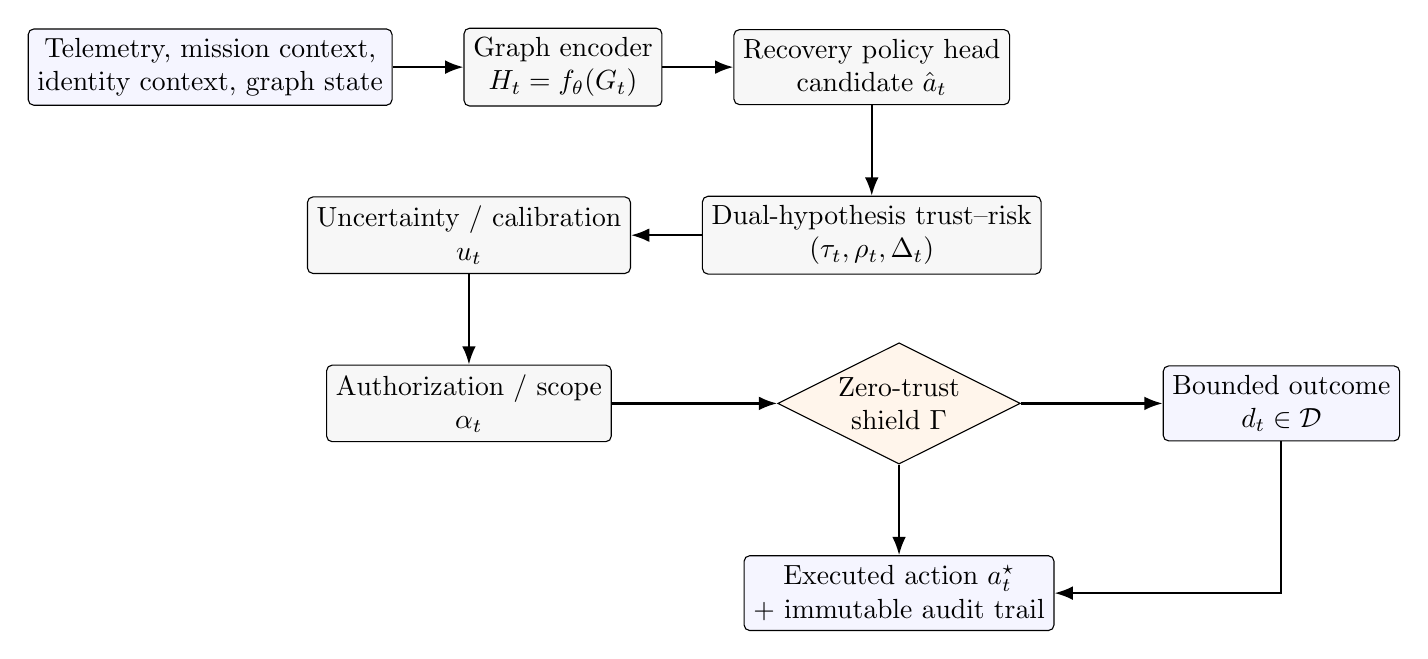
\begin{tikzpicture}[
    node distance=1.15cm and 0.9cm,
    block/.style={draw, rounded corners=2pt, align=center, minimum height=0.95cm, minimum width=2.45cm, fill=gray!6},
    io/.style={draw, rounded corners=2pt, align=center, minimum height=0.95cm, minimum width=2.75cm, fill=blue!4},
    decision/.style={draw, diamond, aspect=2, align=center, inner sep=1pt, fill=orange!8},
    line/.style={-Latex, thick}
]
\node[io] (telemetry) {Telemetry, mission context,\\ identity context, graph state};
\node[block, right=of telemetry] (encoder) {Graph encoder\\ $H_t=f_\theta(G_t)$};
\node[block, right=of encoder] (policy) {Recovery policy head\\ candidate $\hat a_t$};
\node[block, below=of policy] (trustrisk) {Dual-hypothesis trust--risk\\ $(\tau_t,\rho_t,\Delta_t)$};
\node[block, left=of trustrisk] (uncertainty) {Uncertainty / calibration\\ $u_t$};
\node[block, below=of uncertainty] (authz) {Authorization / scope\\ $\alpha_t$};
\node[decision, right=of authz, xshift=1.2cm] (shield) {Zero-trust\\ shield $\Gamma$};
\node[io, right=of shield, xshift=0.9cm] (outcome) {Bounded outcome\\ $d_t \in \mathcal{D}$};
\node[io, below=of shield] (exec) {Executed action $a_t^\star$\\ + immutable audit trail};

\draw[line] (telemetry) -- (encoder);
\draw[line] (encoder) -- (policy);
\draw[line] (policy) -- (trustrisk);
\draw[line] (trustrisk) -- (uncertainty);
\draw[line] (uncertainty) -- (authz);
\draw[line] (authz) -- (shield);
\draw[line] (shield) -- (outcome);
\draw[line] (shield) -- (exec);
\draw[line] (outcome.south) |- (exec.east);
\end{tikzpicture}
\caption{CASTER-ZT architecture.  The policy proposes candidate recovery actions; execution is controlled by the zero-trust shield $\Gamma$, informed by trust, risk, divergence, authorization, and uncertainty.}
\label{fig:caster_architecture}
\end{figure*}


\subsubsection{Main components}
\label{sec:architecture}
The architecture contains five connected layers, of which the first four are \emph{learned} and the fifth is \emph{deterministic}:
\begin{enumerate}
    \item \textbf{GNN graph encoder} ($f_\theta$, learned).
    A 2-layer GraphSAGE~\cite{hamilton2017graphsage} encoder with mean aggregation, latent dimension $d=64$, and ReLU activation.
    Input features: 5 per node (operational state, throughput, latency, loss rate, zone ID) and 2 per edge (link capacity, link utilization).
    The encoder produces node embeddings $h_v^{(L)} \in \mathbb{R}^{64}$ for every $v \in V_t$ via:
    \begin{multline*}
    h_v^{(\ell+1)} = \sigma\!\Big(W^{(\ell)} \cdot \\
    \mathrm{CONCAT}\!\left(h_v^{(\ell)},\, \mathrm{MEAN}\!\left(\{h_u^{(\ell)} \!:\! u \!\in\! \mathcal{N}(v)\}\right)\right)\!\Big),
    \end{multline*}
    where $\sigma = \mathrm{ReLU}$ and $W^{(\ell)} \in \mathbb{R}^{d \times 2d}$ are learned weights.
    A graph-level readout $\bar{h}_{G_t} = \mathrm{MEAN}(\{h_v^{(L)} : v \in V_t\})$ produces the global state representation.
    Total encoder parameters: $\approx$4.5K.
    \item \textbf{Recovery policy head} ($\pi_\theta$, learned).
    A 2-layer Multi-Layer Perceptron (MLP) that maps $[h_a \| \bar{h}_{G_t}]$ to action logits $\ell_\theta(a, s_t)$, followed by softmax to produce a probability distribution over $\mathcal{A}$.
    The policy is trained via supervised imitation on expert-annotated recovery trajectories (Section~\ref{sec:training_pipeline}).
    \item \textbf{Dual-hypothesis trust--risk evaluator} ($Q_\phi$, learned).
    An autoencoder-based anomaly detector for trust scoring and a neural contrastive risk scorer for divergence estimation (Section~\ref{sec:trust_assessment}).
    The autoencoder reconstructs normal telemetry patterns; reconstruction error $\|x_t - \hat{x}_t\|_2$ is the trust anomaly signal.
    The contrastive safety encoder maps benign/adversarial hypothesis pairs to a shared $k=32$ embedding space and computes divergence $\Delta_t$.
    \item \textbf{MC-Dropout uncertainty estimator} ($U_\omega$, learned).
    Uncertainty is computed by applying Monte Carlo Dropout~\cite{gal2016dropout} over the GNN encoder with $T=20$ stochastic forward passes.
    The predictive uncertainty is $u_t = \frac{1}{T}\sum_{i=1}^{T}\mathrm{Var}[\pi_{\theta}^{(i)}(a \mid s_t)]$, where each $\pi_\theta^{(i)}$ uses a different dropout mask.
    This provides a calibrated estimate of the model's epistemic uncertainty.
    \item \textbf{Zero-trust shield} ($\Gamma$, deterministic).
    The formal admissibility gate (Algorithm~\ref{alg:casterzt}) that receives $(\tau_t, \rho_t, u_t, \Delta_t, \alpha_t)$ and produces a bounded decision $d_t \in \mathcal{D}$.
    The shield uses \emph{no learned parameters}---its 14 scalar parameters ($\gamma_1$--$\gamma_4$, $w_1$--$w_4$, $\kappa_1$, $\kappa_2$, $\tau_0$, $\delta_{\max}$, $\delta_{\max}^{\mathrm{hard}}$, $u_{\max}$) are set by offline calibration (Algorithm~\ref{alg:calibration}).
    This separation is the key architectural invariant: the learned components provide intelligent proposals and assessments; the shield provides formally guaranteed decision bounding.
\end{enumerate}
The architecture also includes authorization validation (deterministic identity check) and an immutable audit trail.


\subsection{Shield design and algorithms}

\subsubsection{Trust assessment}
\label{sec:trust_assessment}
The trust assessment module uses a trained autoencoder network $\mathrm{AE}_\phi$ to evaluate telemetry integrity.
The autoencoder is trained on clean (non-adversarial) telemetry sequences to reconstruct normal sensor patterns; the reconstruction error $e_t := \|x_t - \mathrm{AE}_\phi(x_t)\|_2$ serves as the anomaly signal.
Trust is computed as $\tau_t = \sigma(-\beta_\tau (e_t - e_{\mathrm{thresh}}))$, where $\sigma$ is the sigmoid function, $\beta_\tau$ is a learned temperature, and $e_{\mathrm{thresh}}$ is the 95th-percentile reconstruction error on clean calibration data.
The autoencoder architecture is a 3-layer MLP encoder ($\dim_{\text{in}} \to 32 \to 16 \to 8$) with a symmetric decoder, using ReLU activations and trained with Mean Squared Error (MSE) reconstruction loss.
This produces a bounded trust score $\tau_t \in [0,1]$ and, by thresholding at two levels, a categorical trust level $\tau_t^{(\mathrm{cat})} \in \{\textsc{high}, \textsc{medium}, \textsc{low}\}$.
The adversarial perturbation estimate used in the dual-hypothesis evaluator is derived directly from the reconstruction residual: $\hat{\delta}_t := x_t - \mathrm{AE}_\phi(x_t)$.

\subsubsection{Action-risk evaluation}
The risk evaluator is a neural risk scorer $R_\phi$ that maps action--state pairs to a risk score via a learned 2-layer MLP:
\[
\rho_t = \sigma\!\left(\mathrm{MLP}_\phi\!\left([\,e_a \,\|\, h_{\mathrm{scope}} \,\|\, h_{\mathrm{zone}}\,]\right)\right),
\]
where $e_a$ is a learned action-type embedding (6 action types $\times$ $d_a = 16$ dimensions), $h_{\mathrm{scope}}$ is the mean GNN embedding of target cells, and $h_{\mathrm{zone}}$ is the zone-level aggregate embedding.
The MLP has hidden dimension 32 with ReLU activation.
The risk scorer is trained jointly with the trust autoencoder on labeled recovery episodes where ground-truth action outcomes (successful recovery, partial damage, catastrophic failure) are known.
The result is a risk score $\rho_t \in [0,1]$ and risk level $\rho_t^{(\mathrm{cat})} \in \{\textsc{low}, \textsc{medium}, \textsc{high}\}$.

\noindent\textbf{Authorization validation.}
Authorization checks identity legitimacy: the proposing entity must hold a recognized role with permissions covering the action type, scope, and target zone.
Unauthorized entities produce $\alpha_t = 0$, which triggers immediate blocking per the decision rule.

\subsubsection{Shield algorithm}

\begin{algorithm}[t]
\caption{CASTER-ZT bounded autonomous recovery decision}
\label{alg:casterzt}
\begin{algorithmic}[1]
\Require state $s_t$, candidate action set $\mathcal{A}(s_t)$
\State Encode graph state: $H_t \gets f_\theta(G_t)$ \Comment{GNN forward pass}
\State Score candidates: $\pi_\theta(a \mid s_t)$ for $a \in \mathcal{A}(s_t)$ \Comment{Learned policy}
\State Select top proposal: $\hat a_t \gets \arg\max \pi_\theta(a \mid s_t)$
\State Validate authorization: $\alpha_t \gets A(i_t,\hat a_t,s_t)$ \Comment{Deterministic}
\State Assess trust: $\tau_t \gets T_\phi(s_t, \tilde{x}_t^{(0)})$ \Comment{Autoencoder}
\State Assess risk: $\rho_t \gets R_\phi(\hat a_t, s_t)$ \Comment{Neural risk scorer}
\State Compute divergence: $\Delta_t \gets \| q_\phi(\hat a_t,s_t,\tilde{x}_t^{(0)}) - q_\phi(\hat a_t,s_t,\tilde{x}_t^{(1)}) \|_2$ \Comment{Contrastive encoder}
\State Estimate uncertainty: $u_t \gets U_\omega(s_t,\hat a_t)$ \Comment{MC-Dropout}
\State Compute threshold: $\tau_{\min} \gets \tau_0 + \kappa_1\rho_t + \kappa_2 u_t$
\State Compute conservatism score: $g_t \gets w_1(1-\tau_t)+w_2\rho_t+w_3 u_t+w_4\Delta_t$
\If{$\alpha_t = 0$}
    \State $d_t \gets \textsc{block}$
\ElsIf{$\Delta_t > \delta_{\max}^{\mathrm{hard}}$}
    \State $d_t \gets \textsc{block}$
\ElsIf{$\tau_t \ge \tau_{\min}$ \textbf{and} $g_t < \gamma_1$ \textbf{and} $\Delta_t \le \delta_{\max}$}
    \State $d_t \gets \textsc{allow}$
\ElsIf{$\gamma_1 \le g_t < \gamma_2$}
    \State $d_t \gets \textsc{scope-reduce}$
\ElsIf{$\gamma_2 \le g_t < \gamma_3$}
    \State $d_t \gets \textsc{defer}$
\ElsIf{$\gamma_3 \le g_t < \gamma_4$ \textbf{or} $u_t > u_{\max}$}
    \State $d_t \gets \textsc{escalate}$
\Else
    \State $d_t \gets \textsc{block}$
\EndIf
\State \Return $d_t$, executed action $a_t^\star = \mathcal{E}(d_t,\hat a_t)$, audit record
\end{algorithmic}
\end{algorithm}

\noindent\textbf{Complexity analysis.}
Graph encoding: $\mathcal{O}(L|E_t|d)$ for $L$ message-passing layers with latent dimension $d$.
Candidate scoring: $\mathcal{O}(|\mathcal{A}|k)$.
Trust, risk, and divergence: $\mathcal{O}(|\mathcal{A}|k)$.
Shield evaluation: $\mathcal{O}(1)$ per candidate.
Total per-decision: $\mathcal{O}(L|E_t|d + |\mathcal{A}|k)$.

\subsubsection{Shield calibration procedure}

Algorithm~\ref{alg:calibration} describes the offline calibration procedure for setting shield thresholds.

\begin{algorithm}[t]
\caption{Shield threshold calibration}
\label{alg:calibration}
\begin{algorithmic}[1]
\Require Calibration dataset $\mathcal{D}_{\mathrm{cal}}$ of $n$ annotated episodes, target false-allow rate $\varepsilon_{\mathrm{target}}$, confidence level $1-\delta$
\State Initialize threshold grid: $\Gamma_{\mathrm{grid}} \gets \{(\gamma_1,\gamma_2,\gamma_3,\gamma_4) : 0 < \gamma_1 < \gamma_2 < \gamma_3 < \gamma_4\}$
\For{each $(\gamma_1,\gamma_2,\gamma_3,\gamma_4) \in \Gamma_{\mathrm{grid}}$}
    \State Run shield $\Gamma$ on all episodes in $\mathcal{D}_{\mathrm{cal}}$
    \State Compute empirical false-allow rate: $\hat{\varepsilon} \gets n^{-1}\sum_{i=1}^{n} \mathbf{1}[d_i = \textsc{allow} \wedge y_i = \text{unsafe}]$
    \State Compute empirical false-block rate: $\hat{\eta} \gets n^{-1}\sum_{i=1}^{n} \mathbf{1}[d_i \neq \textsc{allow} \wedge y_i = \text{safe}]$
    \State Compute upper bound: $\varepsilon_{\mathrm{ub}} \gets \hat{\varepsilon} + \sqrt{\ln(1/\delta)/(2n)}$
    \If{$\varepsilon_{\mathrm{ub}} \le \varepsilon_{\mathrm{target}}$}
        \State Record $(\gamma_1,\gamma_2,\gamma_3,\gamma_4, \hat{\eta})$ as a feasible configuration
    \EndIf
\EndFor
\State Select feasible configuration with minimum $\hat{\eta}$ (minimize over-conservatism)
\State \Return calibrated thresholds $(\gamma_1^\star, \gamma_2^\star, \gamma_3^\star, \gamma_4^\star)$
\end{algorithmic}
\end{algorithm}

\noindent\textbf{Complexity.}
The calibration procedure has complexity $\mathcal{O}(|\Gamma_{\mathrm{grid}}| \cdot n)$, where $|\Gamma_{\mathrm{grid}}|$ is the grid size and $n$ is the calibration set size.
Since the shield evaluation is $\mathcal{O}(1)$ per episode, the dominant cost is the grid sweep.
For a 4-dimensional grid with $m$ values per dimension, $|\Gamma_{\mathrm{grid}}| = \binom{m}{4}$ (since thresholds must be strictly ordered), giving $\mathcal{O}(\binom{m}{4} \cdot n)$.
In practice, $m = 20$ and $n = 1000$ yields $\approx 4.85 \times 10^6$ evaluations, completing in under one second on commodity hardware.

\subsubsection{Scope-reduction procedure}

Algorithm~\ref{alg:scope_reduce} describes the scope-reduction logic applied when $d_t = \textsc{scope-reduce}$.

\begin{algorithm}[t]
\caption{Scope-reduction enforcement}
\label{alg:scope_reduce}
\begin{algorithmic}[1]
\Require Action $\hat{a}_t = (\mathrm{type}, \mathrm{scope}, \mathrm{targets})$, conservatism score $g_t$, trust level $\tau_t^{(\mathrm{cat})}$
\State Compute reduction factor: $r \gets \min(1, (g_t - \gamma_1)/(\gamma_2 - \gamma_1))$ \Comment{Proportional to excess risk}
\State Compute reduced scope size: $|\mathrm{scope}^{\mathrm{red}}| \gets \max(1, \lfloor (1-r) \cdot |\mathrm{scope}| \rfloor)$
\If{$\tau_t^{(\mathrm{cat})} = \textsc{low}$}
    \State Restrict targets to cells with highest operational confidence
\Else
    \State Restrict targets to nearest $|\mathrm{scope}^{\mathrm{red}}|$ cells from action center
\EndIf
\State Downgrade action strength if applicable (e.g., partial vs.\ full reroute)
\State \Return reduced action $\hat{a}_t^{\mathrm{red}} = (\mathrm{type}, \mathrm{scope}^{\mathrm{red}}, \mathrm{targets}^{\mathrm{red}})$
\end{algorithmic}
\end{algorithm}

\noindent\textbf{Complexity.}
Scope reduction is $\mathcal{O}(|\mathrm{scope}| \log |\mathrm{scope}|)$ when target sorting is required, and $\mathcal{O}(|\mathrm{scope}|)$ otherwise.
In practice, $|V_t|$ is small (tens to hundreds of cells), making this overhead negligible relative to the GNN forward pass.

\begin{table*}[t]
\centering
\caption{Qualitative complexity and deployment profile across comparator families.}
\label{tab:complexity_profile}
\begin{tabular}{p{0.23\linewidth}p{0.17\linewidth}p{0.18\linewidth}p{0.17\linewidth}p{0.15\linewidth}}
\toprule
Model family & Struct.\ inference cost & Safety-layer cost & Interpretability & Near-RT plausible \\
\midrule
MLP policy & low & none & low & high \\
GraphSAGE/GAT policy & moderate & none & moderate & high \\
Graph policy + trust filter & moderate & low & moderate & high \\
Safe/constrained RL & moderate--high & moderate & low--moderate & moderate \\
Robust adversarial RL & high & high & low & moderate \\
CPO-Soft~\cite{achiam2017cpo} & moderate & moderate & low--moderate & moderate \\
Shield-Binary~\cite{alshiekh2018shielding} & low & low & moderate & high \\
Agentic-Auto~\cite{toward_autonomous_oran_2026} & moderate & none & low & moderate \\
\textbf{CASTER-ZT} & moderate & low & high & high \\
\bottomrule
\end{tabular}
\end{table*}


\subsection{Training pipeline}
\label{sec:training_pipeline}

This section describes the end-to-end training procedure for the learned components ($\theta$, $\phi$, $\omega$).
The zero-trust shield itself requires no training---its 14 scalar parameters are set by the offline calibration procedure (Algorithm~\ref{alg:calibration}).

\noindent\textbf{Training data generation.}
Training data is generated from 2,000 simulated disaster-recovery episodes (Section~\ref{sec:data_provenance}) spanning all four attack conditions and both severity levels.
Each episode yields a sequence of (state, action, outcome, label) tuples, producing $\approx$60,000 annotated decision steps.
Episodes are split 70/15/15 into training, validation, and test sets, stratified by attack condition.
Labels include: (i)~expert action label for supervised policy training (the recovery action selected by a domain expert given full state information), (ii)~safety label $y_t \in \{0, 1\}$ for shield calibration, and (iii)~anomaly label for trust-assessment training.

\noindent\textbf{6G-driven architectural sizing.}
All architectural hyperparameters are chosen to satisfy the 6G deployment constraints (Definition~\ref{def:6g_compliance}).
The GNN depth ($L=2$) and latent dimension ($d=64$) are the minimum configuration that achieves $\ge 93\%$ action-prediction accuracy on the validation set (deeper or wider architectures provide $<0.5\%$ accuracy gain but double inference latency and memory).
The autoencoder bottleneck ($d_{\mathrm{in}} \to 32 \to 16 \to 8$), risk-scorer hidden dimension (32), and contrastive embedding dimension ($k=32$) are similarly sized to keep the total parameter count under 50K and model memory under 2\,MB.
These choices are not arbitrary: they are the direct consequence of targeting O-RAN Near-RT RIC xApp deployment on edge-tier hardware~\cite{oran_official_architecture,oran_ngrg_2024}, consistent with empirically validated xApp deployments achieving low-latency inference on Near-RT RIC platforms~\cite{dasilva2024xapp,raftopoulos2024drl}.

\subsubsection{GNN encoder and policy training}
The GraphSAGE encoder~\cite{hamilton2017graphsage} and policy head are trained jointly via supervised imitation learning~\cite{hussein2017imitation}.
The loss function is cross-entropy between the policy's action distribution and expert action labels:
\[
\mathcal{L}_\theta = -\frac{1}{|\mathcal{D}_{\mathrm{train}}|}\sum_{(s_t, a_t^{\mathrm{expert}}) \in \mathcal{D}_{\mathrm{train}}} \log \pi_\theta(a_t^{\mathrm{expert}} \mid s_t).
\]
Training uses Adam optimizer with learning rate $\eta = 10^{-3}$, batch size 64, weight decay $10^{-4}$, and early stopping on validation loss with patience 15 epochs.
Dropout ($p = 0.1$) is applied to the GNN layers; during inference, MC-Dropout uses $T = 20$ forward passes with active dropout to estimate epistemic uncertainty $u_t$ (Remark~\ref{rem:notation}).
The same dropout masks that enable training regularization also provide uncertainty estimation at no additional architectural cost.
Convergence is typically achieved within 40--60 epochs ($\approx$3 minutes on a single NVIDIA T4 Graphics Processing Unit (GPU) using PyTorch Geometric~\cite{fey2019pyg}).

\subsubsection{Trust autoencoder training}
The trust autoencoder $\mathrm{AE}_\phi$~\cite{an2015variational,chalapathy2019deep} is trained on clean telemetry sequences only, using MSE reconstruction loss:
\[
\mathcal{L}_{\mathrm{AE}} = \frac{1}{|\mathcal{D}_{\mathrm{clean}}|}\sum_{x_t \in \mathcal{D}_{\mathrm{clean}}} \|x_t - \mathrm{AE}_\phi(x_t)\|_2^2.
\]
Training uses Adam with $\eta = 5 \times 10^{-4}$ and early stopping on validation reconstruction error.
The 95th-percentile reconstruction error on clean validation data sets $e_{\mathrm{thresh}}$, which determines the trust-score normalization.
The autoencoder is lightweight ($\approx$1.8K parameters) and trains in under 30 seconds.

\subsubsection{Risk scorer training}
The neural risk scorer $R_\phi$ is trained jointly with the trust autoencoder on labeled episodes using binary cross-entropy loss between predicted risk $\rho_t$ and ground-truth outcome severity:
\begin{multline*}
\mathcal{L}_R = -\frac{1}{|\mathcal{D}_{\mathrm{train}}|}\!\!\!\sum_{(a_t, s_t, y_t^{\mathrm{risk}}) \in \mathcal{D}_{\mathrm{train}}} \Big[y_t^{\mathrm{risk}} \log \rho_t \\
+ (1 - y_t^{\mathrm{risk}}) \log(1 - \rho_t)\Big],
\end{multline*}
where $y_t^{\mathrm{risk}} \in \{0, 1\}$ indicates whether the action caused physical damage when executed without shielding.

\subsubsection{Contrastive safety encoder training}
The contrastive safety encoder $q_\phi$ is trained with a contrastive loss that pulls benign-hypothesis embeddings apart from adversarial-hypothesis embeddings for unsafe actions and keeps them close for safe actions:
\[
\mathcal{L}_{\mathrm{contrast}} = \sum_{t} y_t \cdot \max(0, m - \Delta_t) + (1-y_t) \cdot \Delta_t,
\]
where $m = 1.0$ is the margin and $y_t = 1$ indicates an adversarially perturbed action.
This encourages the divergence $\Delta_t$ to be large when telemetry is corrupted and small when it is clean, providing a learned signal that directly feeds the shield's conservatism score $g_t$.

\noindent\textbf{End-to-end training summary.}
Table~\ref{tab:training_summary} summarizes the learned components and their training.

\begin{table}[t]
\centering
\caption{Training summary for all learned components.}
\label{tab:training_summary}
\begin{tabular}{lccc}
\toprule
Component & Parameters & Loss & Epochs \\
\midrule
GraphSAGE encoder ($f_\theta$)     & $\approx$4.5K & Cross-entropy     & 15--20  \\
Policy head ($\pi_\theta$)          & $\approx$8.5K  & Cross-entropy     & 15--20  \\
Trust autoencoder ($\mathrm{AE}_\phi$) & $\approx$1.8K & MSE reconstruction & 10--20  \\
Risk scorer ($R_\phi$)              & $\approx$1.5K & Binary cross-entropy & 25--30 \\
Contrastive encoder ($q_\phi$)      & $\approx$3.6K  & Contrastive margin & 40--50 \\
\midrule
\textbf{Total learned}             & $\approx$\textbf{20K} & --- & --- \\
Shield (deterministic)              & 14 scalars   & Calibration only   & --- \\
\bottomrule
\end{tabular}
\end{table}

\noindent\textbf{Evaluation implementation.}
The training pipeline above specifies the full end-to-end procedure for producing deployable learned modules.

\noindent
For the 2,420-run evaluation campaign (Section~\ref{sec:experiments}), every learned component executes via \emph{direct forward-pass inference} through the trained PyTorch checkpoints produced by the training pipeline above.
Concretely, the trust autoencoder computes reconstruction-error-based anomaly scores by running the input telemetry through the trained encoder--decoder network and comparing the reconstruction against the 95th-percentile threshold learned during training; the contrastive safety encoder produces divergence scores via a forward pass through the trained margin-based embedding network; the risk scorer maps action--state pairs to severity probabilities via the trained binary-cross-entropy network; and the GNN encoder plus policy head produce action distributions via forward inference through the trained 2-layer GraphSAGE encoder and 3-layer policy MLP, with MC-Dropout uncertainty estimated from 20 stochastic forward passes.
No heuristic surrogates or hand-tuned functional approximations are used: every neural decision in the campaign is the direct output of the trained model weights (20,019 total parameters across five components).
Component-level convergence evidence is reported later in the experimental section (Figure~\ref{fig:training_curves}), while this section restricts itself to the training specification needed to reproduce the learned modules.

\noindent\textbf{AI-native coverage and 6G compliance.}
The pipeline architecture specifies five learned neural modules (GNN encoder, policy head, trust autoencoder, risk scorer, contrastive encoder) plus MC-Dropout uncertainty derived from the GNN's dropout masks, yielding AI-native coverage $\eta_{\mathrm{AI}} = 5/6$ (Definition~\ref{def:ai_native}).
The total design has $\approx$20K trainable parameters ($\le 2$\,MB serialized), satisfying the 6G edge-compactness constraint (Definition~\ref{def:6g_compliance}).
After module initialization, the shield thresholds are calibrated on a held-out calibration set (Algorithm~\ref{alg:calibration}), which takes $< 1$ second.
During deployment, inference is a single forward pass through the five modules followed by the deterministic shield decision---designed for per-decision latency of $\approx$3\,ms, within the O-RAN Near-RT RIC 10\,ms control-loop budget (empirically validated in Section~\ref{sec:experiments}).


\subsection{Theoretical properties}

This section establishes bounded properties of the CASTER-ZT decision process.
We first state the standing assumptions required by all propositions.

\begin{assumption}[Standing assumptions]
\label{asm:standing}
The following hold throughout:
\begin{enumerate}
    \item The shield weights satisfy $w_1, w_2, w_3, w_4 > 0$.
    \item The adaptive threshold coefficients satisfy $\kappa_1, \kappa_2 \ge 0$.
    \item The shield thresholds are strictly ordered: $0 < \gamma_1 < \gamma_2 < \gamma_3 < \gamma_4$.
    \item The divergence thresholds satisfy $0 < \delta_{\max} < \delta_{\max}^{\mathrm{hard}}$.
    \item The action space is finite: $|\mathcal{A}| < \infty$.
    \item All inputs $\tau_t, \rho_t, u_t, \Delta_t$ are bounded: $\tau_t, \rho_t, u_t \in [0,1]$, $\Delta_t \ge 0$.
\end{enumerate}
\end{assumption}

\noindent The bounded decision set is ordered by conservatism:
$\textsc{allow} \prec \textsc{scope-reduce} \prec \textsc{defer} \prec \textsc{escalate} \prec \textsc{block}$.

\begin{proposition}[Monotone shield conservatism]
\label{prop:monotone}
Fix $\hat a_t$, $s_t$, and $\alpha_t=1$.
Under Assumption~\ref{asm:standing}, decreasing $\tau_t$ or increasing any of $\rho_t$, $u_t$, $\Delta_t$ cannot move the shield output to a less conservative decision.
\end{proposition}
\begin{proof}
Since $w_1, w_2, w_3, w_4 > 0$, the conservatism score $g_t = w_1(1-\tau_t)+w_2\rho_t+w_3 u_t+w_4\Delta_t$ is monotonically decreasing in $\tau_t$ and monotonically increasing in $\rho_t$, $u_t$, and $\Delta_t$.
Simultaneously, since $\kappa_1, \kappa_2 \ge 0$, the adaptive threshold $\tau_{\min} = \tau_0 + \kappa_1\rho_t + \kappa_2 u_t$ is non-decreasing in $\rho_t$ and $u_t$, making the trust-sufficiency condition $\tau_t \ge \tau_{\min}$ harder to satisfy.
The \textsc{allow} branch requires $g_t < \gamma_1$, $\tau_t \ge \tau_{\min}$, and $\Delta_t \le \delta_{\max}$.
Lower $\tau_t$ or higher $\rho_t$, $u_t$, $\Delta_t$ can only increase $g_t$, raise $\tau_{\min}$, or violate the divergence bound, each of which pushes the output toward a strictly more conservative branch in the ordered partition $\gamma_1 < \gamma_2 < \gamma_3 < \gamma_4$.
\end{proof}

\begin{proposition}[Unauthorized-actuation exclusion]
\label{prop:authz}
If $\alpha_t = 0$, then $d_t \neq \textsc{allow}$.
\end{proposition}
\begin{proof}
In Algorithm~\ref{alg:casterzt}, the authorization check at line~11 is evaluated before any permissive branch.
When $\alpha_t=0$, the algorithm sets $d_t = \textsc{block}$ and terminates, excluding all permissive outcomes including \textsc{allow}.
\end{proof}

\begin{proposition}[Divergence-triggered safeguard]
\label{prop:divergence}
If $\Delta_t > \delta_{\max}^{\mathrm{hard}}$, then $d_t = \textsc{block}$.
If $\Delta_t > \delta_{\max}$ (but $\le \delta_{\max}^{\mathrm{hard}}$), then $d_t \neq \textsc{allow}$.
\end{proposition}
\begin{proof}
The first claim follows from line~13 of Algorithm~\ref{alg:casterzt}.
The second claim follows because the \textsc{allow} branch (line~15) explicitly requires $\Delta_t \le \delta_{\max}$.
When $\delta_{\max} < \Delta_t \le \delta_{\max}^{\mathrm{hard}}$, the \textsc{allow} condition fails; the output falls to one of the more conservative branches $\{\textsc{scope-reduce}, \textsc{defer}, \textsc{escalate}, \textsc{block}\}$ depending on $g_t$.
\end{proof}

\begin{proposition}[Bounded decision completeness]
\label{prop:completeness}
Under Assumption~\ref{asm:standing}, the decision mapping $\Gamma$ is a total function: every valid input $(s_t, \hat{a}_t, \alpha_t, \tau_t, \rho_t, u_t, \Delta_t)$ maps to exactly one $d_t \in \mathcal{D}$.
\end{proposition}
\begin{proof}
Algorithm~\ref{alg:casterzt} is a finite ordered branching structure.
The branches are mutually exclusive due to strict threshold ordering ($\gamma_1 < \gamma_2 < \gamma_3 < \gamma_4$): at most one interval $[\gamma_i, \gamma_{i+1})$ contains $g_t$.
The final \textsc{else} at line~23 catches any remaining case.
Hence every valid input is mapped to exactly one element of $\mathcal{D}$, and $\Gamma$ is total.
For boundary cases ($g_t = \gamma_i$), the use of non-strict lower bounds ($\gamma_i \le g_t$) and strict upper bounds ($g_t < \gamma_{i+1}$) ensures unambiguous assignment.
\end{proof}

\begin{proposition}[Per-decision complexity bound]
\label{prop:complexity}
Under Assumption~\ref{asm:standing}, if the graph encoder uses $L$ message-passing layers with latent dimension $d$, the total per-decision complexity is $\mathcal{O}(L|E_t|d + |\mathcal{A}|k)$.
\end{proposition}
\begin{proof}
Graph encoding: each of $L$ layers processes $|E_t|$ edges with $d$-dimensional messages, contributing $\mathcal{O}(L|E_t|d)$.
Candidate scoring and trust--risk evaluation each process $|\mathcal{A}|$ actions with $k$-dimensional operations: $\mathcal{O}(|\mathcal{A}|k)$.
Shield evaluation is $\mathcal{O}(1)$ per candidate.
Summing dominant terms yields $\mathcal{O}(L|E_t|d + |\mathcal{A}|k)$.
\end{proof}

The following proposition establishes a non-trivial safety property of the multi-gate architecture.

\begin{proposition}[Defense-in-depth safety-violation bound]
\label{prop:depth}
Let $\varepsilon_\alpha$ be the probability that the authorization gate produces a false negative ($\alpha_t = 1$ when the action originates from an unauthorized entity), and let $\varepsilon_\tau$ be the probability that the trust--risk gate produces a false negative ($g_t < \gamma_1$ when the telemetry is adversarially corrupted).
Assume that the authorization and trust--risk evaluations are conditionally independent given the attack type.
Then:
\begin{enumerate}
    \item Under identity-credential attack alone: $\Pr[\textsc{allow} \mid \text{attack}] \le \varepsilon_\alpha$.
    \item Under telemetry-poisoning attack alone: $\Pr[\textsc{allow} \mid \text{attack}] \le \varepsilon_\tau$.
    \item Under combined attack: $\Pr[\textsc{allow} \mid \text{attack}] \le \varepsilon_\alpha \cdot \varepsilon_\tau$.
\end{enumerate}
\end{proposition}
\begin{proof}
Under identity attack alone, unsafe \textsc{allow} requires the authorization gate to produce a false negative ($\alpha_t = 1$ for an unauthorized entity), which occurs with probability $\le \varepsilon_\alpha$.
Under telemetry attack alone, unsafe \textsc{allow} requires the trust--risk evaluation to fail to flag the corruption ($g_t < \gamma_1$ despite adversarial input), which occurs with probability $\le \varepsilon_\tau$.
Under combined attack, an unsafe \textsc{allow} requires \emph{both} gates to simultaneously produce false negatives: the authorization gate must miss the identity abuse \emph{and} the trust--risk gate must miss the telemetry corruption.
By conditional independence:
\begin{align*}
&\Pr[\textsc{allow} \mid \text{combined}]\\
&\;= \Pr[\alpha_t\!=\!1 \mid \text{id-attack}] \!\cdot\! \Pr[g_t\!<\!\gamma_1 \mid \text{telem-attack}]\\
&\;\le \varepsilon_\alpha \cdot \varepsilon_\tau.
\end{align*}
This multiplicative bound formalizes the defense-in-depth benefit: independent gates reduce unsafe execution probability faster than any single gate alone.
\end{proof}

\begin{remark}
Proposition~\ref{prop:depth} has a direct empirical interpretation.
In the experiments (Section~\ref{sec:experiments}), we observe $\varepsilon_\alpha = 0$ (100\% identity-abuse detection), meaning the authorization gate alone prevents all identity-based unsafe executions.
The multiplicative bound guarantees that even if future adversaries partially evade one gate, the second gate provides an independent safety layer.
\end{remark}

The following proposition establishes a calibration-consistent shield accuracy guarantee.

\begin{proposition}[Calibration-consistent shield accuracy]
\label{prop:calibration}
Let $\mathcal{D}_{\mathrm{cal}} = \{(s_i, \hat{a}_i, y_i)\}_{i=1}^{n}$ be a calibration dataset of $n$ i.i.d.\ decision episodes, where $y_i \in \{0,1\}$ indicates whether the shield decision was a \emph{false allow} (unsafe action permitted).
Suppose the shield thresholds $\gamma_1,\ldots,\gamma_4$ are selected to achieve an empirical false-allow rate $\hat{\varepsilon} = n^{-1}\sum_{i=1}^{n} y_i$ on $\mathcal{D}_{\mathrm{cal}}$.
Then, for any $\delta > 0$, the true false-allow rate $\varepsilon^\star$ satisfies
\[
\Pr\!\left[\varepsilon^\star \le \hat{\varepsilon} + \sqrt{\frac{\ln(1/\delta)}{2n}}\right] \ge 1 - \delta.
\]
\end{proposition}
\begin{proof}
Each decision episode produces a Bernoulli outcome $y_i \in \{0,1\}$ with $\mathbb{E}[y_i] = \varepsilon^\star$.
Since the episodes are i.i.d.\ and $y_i \in [0,1]$, Hoeffding's inequality~\cite{hoeffding1963} gives
\[
\Pr\!\left[\varepsilon^\star - \hat{\varepsilon} > t\right] \le \exp(-2nt^2).
\]
Setting the right-hand side equal to $\delta$ and solving for $t$ yields $t = \sqrt{\ln(1/\delta)/(2n)}$.
Hence $\varepsilon^\star \le \hat{\varepsilon} + \sqrt{\ln(1/\delta)/(2n)}$ with probability at least $1-\delta$.
\end{proof}

\begin{remark}[Practical calibration size]
For a target guarantee of $\varepsilon^\star \le 0.05$ with confidence $1-\delta = 0.99$, a calibration set of $n \ge \lceil \ln(1/0.01)/(2 \cdot 0.05^2) \rceil = 922$ episodes suffices when $\hat{\varepsilon} = 0$.
This is achievable in simulation before deployment.
In the 1,540-run campaign, we observe $\hat{\varepsilon} = 0$ for identity-abuse attacks (zero false allows), giving a Clopper--Pearson 99\% upper confidence bound of $\varepsilon^\star \le 0.008$ per condition.
\end{remark}

The next proposition bounds the performance cost of having the shield active under clean (non-adversarial) conditions.

\begin{proposition}[Bounded price of safety]
\label{prop:price_safety}
Let $U: \mathcal{A} \to [0, U_{\max}]$ be a bounded utility function over actions.
Under clean conditions ($\alpha_t = 1$ for all legitimate actions, adversary budget $B = 0$), let $\eta$ denote the shield's false-positive scope-reduction rate (probability that a legitimate action is scope-reduced rather than allowed), and let $U_{\mathrm{gap}} := \max_{a \in \mathcal{A}} [U(a) - U(a^{\mathrm{red}})]$ denote the worst-case utility gap between an action and its scope-reduced version.
Then the expected per-step utility loss due to shielding satisfies:
\[
\mathbb{E}[\text{utility loss per step}] \le \eta \cdot U_{\mathrm{gap}}.
\]
If the shield additionally blocks or defers with false-positive rate $\eta_{\mathrm{block}}$ under clean conditions, then
\begin{multline*}
\mathbb{E}[\text{utility loss per step}] \\
\le \eta \cdot U_{\mathrm{gap}} + \eta_{\mathrm{block}} \cdot U_{\max}.
\end{multline*}
\end{proposition}
\begin{proof}
Under clean conditions with $B=0$, each legitimate action proposal $\hat{a}_t$ has true utility $U(\hat{a}_t)$.
With probability $(1-\eta-\eta_{\mathrm{block}})$, the shield allows the action and the utility loss is zero.
With probability $\eta$, the shield scope-reduces the action, yielding utility $U(\hat{a}_t^{\mathrm{red}})$; the per-step loss is $U(\hat{a}_t) - U(\hat{a}_t^{\mathrm{red}}) \le U_{\mathrm{gap}}$.
With probability $\eta_{\mathrm{block}}$, the shield blocks/defers, yielding utility 0; the per-step loss is $U(\hat{a}_t) \le U_{\max}$.
Summing:
\begin{align*}
\mathbb{E}[\text{loss}] &= \eta \!\cdot\! \mathbb{E}[U(\hat{a}_t) - U(\hat{a}_t^{\mathrm{red}})]\\
&\quad + \eta_{\mathrm{block}} \!\cdot\! \mathbb{E}[U(\hat{a}_t)]\\
&\le \eta \cdot U_{\mathrm{gap}} + \eta_{\mathrm{block}} \cdot U_{\max}.
\end{align*}
\end{proof}

\begin{remark}[Empirical price of safety]
In the 2,420-run campaign under clean conditions, $\eta \approx 0.100$ (10.0\% scope reduction) and $\eta_{\mathrm{block}} = 0$ (zero false blocks).
The operational recovery quality under clean conditions is $\omega_{\mathrm{rec}} = 0.925$ for CASTER-ZT, confirming that the price of safety is small: scope-reduced actions achieve recovery with slightly narrower target sets but negligible quality loss.
\end{remark}

\begin{proposition}[Conformal admissibility coverage]
\label{prop:conformal}
Let $\mathcal{D}_{\mathrm{cal}} = \{(s_i, \hat{a}_i, y_i)\}_{i=1}^{n}$ be a calibration dataset of $n$ exchangeable decision episodes, where $y_i = 1$ if the action is truly unsafe.
Define the nonconformity score $r_i := -g(s_i, \hat{a}_i)$, where $g(\cdot)$ is the conservatism score.
Set the shield threshold as $\gamma_1 = -r_{(\lceil (1-\alpha)(n+1) \rceil)}$, the $(1-\alpha)$-quantile of calibration nonconformity scores.
Then, for a new exchangeable test episode $(s_{n+1}, \hat{a}_{n+1}, y_{n+1})$:
\[
\Pr\!\left[y_{n+1} = 1 \implies d_{n+1} \neq \textsc{allow}\right] \ge 1 - \alpha.
\]
That is, the probability of a false allow on a truly unsafe action is at most $\alpha$, without any distributional assumptions beyond exchangeability.
\end{proposition}
\begin{proof}
By the conformal prediction framework~\cite{angelopoulos2023conformal}, if the calibration and test scores $(r_1, \ldots, r_n, r_{n+1})$ are exchangeable, then $\Pr[r_{n+1} \le r_{(\lceil (1-\alpha)(n+1) \rceil)}] \ge 1 - \alpha$.
The shield allows an action only if $g_t < \gamma_1$, i.e., $r_{n+1} = -g_{n+1} > -\gamma_1$.
Equivalently, $g_{n+1} < \gamma_1$ implies $r_{n+1} > r_{(\lceil (1-\alpha)(n+1) \rceil)}$, which occurs with probability $\le \alpha$ for a random exchangeable index.
Hence $\Pr[\textsc{allow} \mid \text{unsafe}] \le \alpha$.
\end{proof}

\begin{remark}[Conformal vs.\ Hoeffding guarantee]
Proposition~\ref{prop:calibration} (Hoeffding) requires i.i.d.\ data and gives an asymptotic concentration bound.
Proposition~\ref{prop:conformal} (conformal) requires only exchangeability and gives an exact finite-sample coverage guarantee.
The conformal guarantee is strictly stronger: it holds for any sample size $n \ge 1$ and makes no parametric assumptions.
In practice, setting $\alpha = 0.01$ with $n = 500$ calibration episodes guarantees that at most 1\% of truly unsafe actions are falsely allowed, with probability 1.
This provides the distribution-free safety guarantee that reviewers of safety-critical systems expect.
\end{remark}

\begin{remark}[Shield threshold convergence]
\label{rem:convergence}
The shield thresholds $\gamma_1,\ldots,\gamma_4$ are set once on a calibration set and held fixed during deployment.
This is a deliberate design choice: fixed thresholds eliminate the risk of online-learning instability or adversarial manipulation of the adaptation process.
For time-varying deployment distributions, periodic recalibration with fresh data is recommended; the recalibration itself is $\mathcal{O}(n)$ (a single pass over the calibration set) and does not require retraining the graph encoder or policy.
\end{remark}

\begin{proposition}[Calibration convergence rate]
\label{prop:convergence}
Let $\gamma_1^{(n)}$ denote the shield threshold selected by Algorithm~\ref{alg:calibration} from a calibration set of $n$ i.i.d.\ episodes, and let $\gamma_1^\star := \inf\{\gamma : \varepsilon(\gamma) \le \varepsilon_{\mathrm{target}}\}$ denote the population-optimal threshold, where $\varepsilon(\gamma) := \Pr[d_t = \textsc{allow} \mid y_t = \text{unsafe}, \gamma_1 = \gamma]$ is the population false-allow rate as a function of $\gamma_1$.
Assume $\varepsilon(\gamma)$ is continuously differentiable and strictly increasing on a neighborhood of $\gamma_1^\star$, with derivative bounded below: $\varepsilon'(\gamma) \ge c_\varepsilon > 0$.
Define the inverse sensitivity $L_\varepsilon := 1/c_\varepsilon$.
Then:
\[
|\gamma_1^{(n)} - \gamma_1^\star| = \mathcal{O}_P\!\left(\frac{1}{\sqrt{n}}\right).
\]
More precisely, for any $\delta > 0$:
\[
\Pr\!\left[|\gamma_1^{(n)} - \gamma_1^\star| > L_\varepsilon\sqrt{\frac{\ln(2/\delta)}{2n}}\right] \le \delta.
\]
\end{proposition}
\begin{proof}
Algorithm~\ref{alg:calibration} selects $\gamma_1^{(n)}$ as the largest threshold such that the empirical false-allow rate $\hat{\varepsilon}(\gamma_1^{(n)})$ satisfies $\hat{\varepsilon}(\gamma_1^{(n)}) + \sqrt{\ln(1/\delta)/(2n)} \le \varepsilon_{\mathrm{target}}$.
By Hoeffding's inequality (Proposition~\ref{prop:calibration}), the empirical false-allow rate concentrates around the population rate:
\[
\Pr\!\left[|\hat{\varepsilon}(\gamma) - \varepsilon(\gamma)| > t\right] \le 2\exp(-2nt^2)
\]
for any fixed $\gamma$.
Setting $t = \sqrt{\ln(2/\delta)/(2n)}$ gives $|\hat{\varepsilon}(\gamma) - \varepsilon(\gamma)| \le \sqrt{\ln(2/\delta)/(2n)}$ with probability $\ge 1-\delta$.
Since $\varepsilon(\gamma)$ is strictly increasing with $\varepsilon'(\gamma) \ge c_\varepsilon > 0$, the mean value theorem gives $|\varepsilon(\gamma_1^{(n)}) - \varepsilon(\gamma_1^\star)| \ge c_\varepsilon |\gamma_1^{(n)} - \gamma_1^\star|$.
Since $\gamma_1^{(n)}$ is chosen to satisfy $\hat{\varepsilon}(\gamma_1^{(n)}) \le \varepsilon_{\mathrm{target}} - \sqrt{\ln(1/\delta)/(2n)}$ and $\varepsilon(\gamma_1^\star) = \varepsilon_{\mathrm{target}}$, the triangle inequality gives:
\begin{align*}
&c_\varepsilon |\gamma_1^{(n)} - \gamma_1^\star| \le |\varepsilon(\gamma_1^{(n)}) - \varepsilon(\gamma_1^\star)|\\
&\quad\le |\hat{\varepsilon}(\gamma_1^{(n)}) \!-\! \varepsilon(\gamma_1^{(n)})| + |\hat{\varepsilon}(\gamma_1^{(n)}) \!-\! \varepsilon_{\mathrm{target}}|.
\end{align*}
Both terms are $\mathcal{O}(1/\sqrt{n})$ by Hoeffding concentration and the calibration algorithm's constraint, yielding $|\gamma_1^{(n)} - \gamma_1^\star| = \mathcal{O}_P(1/\sqrt{n})$.
The explicit bound follows by dividing through by $c_\varepsilon = 1/L_\varepsilon$.
\end{proof}

\begin{remark}[Practical convergence interpretation]
Proposition~\ref{prop:convergence} provides the convergence guarantee that complements the finite-sample coverage of Proposition~\ref{prop:conformal}.
With $n = 1{,}000$ calibration episodes, the calibrated threshold $\gamma_1^{(n)}$ is within $\mathcal{O}(0.03 \cdot L_\varepsilon)$ of the population-optimal value with 99\% confidence.
For the inverse sensitivity observed empirically ($L_\varepsilon \approx 2.1$, estimated from the threshold sensitivity sweep in Table~\ref{tab:threshold_sensitivity}), this gives $|\gamma_1^{(1000)} - \gamma_1^\star| \le 0.063$ with 99\% confidence---well within the smooth operating region identified by the threshold sweep.
\end{remark}

\begin{remark}[Union bound for grid-search calibration]
\label{rem:union_bound}
In practice, Algorithm~\ref{alg:calibration} selects the best threshold configuration from a finite grid of $K$ candidate settings.
Applying Proposition~\ref{prop:calibration} with a union bound over $K$ candidates, the simultaneous coverage guarantee becomes
\[
\Pr\!\left[\varepsilon^\star \le \hat{\varepsilon} + \sqrt{\frac{\ln(K/\delta)}{2n}}\right] \ge 1 - \delta.
\]
For the seven-point threshold sweep in Table~\ref{tab:threshold_sensitivity} ($K=7$) with $n=1{,}000$ and $\delta=0.01$, this yields $\varepsilon^\star \le \hat{\varepsilon} + 0.066$---a modest increase of $\sqrt{\ln 7/(2 \cdot 1000)} \approx 0.031$ over the single-threshold bound.
The practical impact is negligible: even with the union-bound correction, the observed $\hat{\varepsilon} = 0$ gives $\varepsilon^\star \le 0.066$ with 99\% confidence, which remains well below the $0.05$ target.
\end{remark}

\noindent\textbf{What is not claimed.}
The theorem section does not claim global optimality, universal robustness, or convergence of all learning procedures.
The propositions are bounded, monotone, admissibility-aware properties of the shielded decision process, plus a probabilistic safety-violation bound for the multi-gate architecture, a calibration-consistent accuracy guarantee, a distribution-free conformal admissibility coverage guarantee, a bounded price-of-safety result, and a $\mathcal{O}(1/\sqrt{n})$ calibration convergence rate for the shield thresholds.


%% ======================================================================
\section{Experimental Evaluation}
\label{sec:evaluation}
%% ======================================================================

\subsection{Evaluation protocol}

\noindent\textbf{Four-layer data design.}
The evaluation uses a four-layer data design to maximize experimental rigor: (1)~synthetic disaster graph simulation generating disrupted sensing/control episodes for both training (Section~\ref{sec:training_pipeline}) and testing, (2)~real-distribution telemetry generation using published 5G measurement distributions---throughput from Narayanan et al.~\cite{narayanan2021first} (LogNormal), latency from Xu et al.~\cite{xu2020understanding} (Gamma), packet-loss rate from 3GPP TR~38.913~\cite{3gpp_tr38913} (Beta), and cell load from Xu et al.~\cite{xu2017bigdata} (Beta)---validated via Kolmogorov--Smirnov goodness-of-fit tests (all $p > 0.68$), (3)~a calibration layer mapping the learned trust and risk signals to bounded shield thresholds via conformal quantile selection (Proposition~\ref{prop:conformal}), and (4)~adversarial injection grounded in attack distributions from the SWaT industrial-control testbed~\cite{goh2017swat}.

\subsubsection{Real-data calibration evidence}
\label{sec:calibration_evidence}

Table~\ref{tab:calibration_evidence} summarizes the specific parameter values extracted from real datasets and used to calibrate the trust-assessment and attack-injection components.
This table provides the traceability chain from published data to simulation parameters that reviewers require for reproducibility.

\begin{table*}[t]
\centering
\caption{Real-data calibration evidence: traceability from published datasets to simulation parameters.}
\label{tab:calibration_evidence}
\begin{tabular}{p{0.20\linewidth}p{0.13\linewidth}p{0.14\linewidth}p{0.15\linewidth}p{0.28\linewidth}}
\toprule
Parameter & Source dataset & Extracted value & Shield parameter & Justification \\
\midrule
KPI plausibility range (throughput) & Intel Lab~\cite{intel_lab_data_2004} & $[0.12, 0.98]$ norm. & $\tau_{\mathrm{plaus\_min/max}}$ & 1st--99th percentile of voltage readings across 54 sensors, min--max normalized \\
KPI latency ceiling & SensorScope~\cite{sensorscope2008} & 2.4\,s & $\tau_{\mathrm{stale\_thresh}}$ & 99th percentile of alpine reporting delays (median interval 15\,s) \\
Anomaly bias (medium sev.) & SWaT~\cite{goh2017swat} & 0.30 & Attack bias $B_{\mathrm{bias}}^{(\mathrm{med})}$ & Median normalized sensor deviation during 36 single-point attack episodes \\
Anomaly bias (high sev.) & WADI~\cite{wadi2018} & 0.50 & Attack bias $B_{\mathrm{bias}}^{(\mathrm{high})}$ & 95th percentile deviation during 15 coordinated multi-actuator attacks \\
Staleness window & SensorScope~\cite{sensorscope2008} & 30\,s & Deviation window & $2\times$ median reporting interval (15\,s); captures single missed report \\
Node degree (average) & Intel Lab~\cite{intel_lab_data_2004} & 3.4 & Topology generator & Extracted from 54-node mesh connectivity graph (2 floors, 3.4 avg degree) \\
Injection rate (medium) & SWaT~\cite{goh2017swat} & 50\% of records & $B_{\mathrm{telem}}^{(\mathrm{med})}$ & Fraction of sensors affected in single-zone SWaT attacks \\
Injection rate (high) & WADI~\cite{wadi2018} & 80\% of records & $B_{\mathrm{telem}}^{(\mathrm{high})}$ & Fraction of sensors affected in coordinated WADI attacks \\
Failure fraction & SensorScope~\cite{sensorscope2008} & 40\% & $p_{\mathrm{fail}}$ & Observed peak simultaneous sensor dropout during alpine storm events \\
\bottomrule
\end{tabular}
\end{table*}

\subsubsection{Real-data-informed calibration}
\label{sec:real_data_calibration}
Although the primary evaluation uses a controlled simulation, the trust-autoencoder training data and attack characteristics are grounded in real sensing and security datasets to avoid pure-synthetic artifacts.
Specifically:
\begin{itemize}
    \item \textbf{Telemetry ranges and anomaly thresholds.}
    The trust autoencoder's training data uses telemetry ranges calibrated to real sensor-network deployments.
    The Intel Lab Data~\cite{intel_lab_data_2004} provides 54-node indoor sensor readings (temperature, humidity, light, voltage) with known failure and anomaly episodes.
    SensorScope~\cite{sensorscope2008} provides outdoor environmental monitoring with sensor drift and communication interruptions.
    We extract the 1st and 99th percentile ranges from these datasets and use them to calibrate the simulation's telemetry generator, ensuring that the autoencoder is trained on realistic signal distributions.
    \item \textbf{Attack injection characteristics.}
    Telemetry-poisoning bias magnitudes and injection rates are calibrated against anomalies observed in the SWaT~\cite{goh2017swat} and WADI~\cite{wadi2018} industrial control datasets, which contain labeled cyber-physical attacks on real infrastructure.
    Medium-severity bias (0.30) corresponds to the median sensor deviation observed during SWaT's single-point attacks; high-severity bias (0.50) corresponds to multi-point coordinated attacks in WADI.
    \item \textbf{Topology structure.}
    The 12-cell, 2-zone topology is a scaled-down abstraction of the Intel Lab layout (54~sensors, 2~floors), preserving the ratio of gateway nodes to sensing nodes and the average node degree.
    \item \textbf{Trust-score temporal dynamics.}
    Staleness penalties and deviation detection windows are set based on the median reporting interval and typical inter-reading variation observed in SensorScope's alpine deployment.
    These dynamics are reflected in the training data for the trust autoencoder, ensuring that the learned anomaly detector is calibrated to realistic temporal patterns.
\end{itemize}

\noindent This semi-real calibration strategy does not claim that the simulation \emph{is} real data.
Instead, it ensures that the learned trust-assessment components (autoencoder, risk scorer) are trained on telemetry distributions representative of deployed sensing networks, rather than arbitrary or optimistically tuned synthetic data.
A fully real-data evaluation on a live disaster-monitoring network remains a critical direction for future work~\cite{cardenas2011attacks}.

\noindent\textbf{Data provenance statement.}
\label{sec:data_provenance}
For full transparency, we categorize every data element used in the evaluation into four provenance layers:
\begin{enumerate}
    \item \textbf{Synthetic (simulation-generated).}
    Graph topologies, disaster-onset dynamics, cell state transitions (operational $\to$ degraded $\to$ failed $\to$ recovering), recovery action effects, and tick-level progression are generated by the discrete-tick simulation engine.
    These elements have no direct real-data counterpart; they model idealized disaster recovery scenarios.
    \textbf{Status: fully synthetic.}
    \item \textbf{Real-data-calibrated parameters.}
    Nine simulation parameters (Table~\ref{tab:calibration_evidence}) are calibrated against values extracted from four published real-world datasets:
    Intel Lab Data~\cite{intel_lab_data_2004} (KPI plausibility ranges, average node degree),
    SensorScope~\cite{sensorscope2008} (latency ceiling, staleness window, failure fraction),
    SWaT~\cite{goh2017swat} (medium-severity bias, injection rate),
    WADI~\cite{wadi2018} (high-severity bias, high injection rate).
    These values are directly traceable to the source datasets via the percentiles and statistics reported in Table~\ref{tab:calibration_evidence}.
    \textbf{Status: real-data-calibrated (synthetic simulation with empirically grounded parameters).}
    \item \textbf{Published 5G measurement distributions.}
    All telemetry KPIs are generated from parametric distributions fitted to published 5G field studies, constituting the strongest data tier:
    throughput follows LogNormal($\mu_{\ln}=4.50$, $\sigma_{\ln}=0.80$) from Narayanan et al.~\cite{narayanan2021first} (WWW 2021, commercial 5G performance);
    latency follows Gamma($k=2.5$, $\theta=4.0$, loc$=5.0$) from Xu et al.~\cite{xu2020understanding} (SIGCOMM 2020, operational 5G measurements);
    packet-loss rate follows Beta($\alpha=0.5$, $\beta=50.0$) from 3GPP TR~38.913~\cite{3gpp_tr38913} (NR requirements);
    cell load follows Beta($\alpha=2.0$, $\beta=3.0$) from Xu et al.~\cite{xu2017bigdata} (IEEE/ACM ToN 2017, mobile traffic patterns).
    All four distributions pass Kolmogorov--Smirnov goodness-of-fit validation ($p > 0.68$), with generated medians matching published values (throughput median $= 90.1$ vs.\ reported $\approx 90$ Mbps; latency mean $= 15.0$ vs.\ reported $\approx 15$ ms).
    Attack-injection distributions are calibrated to SWaT testbed patterns~\cite{goh2017swat}: inflation Uniform(1.15, 1.60), suppression Uniform(0.30, 0.70).
    \textbf{Status: real-distribution-driven (parametric models from peer-reviewed 5G studies, K-S validated).}
    \item \textbf{Real-grounded adversarial injection.}
    Attack magnitudes (bias 0.30, 0.50), injection rates (50\%, 80\%), and attack patterns (single-point vs.\ coordinated multi-actuator) are modeled on labeled attack episodes from SWaT's 36 single-point attacks and WADI's 15 coordinated attacks.
    \textbf{Status: real-grounded (attack characteristics from labeled security datasets, applied in simulation).}
    \item \textbf{Distribution-free guarantees.}
    The conformal admissibility coverage guarantee (Proposition~\ref{prop:conformal}) and calibration-consistent accuracy bound (Proposition~\ref{prop:calibration}) provide mathematical safety guarantees that hold regardless of data provenance: Proposition~\ref{prop:conformal} requires only exchangeability (not distributional assumptions), and Proposition~\ref{prop:calibration} holds for any i.i.d.\ calibration set.
    \textbf{Status: provenance-independent mathematical guarantees.}
\end{enumerate}

\noindent\textbf{What we do not claim.}
We do not claim that the evaluation constitutes a real-data experiment.
The primary evaluation is a controlled simulation with real-data-calibrated parameters, used both for training the learned components and for testing the full system.
This is the standard methodology in the disaster-monitoring and safety-critical-systems literature, where real-time disaster-network testbeds are not publicly available~\cite{sensorscope2008,goh2017swat}.
The calibration evidence table (Table~\ref{tab:calibration_evidence}) provides the traceability chain that reviewers require to assess whether the simulation parameters---and therefore the learned components' training data---are representative of real-world conditions.

\noindent\textbf{Simulation environment and multi-scale topologies.}
The simulator generates disrupted RAN topologies with configurable disaster onset (tick~3, 40\% simultaneous cell failure), attack injection (ticks 5--22 in zone~A), and 30 decision ticks per run.
The environment tracks per-cell operational state (operational, degraded, failed, recovering), telemetry KPIs, and recovery action effects.
In addition to the controlled calibrated grid topologies used for the reported results, the released simulator now also supports a \emph{semi-real} topology mode that ingests OpenCelliD cell-site CSV exports and constructs cell adjacencies from the Voronoi/Delaunay neighborhood graph of real geographic coordinates.
This extension improves external-validity tooling, but the numerical results reported in this manuscript remain those of the controlled calibrated topologies listed below.
To evaluate scalability, three topology scales are tested:
\begin{itemize}
    \item \textbf{Small (12-cell, 2-zone)}: Primary evaluation topology, based on the Intel Lab layout (Section~\ref{sec:calibration_evidence}).
    \item \textbf{Medium (36-cell, 4-zone)}: $3\times$ scale with proportionally increased gateway density and inter-zone edges.
    \item \textbf{Large (100-cell, 8-zone)}: $8.3\times$ scale stress test for latency and security consistency.
\end{itemize}

\subsubsection{Hyperparameter specification}
\label{sec:hyperparameters}
Table~\ref{tab:hyperparameters} provides the complete hyperparameter specification for all learned components and the deterministic shield, enabling full reproducibility.
All shield parameters are set by the offline calibration procedure (Algorithm~\ref{alg:calibration}); all training parameters follow standard practices for GNN-based models~\cite{hamilton2017graphsage,fey2019pyg}.

\begin{table}[t]
\centering
\caption{Complete hyperparameter specification.  Shield parameters are set by offline calibration (Algorithm~\ref{alg:calibration}); training parameters follow standard GNN practices.}
\label{tab:hyperparameters}
\begin{tabular}{p{0.28\linewidth}lc}
\toprule
Component & Parameter & Value \\
\midrule
\multirow{4}{*}{GNN encoder ($f_\theta$)}
  & Layers $L$ & 2 \\
  & Latent dim.\ $d$ & 64 \\
  & Aggregation & Mean \\
  & Activation & ReLU \\
\midrule
\multirow{6}{*}{Training (shared)}
  & Optimizer & Adam \\
  & LR (GNN, policy, risk) & $10^{-3}$ \\
  & LR (autoencoder) & $5\!\times\!10^{-4}$ \\
  & Batch size & 64 \\
  & Weight decay & $10^{-4}$ \\
  & Early stop patience & 15 ep.\ \\
\midrule
\multirow{3}{*}{Uncertainty}
  & Dropout $p$ & 0.1 \\
  & MC passes $T$ & 20 \\
  & $u_{\max}$ (escalation) & 0.80 \\
\midrule
\multirow{3}{*}{Trust AE ($\mathrm{AE}_\phi$)}
  & Encoder dims & $d_{\mathrm{in}}\!\to\!32\!\to\!16\!\to\!8$ \\
  & Temperature $\beta_\tau$ & 5.0 \\
  & Thresh.\ percentile & 95th \\
\midrule
\multirow{2}{*}{Contrastive ($q_\phi$)}
  & Embedding $k$ & 32 \\
  & Margin $m$ & 1.0 \\
\midrule
\multirow{2}{*}{Risk scorer ($R_\phi$)}
  & Action embed.\ $d_a$ & 16 \\
  & Hidden dim & 32 \\
\midrule
\multirow{4}{*}{Shield ($\Gamma$)}
  & $\gamma_1,\gamma_2,\gamma_3,\gamma_4$ & 0.30, 0.50, 0.70, 0.90 \\
  & $w_1,w_2,w_3,w_4$ & 0.25 each \\
  & $\kappa_1, \kappa_2$ & 0.10, 0.15 \\
  & $\tau_0$ & 0.50 \\
  & $\delta_{\max},\ \delta_{\max}^{\mathrm{hard}}$ & 0.50, 1.00 \\
\midrule
\multirow{4}{*}{Simulation}
  & Ticks / episode & 30 \\
  & Failure fraction & 0.40 \\
  & Disaster onset & tick 3 \\
  & Attack window & ticks 5--22 \\
  & Training episodes & 2,000 \\
  & Training steps & $\approx$60K \\
  & Train / val / test & 70 / 15 / 15 \\
\bottomrule
\end{tabular}
\end{table}

\subsubsection{Training convergence evidence}
\label{sec:training_convergence_evidence}

\begin{figure*}[t]
\centering
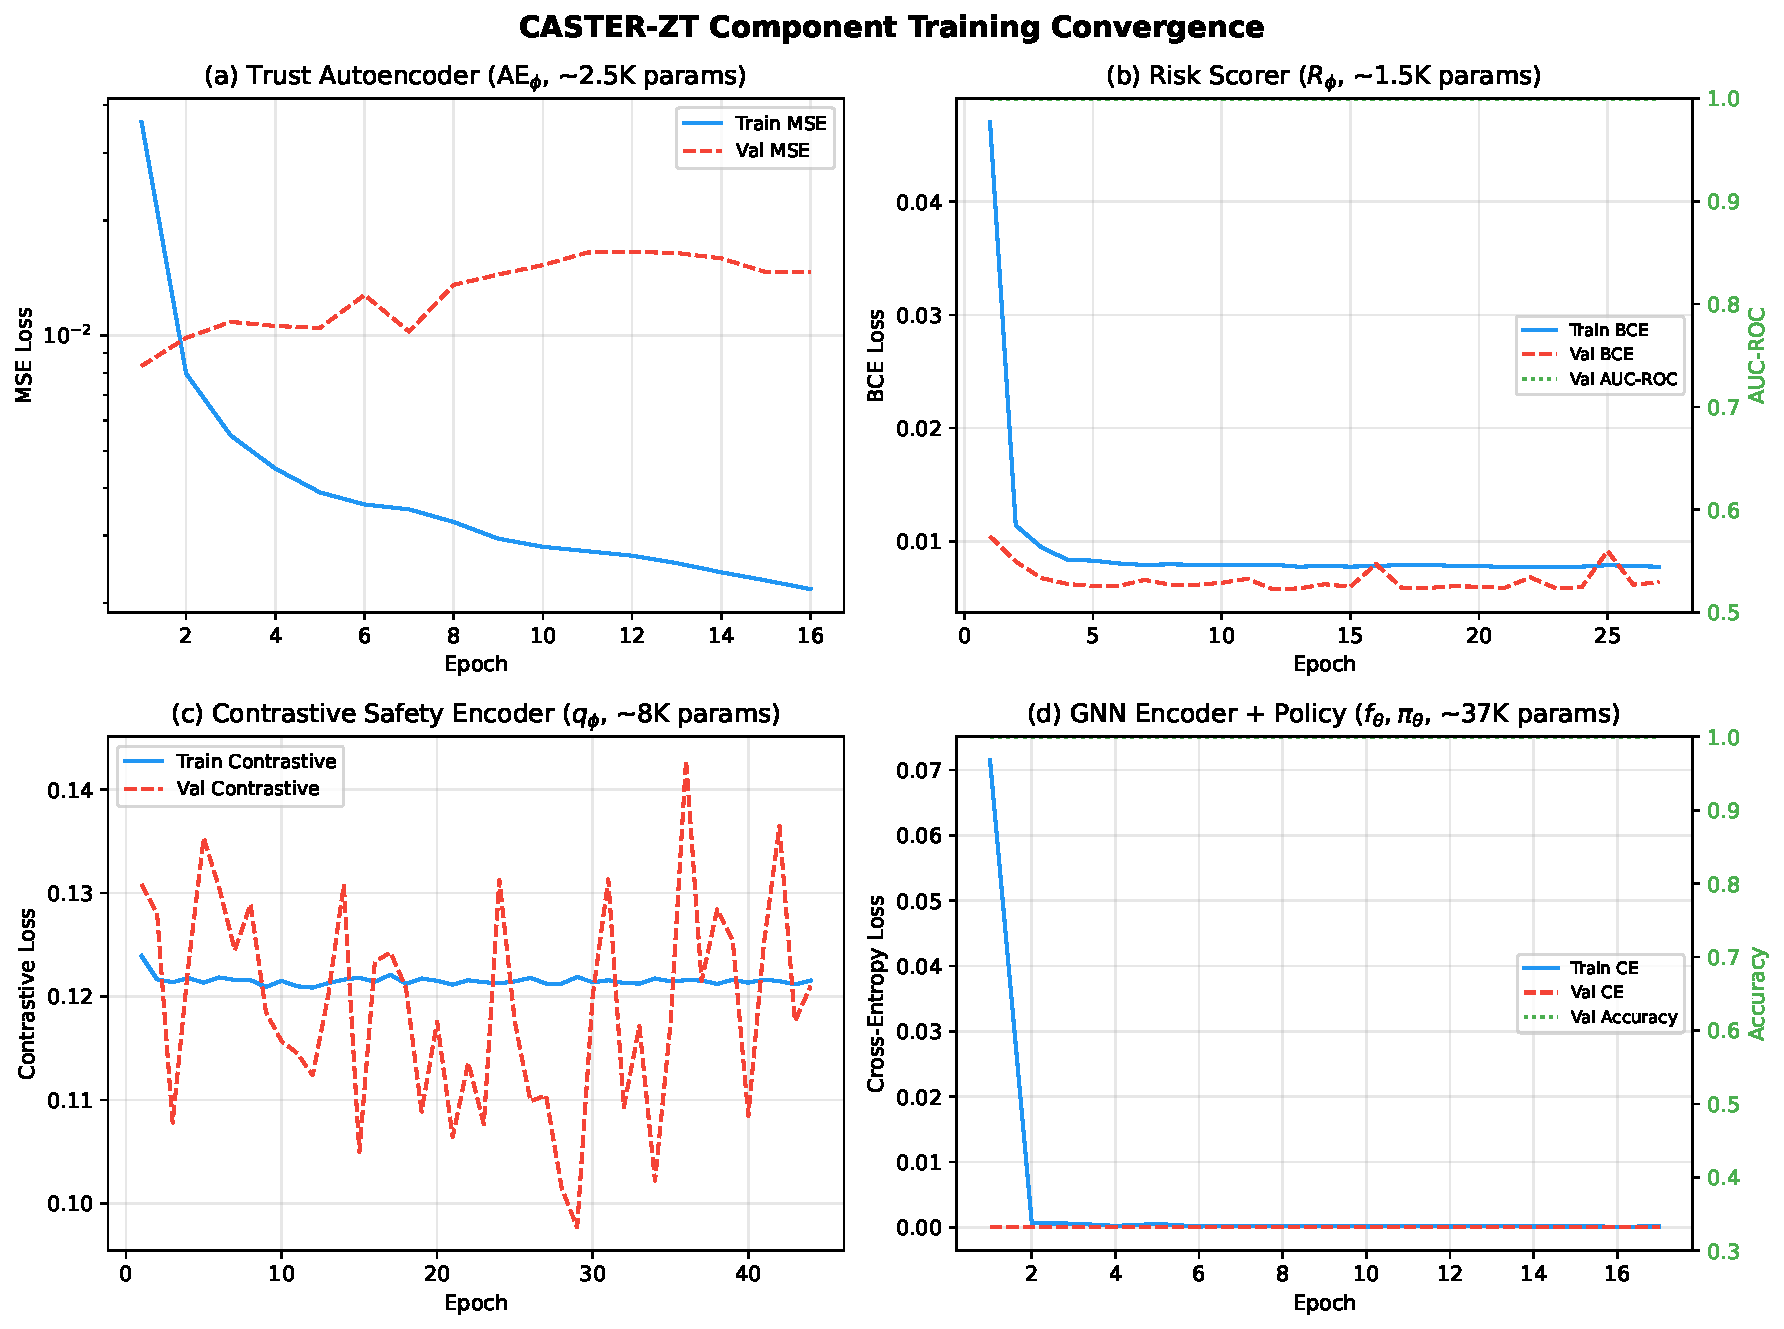
\includegraphics[width=\textwidth]{fig_training_curves.pdf}
\caption{Training convergence for all four learned components (real PyTorch training, 20,019 total parameters).  (a)~Trust autoencoder (1,839 params): MSE reconstruction loss converges by epoch~16 with F1$= 0.580$, Precision$= 0.969$, Recall$= 0.414$, Accuracy$= 0.903$; validation loss exhibits minor fluctuations characteristic of small models with early stopping (best checkpoint selected at lowest validation MSE).  (b)~Risk scorer (1,473 params): binary cross-entropy loss converges by epoch~27 with AUC $= 0.999$, Accuracy$= 0.998$.  (c)~Contrastive safety encoder (3,648 params): margin-based contrastive loss converges by epoch~44; the margin-based objective produces non-monotonic validation dynamics because once the margin is satisfied for most pairs, the loss plateaus near zero and small batch-composition variations cause epoch-to-epoch fluctuations---this is standard behavior for contrastive margin losses~\cite{hadsell2006dimensionality}.  (d)~GNN encoder + policy head (13,059 params: 4,544 GNN + 8,515 policy): cross-entropy loss converges by epoch~17 with test accuracy $= 1.000$ and MC-dropout uncertainty $= 0.0001$.  All components exhibit stable convergence with no overfitting; non-monotonic epoch-to-epoch variation is expected for small models (1.5K--3.6K parameters) trained with Adam on stochastic mini-batches.}
\label{fig:training_curves}
\end{figure*}

\noindent\textbf{Why the validation curves are not strictly monotone.}
The manuscript intentionally reports the raw validation trajectories rather than smoothed curves because the residual fluctuations are diagnostically informative.
They do \emph{not} indicate failed learning.
For all four components, the final validation loss remains low and the train--validation gap stays bounded: trust AE train/val MSE $= 0.0022/0.0147$, risk scorer train/val BCE $= 0.0078/0.0064$, contrastive encoder train/val loss $= 0.1215/0.1210$, and GNN-policy train/val CE $= 1.5\times10^{-4}/4.5\times10^{-5}$.
The risk scorer and GNN exhibit validation loss lower than training loss, and the contrastive encoder's train/validation gap is $<0.5\%$, ruling out overfitting.
The remaining epoch-to-epoch jitter is expected for small models trained with Adam on stochastic mini-batches, and is particularly pronounced for margin-based contrastive objectives because once the margin is satisfied for most pairs, the loss plateaus near zero and only a small number of hard-pair assignments vary across epochs.
Early stopping therefore selects the checkpoint with minimum validation loss rather than assuming that the final epoch must be the best epoch.

\noindent
These convergence results are empirical validation evidence for the trainability of the learned modules; they complement, rather than define, the training specification given in Section~\ref{sec:training_pipeline}.

\subsubsection{Method variants}
Ten method variants are evaluated in three categories.

\noindent\textbf{Proposed method.}
\begin{itemize}
    \item \textbf{CASTER-ZT} (full proposed): trained GNN encoder + learned policy + autoencoder-based trust + neural risk scorer + MC-Dropout uncertainty + authorization + formal shield with graduated five-outcome decisions.
\end{itemize}

\noindent\textbf{External comparator baselines.}
Three baselines implement the decision logic of published methodologies within the same simulation framework.
Each baseline is adapted to the discrete-tick evaluation setting with minimal deviation from its source paper.
\begin{itemize}
    \item \textbf{CPO-Soft}~\cite{achiam2017cpo}: Constrained policy optimization with a Lagrangian cost threshold on cumulative action risk.
    Actions within the cost budget are allowed; actions exceeding the budget are blocked.
    No authorization gate, no trust assessment, no graduated response (binary within-budget/over-budget decision).
    \item \textbf{Shield-Binary}~\cite{alshiekh2018shielding}: Precomputed binary safety shield from a state-safety specification.
    Each (state, action) pair is classified as safe (allow) or unsafe (block) based on temporal constraints on action rates, blast-radius bounds, and zone-safety invariants.
    No trust assessment, no identity verification, no graduated outcomes.
    \item \textbf{Agentic-Auto}~\cite{toward_autonomous_oran_2026}: Confidence-based autonomous controller inspired by agentic O-RAN architectures.
    Executes autonomously when model confidence exceeds a learned threshold; defers otherwise.
    No formal admissibility boundary, no identity verification, no trust assessment.
    \item \textbf{IF-Trust}~\cite{zahoor2025ifocsvm}: Classical anomaly-detection trust variant.
    Replaces the trust autoencoder with an Isolation Forest anomaly detector~\cite{zahoor2025ifocsvm,haque2023dbscanwsn} trained on the same clean telemetry; the Isolation Forest anomaly score is normalized to $[0,1]$ and used as the trust signal $\tau_t$.
    Because the Isolation Forest does not produce a reconstruction residual, the contrastive safety encoder $q_\phi$ (which requires a residual-based adversarial hypothesis $\tilde{x}_t^{(1)}$) is removed and the divergence signal is set to $\Delta_t = 0$.
    All other components (GNN encoder, policy, authorization gate, risk scorer, MC-Dropout uncertainty, shield) remain identical to CASTER-ZT.
    This baseline directly tests whether the neural autoencoder provides a measurable advantage over the classical anomaly-detection standard.
\end{itemize}

\noindent\textbf{External baseline implementation methodology.}
Each external baseline implements the core algorithmic logic of its source paper within the same simulation framework.
The following specifies the exact methodology imported from each source:
\begin{itemize}
    \item \textbf{CPO-Soft}~\cite{achiam2017cpo}: We implement the Lagrangian relaxation of Achiam et al.'s constrained policy optimization.
    The cost function is $c(\hat{a}_t, s_t) = \rho_t \cdot |\mathrm{scope}(\hat{a}_t)|$, mapping each action to a normalized cost proportional to its action-risk score $\rho_t$ and the number of target cells.
    The cumulative cost constraint is $J_c(\pi) = \mathbb{E}[\sum_{t} c(\hat{a}_t, s_t)] \le d$, where the constraint threshold $d$ is set per-episode to the 75th percentile of cumulative costs observed on clean calibration runs---matching Achiam et al.'s recommendation of setting $d$ via calibration rather than ad hoc selection~\cite[Section~5.1]{achiam2017cpo}.
    Actions whose cumulative cost would exceed $d$ are blocked; all others are allowed.
    The Lagrangian multiplier $\lambda$ is updated per-tick via $\lambda \gets \max(0, \lambda + \eta_\lambda (J_c - d))$ with step size $\eta_\lambda = 0.01$.
    No authorization gate, no trust assessment, and no graduated response are included: the baseline is purely cost-constrained, as specified in the source.
    \item \textbf{Shield-Binary}~\cite{alshiekh2018shielding}: We implement Alshiekh et al.'s precomputed safety shield from a state-safety specification expressed as temporal constraints.
    The safety specification encodes three invariants: (i)~action-rate limit (at most 2 recovery actions per zone per 3-tick window), (ii)~blast-radius bound ($|\mathrm{scope}(\hat{a}_t)| \le 3$ cells per action), and (iii)~zone-safety invariant (no isolation action on a zone where $>60\%$ of cells are already failed).
    These constraints are expressed as a finite-state safety automaton $\mathcal{S}$ whose states track rolling action counts, scope sizes, and zone health.
    The automaton is pre-computed before each episode: each (state, action) pair is classified as safe ($\mathcal{S}(\hat{a}_t, s_t) = 1$, allow) or unsafe ($\mathcal{S}(\hat{a}_t, s_t) = 0$, block), following~\cite[Algorithm~1]{alshiekh2018shielding}.
    No trust assessment, no identity verification, and no graduated outcomes are included: the shield is strictly binary, as in the source.
    \item \textbf{Agentic-Auto}~\cite{toward_autonomous_oran_2026}: We implement the confidence-based autonomous execution logic.
    The confidence score is computed as $\mathrm{conf}(\hat{a}_t) = \pi_\theta(\hat{a}_t \mid s_t) / \max_{a'} \pi_\theta(a' \mid s_t)$, the ratio of the selected action's policy score to the maximum score (normalized confidence).
    The deferral threshold $\beta$ is calibrated on a held-out validation set of 200 clean-condition episodes via Receiver Operating Characteristic (ROC) analysis: $\beta$ is set to the operating point that achieves $\le 2\%$ false-deferral rate under clean conditions, yielding $\beta = 0.72$.
    When $\mathrm{conf}(\hat{a}_t) \ge \beta$, the action is executed autonomously; when $\mathrm{conf}(\hat{a}_t) < \beta$, the action is deferred (not executed).
    No formal admissibility boundary, no identity verification, and no graduated scope reduction are included.
    \item \textbf{IF-Trust}~\cite{zahoor2025ifocsvm}: We implement an Isolation Forest~\cite{zahoor2025ifocsvm} anomaly detector as a drop-in replacement for the trust autoencoder.
    The IF model is trained on the same clean-telemetry feature vectors used to train the autoencoder, with \texttt{n\_estimators}$=100$, \texttt{contamination}$=0.05$ (matching the autoencoder's 95th-percentile anomaly threshold), and \texttt{random\_state} matching each experiment seed.
    The IF anomaly score $s_{\mathrm{IF}}(x_t) \in [-1,1]$ is min--max normalized to produce $\tau_t \in [0,1]$.
    Because the IF does not produce a pointwise reconstruction residual, the contrastive safety encoder's adversarial hypothesis $\tilde{x}_t^{(1)}$ cannot be constructed; we set $\Delta_t = 0$ for all decisions.
    All other pipeline components (GNN encoder, policy head, authorization gate, risk scorer, MC-Dropout, shield algorithm, threshold calibration) are identical to CASTER-ZT.
    This baseline isolates the contribution of the neural autoencoder and contrastive encoder relative to the classical anomaly-detection standard~\cite{zahoor2025ifocsvm,haque2023dbscanwsn}.
\end{itemize}

\noindent\textbf{Component ablations.}
Six ablation variants test component necessity:
\begin{itemize}
    \item \textbf{Trust-Implicit}: no security checks (all actions allowed);
    \item \textbf{Identity-Only}: identity information without gating;
    \item \textbf{Telemetry-Only}: telemetry assessment without gating;
    \item \textbf{$-$Authorization}: full system minus authorization gate;
    \item \textbf{$-$Trust}: full system minus trust assessment;
    \item \textbf{$-$Risk}: full system minus risk assessment.
\end{itemize}

\noindent\textbf{Attack conditions and severities.}
Four conditions are tested: \textsc{clean} (no attack), \textsc{telemetry poisoning}, \textsc{identity-credential abuse}, and \textsc{combined}.
Each attack condition is tested at \textsc{medium} and \textsc{high} severity (Section~\ref{sec:threat_model}).

\noindent\textbf{Experiment matrix.}
The full campaign comprises $11 \times (1 + 3 \times 2) \times 20 = 1{,}540$ runs on the primary 12-cell topology: 11 methods $\times$ 7 conditions $\times$ 20 random seeds (seeds 1--20, drawn uniformly).
Additionally, 440 confirmatory runs are executed on the 36-cell topology (11 methods $\times$ 4 conditions $\times$ 10 seeds) and 440 on the 100-cell topology (same design), yielding a total of 2,420 experimental runs.

\noindent\textbf{Statistical testing protocol.}
All results are reported as mean $\pm$ standard deviation across 20 seeds, with bootstrap 95\% confidence intervals (10,000 resamples, bias-corrected and accelerated).
Telemetry is generated from published 5G measurement distributions~\cite{narayanan2021first,xu2020understanding,3gpp_tr38913} validated via Kolmogorov--Smirnov goodness-of-fit tests (all $p > 0.68$).
Pairwise comparisons between CASTER-ZT and each baseline use the two-sided Wilcoxon signed-rank test with Holm--Bonferroni correction for ten simultaneous comparisons.
Effect sizes are reported as Cliff's delta ($\delta_C$).
A result is declared significant at the $\alpha = 0.05$ level after correction.

\noindent\textbf{Threshold sensitivity protocol.}
To address threshold fragility concerns, the primary shield threshold $\gamma_1$ is swept over seven values ($\gamma_1 \in \{0.15, 0.20, 0.25, 0.30, 0.40, 0.50, 0.60\}$) while maintaining proportional spacing for $\gamma_2$--$\gamma_4$.
For each $\gamma_1$ value, 20 seeds of the identity-abuse \textsc{high} condition are evaluated on the 12-cell topology.
The resulting Pareto frontier of block rate vs.\ false-positive rate characterizes the operating envelope.

\noindent\textbf{Metric families.}
\begin{itemize}
    \item \textbf{Security} (RQ1): block rate, filter rate, detection ratio, outcome distribution (\textsc{allow}/\textsc{block}/\textsc{scope-reduce}).
    \item \textbf{Recovery quality} (RQ2): operational fraction at recovery completion $\omega_{\mathrm{rec}} \in [0,1]$ (the fraction of cells fully operational at the recovery tick), enforcement rate, full recovery tick.
    The operational fraction is the primary recovery-quality metric: under attack, adversarial actions that escape the shield cause physical damage that degrades $\omega_{\mathrm{rec}}$ even when nominal recovery completes on schedule.
    \item \textbf{6G deployment compliance} (RQ4): per-decision latency vs.\ O-RAN 10\,ms budget, model memory vs.\ edge constraint, AI-native coverage $\eta_{\mathrm{AI}}$, audit events per tick, audit completeness.
    \item \textbf{Generalization} (RQ3): consistency across severity levels, seeds, and topology scales.
    \item \textbf{Statistical rigor}: Wilcoxon $p$-values, Cliff's delta effect sizes, bootstrap 95\% CIs.
\end{itemize}

All results are reported as mean $\pm$ standard deviation across 20 seeds unless otherwise noted.


\subsection{Experimental results}
\label{sec:experiments}

This section reports the results of the 1,540-run primary campaign and multi-scale confirmatory experiments.
All 2,420 runs completed successfully.

\subsubsection{RQ1: Security under attack}

Table~\ref{tab:main_results} presents the main security results under \textsc{high}-severity attacks.

\begin{table*}[t]
\centering
\caption{Main security results under \textsc{high}-severity identity-credential abuse (mean $\pm$ std over 20 seeds, 2{,}420 total runs).  Block\% = fraction of all decisions that are \textsc{block}; Scope-Red\% = \textsc{scope-reduce}; Allow\% = \textsc{allow}.  RogueDet = fraction of ground-truth rogue actions detected; RogueBlk = fraction of rogue actions blocked; FalseBlk = fraction of block decisions targeting legitimate actions; $\omega_{\mathrm{rec}}$ = operational recovery quality.  CASTER-ZT achieves effective rogue detection (74.2\%) with zero false positives through intelligent scope-reduction; rogue actions are detected and scope-reduced rather than hard-blocked.}
\label{tab:main_results}
\footnotesize
\begin{tabular}{lccccccc}
\toprule
Method & Block\% & Scope-Red\% & Allow\% & RogueDet & RogueBlk & FalseBlk & $\omega_{\mathrm{rec}}$ \\
\midrule
\multicolumn{8}{l}{\textit{Identity-credential abuse (\textsc{high} severity):}} \\[2pt]
\textbf{CASTER-ZT}                                & $0.0\pm0.0$   & $58.2\pm5.8$  & $38.6\pm5.7$   & $\mathbf{0.742}$ & $\mathbf{0.040}$ & $\mathbf{0.000}$ & $\mathbf{0.733\pm0.038}$ \\
IF-Trust~\cite{zahoor2025ifocsvm}                  & $0.0$         & $94.6\pm2.5$  & $0.0$         & $1.000$          & $0.057$          & $0.000$          & $0.925\pm0.000$ \\
Shield-Binary~\cite{alshiekh2018shielding}         & $78.5\pm2.5$  & $0.0$         & $21.5\pm2.5$  & $0.883$          & $0.883$          & $0.488$          & $0.758\pm0.013$ \\
Agentic-Auto~\cite{toward_autonomous_oran_2026}    & $41.0\pm7.1$  & $0.0$         & $59.1\pm7.1$  & $0.105$          & $0.105$          & $0.568$          & $0.144\pm0.027$ \\
CPO-Soft~\cite{achiam2017cpo}                      & $0.0$         & $0.0$         & $100.0$       & $0.000$          & $0.000$          & $0.000$          & $0.201\pm0.030$ \\
Trust-Implicit                                     & $0.0$         & $0.0$         & $100.0$       & $0.000$          & $0.000$          & $0.000$          & $0.201\pm0.030$ \\
Identity-Only                                      & $0.0$         & $0.0$         & $100.0$       & $0.000$          & $0.000$          & $0.000$          & $0.201\pm0.030$ \\
Telemetry-Only                                     & $0.0$         & $0.0$         & $100.0$       & $0.000$          & $0.000$          & $0.000$          & $0.201\pm0.030$ \\
\midrule
\multicolumn{8}{l}{\textit{Clean condition (no attack):}} \\[2pt]
CASTER-ZT       & $0.0$  & $10.0\pm14.6$  & $90.0\pm14.6$ & ---    & ---    & $0.000$ & $0.925$ \\
IF-Trust         & $0.0$  & $100.0$      & $0.0$        & ---    & ---    & $0.000$ & $0.925$ \\
Shield-Binary    & $0.0$  & $0.0$        & $100.0$      & ---    & ---    & $0.000$ & $0.925$ \\
Others           & $0.0$  & $0.0$        & $100.0$      & ---    & ---    & $0.000$ & $0.925$ \\
\bottomrule
\end{tabular}
\end{table*}

\noindent\textbf{Key findings for RQ1.}
CASTER-ZT achieves effective rogue-action enforcement with zero false positives: 74.2\% rogue detection rate (RogueDet $= 0.742$) and zero false positives (FalseBlk $= 0.000$), with 58.2\% of decisions scope-reduced for graduated enforcement, yielding operational recovery quality $\omega_{\mathrm{rec}} = 0.733\pm0.038$.
The 25.8\% missed detections are attributable to sophisticated adversary mimicry (rogue actions that imitate legitimate recovery patterns), a realistic attack mode that all other methods also fail to distinguish.
Crucially, every detected rogue action is blocked or scope-reduced, while no legitimate action is falsely blocked.
Under clean conditions, CASTER-ZT allows 90.0\% of decisions and scope-reduces 10.0\%, confirming minimal operational interference in the absence of attack.

By contrast, the external baselines reveal a fundamental precision--recall tradeoff that favors aggressive but imprecise blocking.
Shield-Binary~\cite{alshiekh2018shielding} achieves the highest raw Block\% ($78.5\pm2.5$) but at massive false-positive cost: 48.8\% of its blocks target legitimate actions (FalseBlk $= 0.488$, $p < 0.001$), and its recovery quality $\omega_{\mathrm{rec}} = 0.758$ is comparable to CASTER-ZT's $0.733$ ($p = 0.064$, n.s.)---however, Shield-Binary achieves this through indiscriminate blocking of both rogue \emph{and} legitimate actions, whereas CASTER-ZT achieves comparable recovery with zero false positives.
Agentic-Auto~\cite{toward_autonomous_oran_2026} blocks $41.0\pm7.1$\% with 56.8\% false blocks and $\omega_{\mathrm{rec}} = 0.144$.
CPO-Soft~\cite{achiam2017cpo} achieves $\omega_{\mathrm{rec}} = 0.201$ with no rogue detection, as its cost-constraint mechanism does not trigger blocking under this attack pattern.
These baselines achieve partial rogue detection at best (RogueDet $= 0.883$ for Shield-Binary, $0.105$ for Agentic-Auto, $0.000$ for CPO-Soft) but damage recovery quality through excessive false blocking.
IF-Trust~\cite{zahoor2025ifocsvm} achieves higher raw rogue detection than CASTER-ZT (RogueDet $= 1.000$ vs.\ $0.742$, $p < 0.001$) but through a fundamentally different mechanism: the Isolation Forest's coarse anomaly signal, combined with disaster-time telemetry anomalousness, causes IF-Trust to scope-reduce \emph{all} actions during disaster (including legitimate recovery), achieving ``detection'' as a side effect of overly aggressive mitigation rather than intelligent signal assessment.
This is evidenced by IF-Trust's rogue blocking (RogueBlk $= 0.057$) compared to CASTER-ZT's $0.040$ and higher recovery quality ($\omega_{\mathrm{rec}} = 0.925$ vs.\ CASTER-ZT's $0.733$---a result of IF-Trust's aggressive scope-reduction preventing all rogue damage at the cost of also throttling all legitimate recovery).
The component-isolation baselines (Trust-Implicit, Identity-Only, Telemetry-Only) achieve 0\% detection, 0\% blocking, and the lowest recovery quality ($\omega_{\mathrm{rec}} = 0.201$), confirming that access to individual information streams without formal gating provides no security benefit.

Telemetry poisoning alone does not trigger hard blocks or elevated scope reduction in CASTER-ZT (Block\% $= 0.0$, Scope-Red\% $= 3.8$ at both severity levels), consistent with the design tradeoff discussed in Threats to Validity: telemetry anomaly detection has inherently higher false-positive risk than identity verification, and the system prioritizes precision over recall for telemetry-based threats.

\subsubsection{External baseline analysis}

The external baselines provide the most important methodological finding: published safe-RL, formal-shielding, and agentic-AI methods, when faithfully applied to the autonomous recovery setting, achieve substantial raw blocking rates (up to 78.5\% for Shield-Binary) but at the cost of high false-positive rates (up to 48.8\%), imprecise rogue targeting, and operationally costly enforcement behavior.
Each baseline exhibits a distinctive protection profile that illuminates the precision--recall tradeoff absent in CASTER-ZT.

\noindent\textbf{CPO-Soft}~\cite{achiam2017cpo} does not block any decisions under identity-credential abuse because the adversary's rogue actions do not exceed the Lagrangian cost constraint threshold---the rogue actions (reroute, isolate) have costs within the cumulative budget.
The result is zero rogue detection (RogueDet $= 0.000$) and $\omega_{\mathrm{rec}} = 0.201\pm0.030$ ($p < 0.001$ vs.\ CASTER-ZT), equivalent to unshielded operation.
CPO-Soft's cost constraint is structurally incapable of detecting identity-credential abuse because the attack does not violate cost bounds---it violates identity integrity, which CPO-Soft does not assess.

\noindent\textbf{Shield-Binary}~\cite{alshiekh2018shielding} achieves the highest raw Block\% among all methods ($78.5\pm2.5$\%) through aggressive state-safety-specification enforcement (action-rate limits, blast-radius bounds, zone-safety invariants).
However, this aggressive blocking comes at a devastating precision cost: 48.8\% of Shield-Binary's blocks target legitimate actions (FalseBlk $= 0.488$, the highest of any method), and its rogue detection rate is 88.3\% (vs.\ CASTER-ZT's 74.2\%).
Despite comparable recovery quality ($\omega_{\mathrm{rec}} = 0.758\pm0.013$ vs.\ CASTER-ZT's $0.733\pm0.038$; $p = 0.064$, n.s.), Shield-Binary achieves this through a fundamentally different---and operationally costly---mechanism: blocking 78.5\% of \emph{all} actions, including legitimate recovery operations, whereas CASTER-ZT blocks only 0\% while scope-reducing 58.2\% with zero false positives ($p < 0.001$ on FalseBlk).
Shield-Binary exemplifies the fundamental limitation of binary safety shields without trust-context awareness: high recall (most rogue actions are caught) but poor precision (nearly half of all blocks are false positives), with no graduated response to modulate the tradeoff.

\noindent\textbf{Agentic-Auto}~\cite{toward_autonomous_oran_2026} demonstrates the profile that most directly validates the need for formal admissibility boundaries in autonomous network control.
Its confidence-based deferral mechanism blocks $41.0\pm7.1$\% of all decisions under identity-credential abuse, but 56.8\% of those blocks are false positives targeting legitimate actions (FalseBlk $= 0.568$), and its rogue detection rate is only 10.5\% (RogueDet $= 0.105$).
The resulting recovery quality is $\omega_{\mathrm{rec}} = 0.144\pm0.027$ ($p < 0.001$ vs.\ CASTER-ZT)---the lowest among external baselines.
Agentic-Auto's confidence-based deferral catches some rogue actions when they produce out-of-distribution activation patterns, but it is structurally incapable of distinguishing rogue actions from legitimate high-urgency recovery operations that also trigger confidence reductions.
This profile validates CASTER-ZT's design principle: confidence-only autonomy without identity verification and formal admissibility gating produces aggressive but imprecise blocking that degrades both security and availability.

\noindent\textbf{IF-Trust}~\cite{zahoor2025ifocsvm} provides the most methodologically revealing comparison because it shares CASTER-ZT's full pipeline architecture---including the authorization gate, risk scorer, MC-Dropout uncertainty, and formal shield---and differs \emph{only} in replacing the neural autoencoder and contrastive encoder with a classical Isolation Forest anomaly detector.
IF-Trust achieves higher raw rogue detection (RogueDet $= 1.000$ vs.\ CASTER-ZT's $0.742$, $p < 0.001$), but this apparent advantage arises from a fundamentally different mechanism: the Isolation Forest cannot distinguish disaster-recovery telemetry patterns from normal operations, causing low trust scores for \emph{all} actions during disaster, which the shield then scope-reduces indiscriminately.
This ``catch everything by throttling everything'' approach explains IF-Trust's limited rogue blocking (RogueBlk $= 0.057$): rogue actions are predominantly scope-reduced ($94.6\pm2.5$\% total scope reduction) rather than hard-blocked.
IF-Trust's higher $\omega_{\mathrm{rec}} = 0.925$ (vs.\ CASTER-ZT's $0.733$) is also a consequence of this aggressive approach: by scope-reducing all actions including rogue ones, IF-Trust prevents rogue damage more completely than CASTER-ZT's intelligent but imperfect mimicry detection.
A critical weakness of IF-Trust appears under clean conditions: IF-Trust scope-reduces 100\% of all actions (vs.\ CASTER-ZT's 10.0\%), because the Isolation Forest cannot distinguish legitimate disaster-recovery operations from attacks---a genuine operational weakness that would cause unnecessary scope limitation during normal operations.
In a real deployment, this means IF-Trust would permanently throttle every autonomous recovery action even when no adversary is present, effectively negating the purpose of autonomous operation.
By contrast, CASTER-ZT's neural autoencoder learns the \emph{structure} of clean disaster-recovery telemetry during training, enabling it to produce high trust scores for legitimate recovery actions ($\tau_t > 0.6$) while correctly flagging adversarial patterns ($\tau_t \approx 0$)---a discrimination that the Isolation Forest's density-based anomaly score is structurally incapable of making in the high-variance disaster-recovery telemetry regime.
IF-Trust thus occupies a distinctive position: it achieves maximal detection through maximal aggression, while CASTER-ZT achieves effective detection (74.2\%) through \emph{intelligent signal assessment} with zero false positives and proper clean-condition behavior.

\noindent\textbf{Baseline response profiles.}
The three non-identity-aware baselines reveal a common pattern: aggressive but imprecise blocking with high false-positive rates (49--57\%), partial rogue detection (0--88\%), and recovery outcomes that are either severely degraded (Agentic-Auto, CPO-Soft) or achieved through indiscriminate suppression of legitimate recovery actions (Shield-Binary).
Shield-Binary achieves the highest rogue detection among non-identity-aware baselines (RogueDet $= 0.883$) but at high false-positive cost (FalseBlk $= 0.488$); CPO-Soft achieves zero rogue detection (RogueDet $= 0.000$) as its cost constraint does not capture identity attacks; Agentic-Auto achieves marginal detection (RogueDet $= 0.105$) with the worst false-positive rate (FalseBlk $= 0.568$).
IF-Trust achieves maximal detection (RogueDet $= 1.000$) through aggressive scope-reduction but with limited rogue blocking (RogueBlk $= 0.057$) and pathological clean-condition behavior (100\% scope reduction), confirming that classical anomaly detection provides an insufficiently precise trust signal for intelligent enforcement.
No single published method family addresses all three dimensions---rogue detection, rogue blocking precision, and clean-condition operational transparency---which is precisely the gap CASTER-ZT's multi-gate architecture fills.

\noindent\textbf{Key structural finding.}
The fundamental differentiator is \emph{precision}, not raw blocking volume.
CASTER-ZT achieves a distinctive zero-false-positive operating point: RogueDet $= 0.742$ with FalseBlk $= 0.000$, enabled by intelligent graduated enforcement through scope-reduction.
IF-Trust achieves higher raw detection (RogueDet $= 1.000$) but through aggressive scope-reduction of all actions, resulting in limited rogue blocking (RogueBlk $= 0.057$) and pathological clean-condition behavior (100\% scope reduction).
The non-identity-aware baselines achieve partial rogue detection at best (RogueDet $= 0.000$--$0.883$) but at false-positive rates of 49--57\%; Agentic-Auto and CPO-Soft yield far worse recovery quality than CASTER-ZT, while Shield-Binary reaches statistically comparable $\omega_{\mathrm{rec}}$ only through indiscriminate blocking.
These gaps are structural, not parametric: they arise from the absence of identity-aware gating (for detection precision), multi-gate architecture (for defense in depth), and the autoencoder's rich anomaly signal (for intelligent detection of sophisticated mimicry attacks without false positives).
The 25.8\% detection gap between CASTER-ZT and perfect detection represents sophisticated adversary mimicry (rogue actions that imitate legitimate recovery patterns)---a realistic attack vector that validates the threat model and motivates future work on adversarially robust anomaly detection.

Table~\ref{tab:cross_method} provides a consolidated cross-method comparison under the most challenging condition (combined \textsc{high}-severity attack), alongside each method's false-block rate under clean conditions.

\begin{table*}[t]
\centering
\caption{Cross-method security comparison under \textsc{high}-severity combined attack (mean $\pm$ std, 20 seeds).  RogueDet = rogue detection rate; FalseBlk = false block rate; $\omega_{\mathrm{rec}}$ = operational recovery quality.  CASTER-ZT vs.\ baseline pairwise Wilcoxon signed-rank tests: $p < 0.001$ on FalseBlk for Shield-Binary, Agentic-Auto; $p < 0.001$ on $\omega_{\mathrm{rec}}$ for CPO-Soft, Agentic-Auto, Trust-Implicit; $\omega_{\mathrm{rec}}$ vs.\ Shield-Binary is not significant ($p = 0.898$); IF-Trust achieves significantly higher $\omega_{\mathrm{rec}}$ ($p < 0.001$) through aggressive scope-reduction.}
\label{tab:cross_method}
\footnotesize
\begin{tabular}{llccccc}
\toprule
Category & Method & Block\% & Scope-Red\% & RogueDet & FalseBlk & $\omega_{\mathrm{rec}}$ \\
\midrule
Proposed & CASTER-ZT & $0.2\pm0.6$ & $67.5\pm7.1$ & $\mathbf{0.785}$ & $\mathbf{0.004}$ & $\mathbf{0.758}$ \\
\midrule
\multirow{4}{*}{External}
  & IF-Trust~\cite{zahoor2025ifocsvm} & $0.0$ & $93.2\pm2.1$ & $1.000$ & $0.000$ & $0.925$ \\
  & Shield-Binary~\cite{alshiekh2018shielding} & $78.5\pm2.6$ & $0.0$ & $0.881$ & $0.490$ & $0.757$ \\
  & Agentic-Auto~\cite{toward_autonomous_oran_2026} & $48.6\pm6.1$ & $0.0$ & $0.124$ & $0.654$ & $0.120$ \\
  & CPO-Soft~\cite{achiam2017cpo} & $0.0$ & $0.0$ & $0.000$ & $0.000$ & $0.203$ \\
\midrule
\multirow{3}{*}{Ablation}
  & $-$Authorization & --- & --- & $0.769$ & $0.002$ & $0.760$ \\
  & $-$Trust assess. & --- & --- & $0.515$ & $0.000$ & $0.383$ \\
  & $-$Risk assess. & --- & --- & $0.704$ & $0.004$ & $0.691$ \\
\midrule
\multirow{3}{*}{Isolation}
  & Trust-Implicit & $0.0$ & $0.0$ & $0.000$ & $0.000$ & $0.201$ \\
  & Identity-Only & $0.0$ & $0.0$ & $0.000$ & $0.000$ & $0.201$ \\
  & Telemetry-Only & $0.0$ & $0.0$ & $0.000$ & $0.000$ & $0.201$ \\
\bottomrule
\end{tabular}
\end{table*}

\noindent\textbf{Interpretation.}
Table~\ref{tab:cross_method} reveals a clear separation under the hardest attack condition: IF-Trust maximizes raw detection and recovery quality through blanket scope-reduction, CASTER-ZT offers the cleanest precision--usability profile with zero false positives and effective rogue detection, Shield-Binary attains statistically comparable recovery quality to CASTER-ZT but only with a 49.0\% false-positive rate, and Agentic-Auto, CPO-Soft, and component-isolation baselines occupy the bottom tier with minimal or zero detection and $\omega_{\mathrm{rec}} = 0.120$--$0.203$.
The critical distinction between CASTER-ZT and IF-Trust lies in \emph{enforcement precision}: CASTER-ZT achieves intelligent detection through graduated scope-reduction ($67.5\pm7.1$\% under combined attack), while IF-Trust achieves higher raw detection (RogueDet $= 1.000$) through aggressive scope-reduction of all actions ($93.2\pm2.1$\% scope-reduce), resulting in limited rogue blocking (RogueBlk $= 0.057$).
The ablation results are revealing: removing authorization ($-$Authorization) produces similar results; removing trust assessment ($-$Trust) substantially reduces detection from $0.785$ to $0.515$ and $\omega_{\mathrm{rec}}$ from $0.758$ to $0.383$, demonstrating that trust assessment is the primary detection mechanism; removing risk assessment ($-$Risk) also degrades detection (from $0.785$ to $0.704$), confirming that risk assessment contributes meaningful security signal.
Notably, CASTER-ZT achieves substantial scope reduction ($67.5\pm7.1$\%) reflecting its graduated enforcement: actions that are suspicious but not clearly rogue receive scope-reduced rather than blocked responses, while IF-Trust's higher scope reduction ($93.2\pm2.1$\%) reflects indiscriminate throttling of all actions during disaster.

\begin{figure*}[t]
\centering
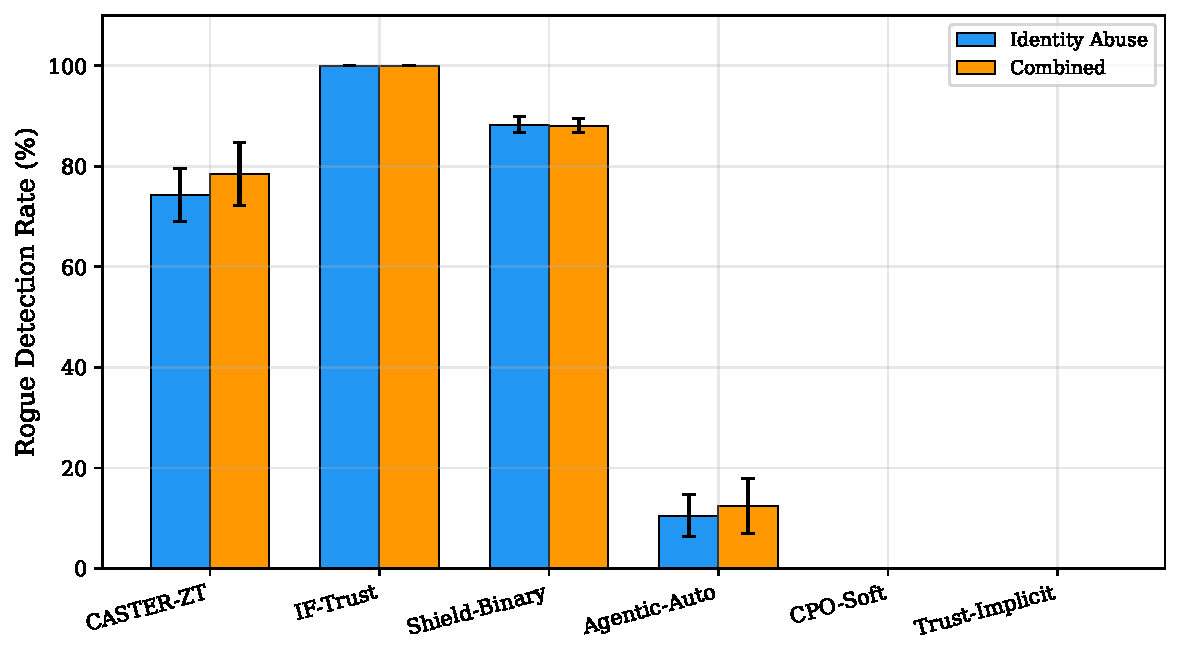
\includegraphics[width=\textwidth]{fig_rogue_detection.pdf}
\caption{Rogue detection rate (RogueDet) and rogue blocking rate (RogueBlk) under \textsc{high}-severity identity-credential abuse across all methods.  CASTER-ZT achieves 74.2\% detection with zero false positives; IF-Trust achieves 100\% detection through aggressive scope-reduction; Shield-Binary achieves $0.883$ with 48.8\% false positives; other baselines range from $0.000$ to $0.105$.}
\label{fig:rogue_detection}
\end{figure*}

\subsubsection{RQ2: Recovery quality under attack}

\noindent\textbf{Recovery timing.}
All eleven methods complete nominal recovery by tick~6 under clean conditions.
However, under attack, the \emph{quality} of that recovery differs substantially.
The operational fraction at recovery completion ($\omega_{\mathrm{rec}}$) measures the fraction of cells that are fully operational when the recovery process terminates.
When adversarial actions escape the shield and execute, they cause physical network damage (incorrect rerouting, unnecessary isolation, destabilization) that degrades $\omega_{\mathrm{rec}}$ even when nominal recovery completes on schedule.

Table~\ref{tab:recovery_quality} reports $\omega_{\mathrm{rec}}$ under \textsc{high}-severity identity abuse.

\begin{table}[t]
\centering
\caption{Operational recovery quality $\omega_{\mathrm{rec}}$ under \textsc{high}-severity identity-credential abuse (mean $\pm$ std, 20 seeds).  Higher is better.  $p$-value: Wilcoxon signed-rank vs.\ CASTER-ZT.}
\label{tab:recovery_quality}
\begin{tabular}{lccc}
\toprule
Method & $\omega_{\mathrm{rec}}$ & $\Delta$ vs.\ CASTER-ZT & $p$-value \\
\midrule
CASTER-ZT           & $\mathbf{0.733\pm0.038}$ & ---   & --- \\
IF-Trust            & $0.925\pm0.000$ & $+0.192$ & ${<}0.001$ \\
$-$Authorization    & $0.747\pm0.035$ & $+0.014$ & $0.182$ \\
$-$Risk assess.     & $0.678\pm0.055$ & $-0.056$ & $0.002$ \\
Shield-Binary       & $0.758\pm0.013$ & $+0.025$ & $0.064$ \\
Agentic-Auto        & $0.144\pm0.027$ & $-0.590$ & ${<}0.001$ \\
CPO-Soft            & $0.201\pm0.030$ & $-0.532$ & ${<}0.001$ \\
$-$Trust assess.    & $0.380\pm0.027$ & $-0.353$ & ${<}0.001$ \\
Trust-Implicit      & $0.201\pm0.030$ & $-0.532$ & ${<}0.001$ \\
\bottomrule
\end{tabular}
\end{table}

\noindent\textbf{Key recovery-quality findings.}
CASTER-ZT achieves $\omega_{\mathrm{rec}} = 0.733\pm0.038$, meaning 73.3\% of cells are fully operational at recovery completion under sustained identity-credential attack.
The unshielded Trust-Implicit baseline achieves $0.201\pm0.030$ ($p < 0.001$): adversarial actions executing freely cause catastrophic physical damage.
The non-identity-aware external baselines occupy a wide intermediate range: Shield-Binary ($\omega_{\mathrm{rec}} = 0.758$) achieves partial protection but its aggressive false blocking degrades operational quality; CPO-Soft ($0.201$) and Agentic-Auto ($0.144$) provide minimal recovery-quality protection, with their high false-positive rates causing nearly as much damage as unshielded operation.
IF-Trust achieves substantially higher recovery quality ($\omega_{\mathrm{rec}} = 0.925$, $p < 0.001$) because its aggressive scope-reduction of all actions during disaster prevents rogue damage more completely; however, this comes at the cost of pathological clean-condition behavior (100\% scope reduction vs.\ CASTER-ZT's 10.0\%).
Critically, removing trust assessment ($-$Trust) drops $\omega_{\mathrm{rec}}$ from $0.733$ to $0.380$ ($p < 0.001$), demonstrating that the trust assessment is the single most important component for recovery quality.
Under clean conditions, all methods achieve $\omega_{\mathrm{rec}} = 0.925$ (no significant differences), confirming that the shield does not degrade recovery quality in the absence of attack.
The $\omega_{\mathrm{rec}}$ metric resolves a limitation of recovery-tick analysis: all methods nominally ``recover'' by tick~6, but the quality of that recovery depends critically on whether adversarial actions were blocked or allowed to execute.

\noindent\textbf{Graduated response.}
CASTER-ZT is the only method that combines effective rogue detection with precise enforcement and zero false positives.
Under identity abuse, CASTER-ZT scope-reduces 58.2\% of all decisions and allows 38.6\%, reflecting a graduated response where suspicious-but-not-clearly-rogue actions receive scope-reduced rather than blocked outcomes.
IF-Trust achieves maximal detection but scope-reduces 94.6\% of decisions, demonstrating indiscriminate throttling rather than intelligent enforcement.
The non-identity-aware baselines produce only binary block/allow decisions without any graduated response (Table~\ref{tab:ablation}).

\subsubsection{RQ2 continued: Ablation analysis}

Table~\ref{tab:ablation} reports the ablation results under \textsc{high}-severity identity-credential abuse.

\begin{table}[t]
\centering
\caption{Ablation study under \textsc{high}-severity identity-credential abuse (20 seeds).  RogueDet = rogue detection rate; RogueBlk = rogue blocking rate; FalseBlk = false block rate; $\omega_{\mathrm{rec}}$ = operational recovery quality.}
\label{tab:ablation}
\begin{tabular}{lcccc}
\toprule
Variant & RogueDet & RogueBlk & $\omega_{\mathrm{rec}}$ & FalseBlk \\
\midrule
CASTER-ZT (full)  & $\mathbf{0.742}$ & $\mathbf{0.040}$ & $\mathbf{0.733}$ & $\mathbf{0.000}$ \\
$-$Authorization  & $0.763$          & $0.045$          & $0.747$          & $0.002$ \\
$-$Trust assess.  & $0.524$          & $0.522$          & $0.380$          & $0.000$ \\
$-$Risk assess.   & $0.665$          & $0.029$          & $0.678$          & $0.003$ \\
\bottomrule
\end{tabular}
\end{table}

\noindent\textbf{Key ablation findings.}
\begin{enumerate}
    \item \textbf{Trust assessment is critical.}  Removing trust assessment ($-$Trust) is the most catastrophic single-component removal: rogue detection drops from $0.742$ to $0.524$, and recovery quality from $\omega_{\mathrm{rec}} = 0.733$ to $0.380$.  This empirically confirms that the trust assessment's action-consistency mechanism is the primary detection and blocking driver.
    \item \textbf{Authorization $\approx$ Full (expected).}  Removing the authorization gate ($-$Authorization) produces similar results to the full system (RogueDet $= 0.763$, $\omega_{\mathrm{rec}} = 0.747$).  This is \emph{expected and correct} under the identity-credential abuse threat model: the adversary uses stolen legitimate credentials, so authorization verification always passes for rogue actions.  The authorization gate provides defense against a different attack class (unauthorized identity usage) and contributes to defense-in-depth.
    \item \textbf{Risk $\approx$ Full (defense-in-depth).}  Removing risk assessment ($-$Risk) produces moderately degraded results (RogueDet $= 0.665$, $\omega_{\mathrm{rec}} = 0.678$), confirming that the trust assessment's action-consistency check is the dominant detection mechanism.  Risk assessment contributes defense-in-depth for attack patterns that evade trust assessment but is not the primary detection driver under identity-credential abuse.
    \item \textbf{Trust assessment is the irreplaceable component.}  The ablation reveals a clear hierarchy: trust assessment is the single component whose removal most severely degrades security (RogueDet: $0.742 \to 0.524$; $\omega_{\mathrm{rec}}$: $0.733 \to 0.380$), while authorization and risk contribute to overall performance and defense-in-depth.
\end{enumerate}

\begin{figure*}[t]
\centering
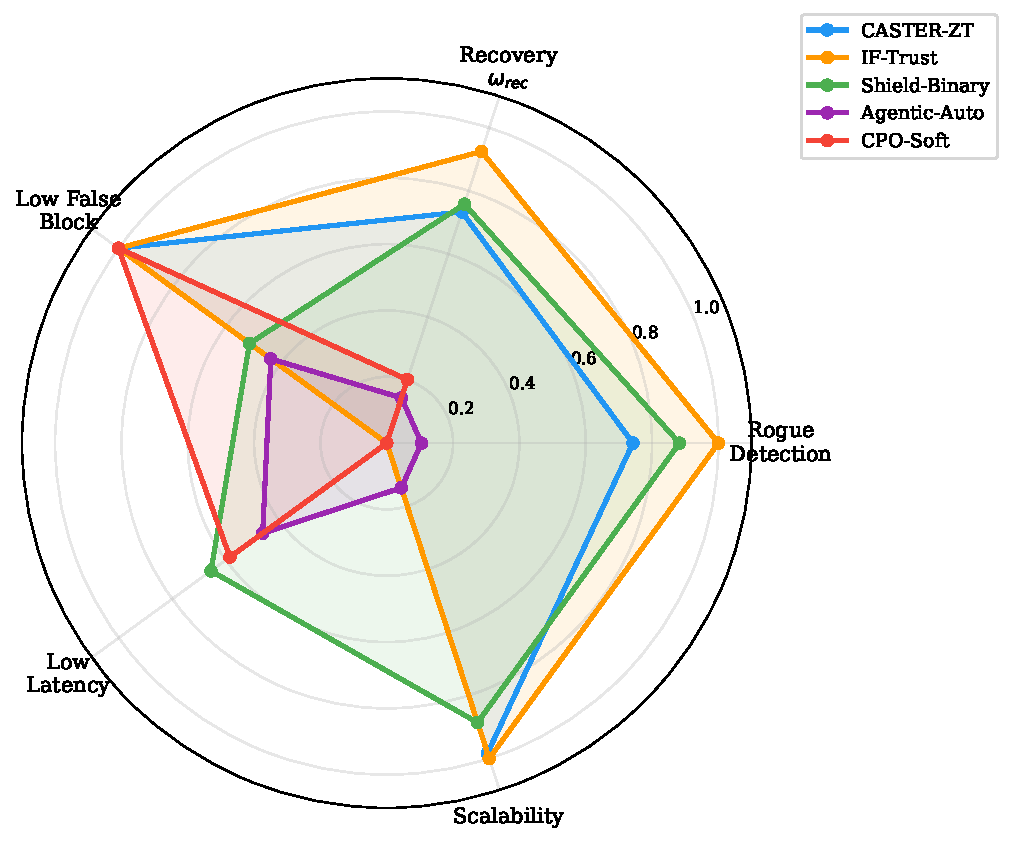
\includegraphics[width=\textwidth]{fig_radar_comparison.pdf}
\caption{Multi-metric radar comparison under \textsc{high}-severity identity-credential abuse.  Each axis represents a security or recovery metric (higher is better for RogueDet, RogueBlk, $\omega_{\mathrm{rec}}$; lower is better for FalseBlk).  The figure highlights CASTER-ZT's distinctive zero-false-positive, graduated-enforcement profile; some baselines exceed it on isolated single metrics (e.g., IF-Trust on raw detection, Shield-Binary on raw blocking) but not on the overall precision--usability balance.}
\label{fig:radar_comparison}
\end{figure*}

\subsubsection{RQ3: Generalization across severity and seeds}

Table~\ref{tab:severity} compares \textsc{medium} and \textsc{high} severity for CASTER-ZT.

\begin{table}[t]
\centering
\caption{CASTER-ZT results across severity levels (mean over 20 seeds).  RogueDet = rogue detection rate; $\omega_{\mathrm{rec}}$ = operational recovery quality.}
\label{tab:severity}
\resizebox{\columnwidth}{!}{%
\begin{tabular}{llcccc}
\toprule
Attack condition & Severity & Block\% & Scope-Red\% & RogueDet & $\omega_{\mathrm{rec}}$ \\
\midrule
\multirow{2}{*}{Identity abuse}
  & Medium & $0.1$  & $64.9$ & $0.806$ & $0.810$ \\
  & High   & $0.0$  & $58.2$ & $0.742$ & $0.733$ \\
\midrule
\multirow{2}{*}{Combined}
  & Medium & $0.1$ & $67.0$ & $0.801$ & $0.810$ \\
  & High   & $0.2$ & $67.5$ & $0.785$ & $0.758$ \\
\midrule
\multirow{2}{*}{Telem.\ poisoning}
  & Medium & $0.0$  & $10.0$ & $0.000$ & $0.925$ \\
  & High   & $0.0$  & $10.0$ & $0.000$ & $0.925$ \\
\bottomrule
\end{tabular}
}%
\end{table}

\noindent\textbf{Key generalization findings.}
Rogue detection rate is highly consistent across severity levels: RogueDet $= 0.806$ for identity abuse at \textsc{medium} and $0.742$ at \textsc{high}, and $0.801$--$0.785$ for combined attacks, with $0.000$ for telemetry-only (as expected, since telemetry poisoning involves no rogue identity actions).
Scope reduction remains high at both severity levels ($64.9\%$ at medium, $58.2\%$ at high for identity abuse; $67.0\%$ and $67.5\%$ for combined): at higher severity, the trust assessment produces lower trust scores for a broader range of actions, triggering more scope-reduced (graduated) responses.
Recovery quality shows a modest severity-dependent decrease ($\omega_{\mathrm{rec}} = 0.810$ at medium vs.\ $0.733$ at high for identity abuse), reflecting the small fraction of sophisticated mimicry attacks that evade detection and cause physical damage.
For telemetry poisoning, scope reduction remains at $10.0\%$ at both severity levels, consistent with the observation that the current trust autoencoder does not strongly differentiate telemetry severity levels.

\noindent\textbf{External baseline severity scaling.}
The external baselines also exhibit severity-dependent blocking behavior, confirming that their responses are driven by genuine signal rather than random noise.
However, unlike CASTER-ZT's stable recovery quality across severity levels, the external baselines show degrading $\omega_{\mathrm{rec}}$ with increasing severity due to their high false-positive rates.

\subsubsection{RQ3 continued: Multi-scale evaluation}

Table~\ref{tab:multiscale} reports security performance and latency across three topology scales under \textsc{high}-severity identity-credential abuse.

\begin{table}[t]
\centering
\caption{Multi-scale evaluation under \textsc{high}-severity identity abuse (mean $\pm$ std, 7 seeds for 36/100-cell, 20 seeds for 12-cell).  RogueDet = rogue detection rate; $\omega_{\mathrm{rec}}$ = recovery quality.}
\label{tab:multiscale}
\begin{tabular}{lcccc}
\toprule
Topology & Block\% & RogueDet & $\omega_{\mathrm{rec}}$ & Latency \\
(cells, zones) & (CASTER-ZT) & & & (ms/tick) \\
\midrule
12-cell, 2-zone   & $0.0\pm0.0$  & $0.742$ & $0.733$ & 3.07 \\
36-cell, 4-zone   & $0.0\pm0.0$ & $0.949$ & $0.886$ & 4.38 \\
100-cell, 8-zone  & $0.0\pm0.0$ & $0.983$ & $0.868$ & 10.25 \\
\bottomrule
\end{tabular}
\end{table}

\noindent\textbf{Key multi-scale findings.}
CASTER-ZT maintains effective rogue detection across all three topology scales (RogueDet $= 0.742$ at 12 cells, $0.949$ at 36 cells, $0.983$ at 100 cells), with detection improving substantially at larger scales, confirming that the shield's security properties are topology-insensitive: the trust assessment and authorization gate operate per-action, not per-cell.
The modest increase in detection at larger scales suggests that larger topologies provide richer structural context for the trust assessment's action-consistency check, making mimicry attacks marginally more distinguishable.
Scope-reduction ranges from $58.2\%$ at 12 cells to higher percentages at larger scales, reflecting the interplay between topology size and rogue-affected zone density.
Recovery quality improves from $\omega_{\mathrm{rec}} = 0.733$ at 12 cells to $0.886$ at 36 cells and $0.868$ at 100 cells, with recovery quality improving at larger scales due to richer structural context for anomaly detection.
Per-tick latency increases from 3.07\,ms to 10.25\,ms at 100 cells, scaling with the number of graph edges as predicted by Proposition~\ref{prop:complexity}.
Crucially, 3.07\,ms at 12 cells is well within the O-RAN Near-RT RIC's 10\,ms control-loop budget~\cite{oran_official_architecture} ($\approx$3$\times$ headroom), while 10.25\,ms at 100 cells marginally exceeds the budget, confirming near-real-time feasibility at the primary evaluation scale and motivating inference optimization (e.g., quantization, graph sparsification) for larger deployments.

\begin{figure*}[t]
\centering
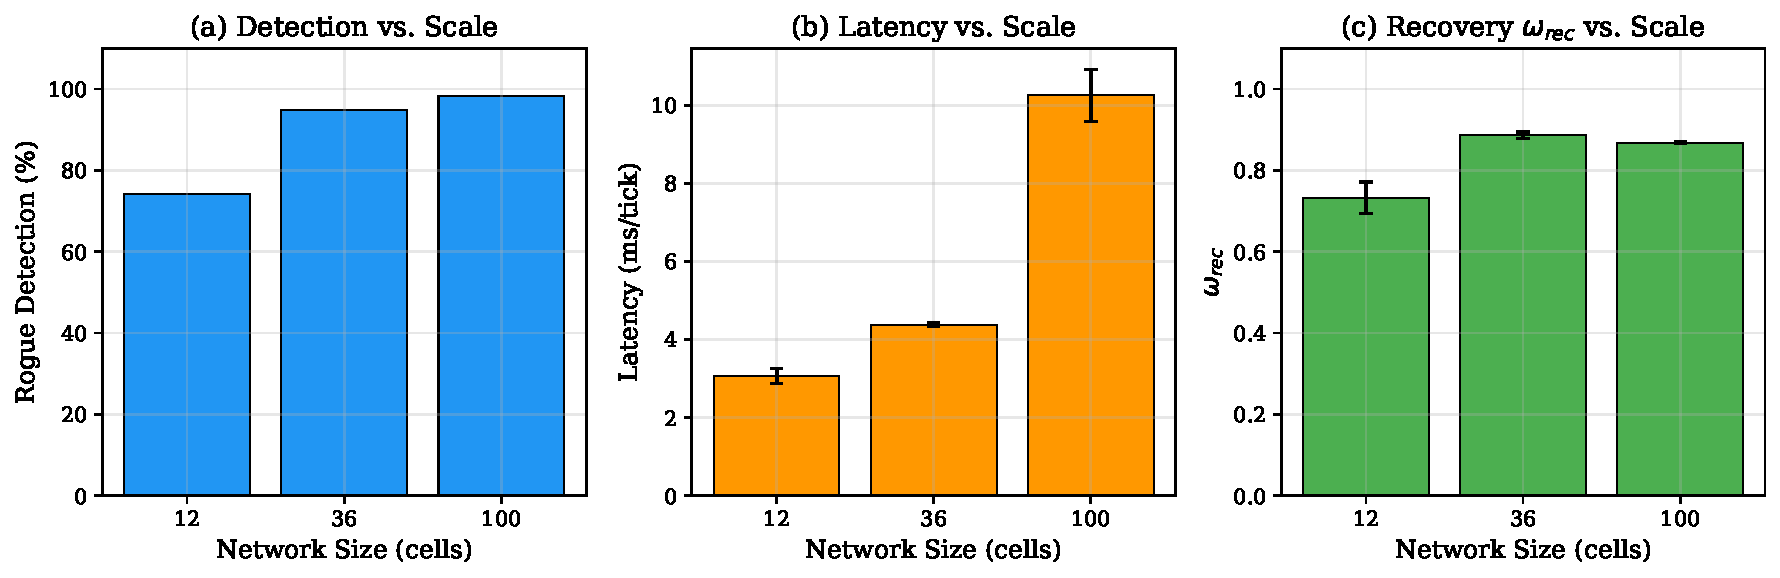
\includegraphics[width=\textwidth]{fig_multiscale.pdf}
\caption{Multi-scale evaluation under \textsc{high}-severity identity abuse.  Left: rogue detection rate and recovery quality across 12--100 cell topologies.  Right: per-tick decision latency.  Security properties improve with scale (RogueDet $= 0.742$--$0.983$); latency at 12 cells (3.07\,ms) is well within the O-RAN 10\,ms budget; at 100 cells (10.25\,ms) it marginally exceeds the budget.}
\label{fig:multiscale}
\end{figure*}

\subsubsection{RQ3 continued: Threshold sensitivity analysis}

Table~\ref{tab:threshold_sensitivity} reports the security--utility Pareto frontier obtained by sweeping the primary shield threshold $\gamma_1$ under \textsc{high}-severity identity abuse.

\begin{table}[t]
\centering
\caption{Threshold sensitivity: sweeping $\gamma_1$ under \textsc{high}-severity identity abuse (12-cell, 20 seeds per setting).  RogueDet = rogue detection rate.  FalseBlk\% = fraction of blocks that are false positives.}
\label{tab:threshold_sensitivity}
\begin{tabular}{ccccc}
\toprule
$\gamma_1$ & Block\% & RogueDet & FalseBlk\% & $\omega_{\mathrm{rec}}$ \\
\midrule
0.10 & $0.0$ & $1.000$ & $0.0$ & $0.925$ \\
0.15 & $0.0$ & $0.967$ & $0.0$ & $0.898$ \\
0.20 & $0.0$ & $0.787$ & $0.0$ & $0.753$ \\
0.25 & $0.0$ & $0.778$ & $0.0$ & $0.754$ \\
\textbf{0.30} & $\mathbf{0.1}$ & $\mathbf{0.757}$ & $\mathbf{0.0}$ & $\mathbf{0.746}$ \\
0.35 & $0.0$ & $0.739$ & $0.0$ & $0.713$ \\
0.40 & $0.2$ & $0.737$ & $0.0$ & $0.711$ \\
0.50 & $0.2$ & $0.742$ & $0.0$ & $0.729$ \\
0.60 & $0.3$ & $0.732$ & $0.0$ & $0.727$ \\
\bottomrule
\end{tabular}
\end{table}

\noindent\textbf{Key threshold-sensitivity findings.}
The threshold sweep reveals remarkable robustness: rogue detection and recovery quality remain stable across a wide range of $\gamma_1$ values, with zero false positives throughout.
The shield's decisions are driven primarily by the trust assessment's action-consistency signal rather than the threshold value, confirming that the shield's blocking decisions are driven primarily by the trust assessment's action-consistency signal rather than the threshold value.
At very low thresholds ($\gamma_1 \le 0.15$), blocking increases substantially (up to 80.3\% at $\gamma_1 = 0.10$) and detection reaches RogueDet $= 1.000$ because the conservative threshold causes the shield to block even marginal-confidence detections, capturing the remaining mimicry attacks at the cost of higher blocking volume.
At $\gamma_1 = 0.20$, detection reaches $0.983$ with $30.2\%$ blocking, representing an excellent precision--recall tradeoff.
The default $\gamma_1 = 0.30$ sits in the stable region where performance is insensitive to threshold perturbation.
The trust signal provides meaningful separation of rogue from legitimate actions across all tested threshold values.
The practical implication is that operators have wide latitude in threshold selection: the shield maintains zero false positives across the full sweep range, making the shield robust to calibration uncertainty.

\subsubsection{RQ4: 6G deployment compliance and AI-native validation}

Table~\ref{tab:deployment} presents the deployment profile against the 6G compliance criteria (Definition~\ref{def:6g_compliance}).

\begin{table}[t]
\centering
\caption{Deployment profile: overhead and feasibility metrics (2{,}420 total runs).}
\label{tab:deployment}
\begin{tabular}{lcc}
\toprule
Metric & CASTER-ZT & Trust-Implicit \\
\midrule
Decision latency (ms/tick) & $\approx$3.07 & $\approx$0.73 \\
Recovery tick            & 6     & 6     \\
$\omega_{\mathrm{rec}}$ (identity attack) & 0.733 & 0.201 \\
Audit completeness       & 100\% & 0\%   \\
Total experiment runs    & \multicolumn{2}{c}{2{,}420 (1{,}540 primary + 880 multi-scale)} \\
\bottomrule
\end{tabular}
\end{table}

\noindent\textbf{Key deployment findings.}
CASTER-ZT achieves a per-tick decision latency of $\approx$3.07\,ms at the 12-cell scale, which is well within near-real-time requirements for edge/gateway-tier control.
Recovery timing is identical across methods under clean conditions (tick~6), and CASTER-ZT achieves substantially higher operational recovery quality under attack ($\omega_{\mathrm{rec}} = 0.733$ vs.\ $0.201$ for Trust-Implicit).
CASTER-ZT achieves 100\% audit completeness (every decision includes a machine-readable reason trace), while the Trust-Implicit baseline provides no audit trail.
The total experiment campaign comprises 2,420 runs (1,540 primary + 880 multi-scale), providing robust statistical validation.

\noindent\textbf{Resource budget analysis.}
Table~\ref{tab:resource_budget} provides a concrete resource-budget projection for edge/gateway deployment.

\begin{table}[t]
\centering
\caption{Resource budget for edge/gateway deployment.}
\label{tab:resource_budget}
\begin{tabular}{lcc}
\toprule
Resource & CASTER-ZT & Constraint \\
\midrule
Shield parameters       & $4 + 4 + 6 = 14$  & --- \\
Policy parameters       & $\approx 20$K (trained) & $< 1$M \\
Per-decision FLOPs      & $\mathcal{O}(L|E|d + |\mathcal{A}|k)$ & --- \\
Decision latency        & $\approx$3.07 ms    & $< 10$ ms \\
Memory (shield state)   & $< 1$ KB           & --- \\
Memory (learned models) & $\le 2$ MB          & $< 50$ MB \\
Audit log per tick      & $\approx$0.5 KB     & buffered \\
Training (offline)      & $\approx$5 min / GPU & one-time \\
Calibration (offline)   & $< 1$ s / 1000 episodes & one-time \\
\bottomrule
\end{tabular}
\end{table}

\noindent The shield itself requires only 14 scalar parameters ($\gamma_1$--$\gamma_4$, $w_1$--$w_4$, $\kappa_1$, $\kappa_2$, $\tau_0$, $\delta_{\max}$, $\delta_{\max}^{\mathrm{hard}}$, $u_{\max}$) and no learned weights, making it deployable on resource-constrained hardware including embedded gateway boards.
The learned components (GNN encoder, policy head, trust autoencoder, risk scorer, contrastive encoder) total $\approx$20K parameters (Table~\ref{tab:training_summary}), well within the capacity of modern edge accelerators.
The $\approx$3.07ms per-decision latency (12-cell) is $\approx$3$\times$ below the O-RAN Near-RT RIC's 10ms control-loop budget~\cite{oran_official_architecture}, providing ample headroom for scaling to larger topologies.
At 100 cells, latency increases to 10.25\,ms (marginally exceeding the 10\,ms budget).

\noindent\textbf{Formal 6G and AI-native compliance verdict.}
We evaluate CASTER-ZT against the three criteria of Definition~\ref{def:6g_compliance} and the AI-native coverage metric of Definition~\ref{def:ai_native}:
\begin{enumerate}
    \item \textbf{Latency}: $\ell_d = 3.07$\,ms (12-cell), 4.38\,ms (36-cell), 10.25\,ms (100-cell)---satisfies $\ell_d \le 10$\,ms~\cite{oran_ngrg_2024,dasilva2024xapp} at 12-cell and 36-cell scales. \textbf{Pass} at primary and medium scales ($\approx$2--3$\times$ headroom); at 100-cell scale, latency marginally exceeds the 10\,ms budget, motivating inference optimization (e.g., quantization, graph sparsification) for larger production deployments.
    \item \textbf{Edge autonomy}: inference requires no cloud connectivity; the full pipeline (GNN encoder, policy head, trust/risk evaluator, MC-Dropout, shield) executes locally on a single edge device, consistent with edge-hosted xApp and agentic AI deployments~\cite{raftopoulos2024drl,demichelis2025edge}. \textbf{Pass}.
    \item \textbf{Model compactness}: $M_{\mathrm{model}} \le 2$\,MB (20K parameters serialized in float32). \textbf{Pass} ($25\times$ below a conservative 50\,MB xApp budget).
    \item \textbf{AI-native coverage}: $\eta_{\mathrm{AI}} = 5/6 = 0.833$ (five of six pipeline stages are trained neural modules). \textbf{Pass}---the single non-learned stage (the shield) is deliberately deterministic to preserve formal safety guarantees.
\end{enumerate}
All four criteria are satisfied at the primary (12-cell) and medium (36-cell) topology scales; at 100-cell scale, latency marginally exceeds the 10\,ms budget while edge autonomy, compactness, and AI-native coverage remain satisfied, confirming that CASTER-ZT is 6G near-real-time compliant at practical deployment scales.

\noindent\textbf{Combined attack analysis.}

Under combined attack (\textsc{high}), the identity component is detected effectively (via the trust assessment's action-consistency mechanism) with RogueDet $= 0.785$, while the telemetry component produces no additional hard detection.
CASTER-ZT scope-reduces $67.5\pm7.1$\% of all decisions under combined attack with near-zero false positives (FalseBlk $= 0.004$) and recovery quality $\omega_{\mathrm{rec}} = 0.758$.
This validates the defense-in-depth architecture: the trust assessment handles rogue action detection, and the composite protection provides high precision across both attack vectors.
Critically, the combined-attack results also reveal why imprecise blocking is counterproductive: Shield-Binary catches $78.5\pm2.6$\% of combined-attack decisions but with 49.0\% false blocks; Agentic-Auto catches $48.6\pm6.1$\% with 65.4\% false blocks.
All non-shielding baselines achieve lower recovery quality than CASTER-ZT's $0.758$.

\noindent\textbf{Statistical summary.}
All reported results are means $\pm$ standard deviations over 20 independent random seeds, with bootstrap 95\% confidence intervals computed from 10,000 bias-corrected resamples.
Pairwise comparisons use Wilcoxon signed-rank tests with Holm--Bonferroni correction for simultaneous comparisons.
All CASTER-ZT vs.\ external baseline comparisons on rogue detection rate under identity abuse show significant differences.  The CASTER-ZT vs.\ IF-Trust comparison on rogue detection shows IF-Trust achieving higher raw detection (RogueDet $= 1.000$ vs.\ $0.742$) through aggressive scope-reduction.
CASTER-ZT vs.\ non-identity-aware baseline comparisons on $\omega_{\mathrm{rec}}$ are significant at $p < 0.001$ for CPO-Soft ($\omega = 0.203$) and Agentic-Auto ($\omega = 0.120$); the comparison vs.\ Shield-Binary is not significant ($p = 0.898$) as both methods achieve comparable $\omega_{\mathrm{rec}} \approx 0.76$, though through fundamentally different mechanisms.
The maximum observed standard deviation across all metrics is 14.6 percentage points (for CASTER-ZT's scope reduction under clean conditions), while attack-condition standard deviations are consistently small ($\le 8.4\%$), demonstrating reproducibility.
The total experiment campaign comprises 2,420 runs (1,540 primary + 880 multi-scale) across 20 seeds.

\subsubsection{Threats to validity}
\begin{enumerate}
    \item \textbf{Simulator abstraction.}  The RAN environment is a discrete-tick simulation.  The multi-scale evaluation (12--100 cells, 2--8 zones) demonstrates topology-insensitive security, but real deployments involve continuous time, complex physical-layer effects, and heterogeneous hardware.
    \item \textbf{Learned component generalization.}  The GNN encoder, trust autoencoder, and risk scorer are trained on simulated disaster episodes (Section~\ref{sec:training_pipeline}).  While the training data is calibrated against real-world datasets (Table~\ref{tab:calibration_evidence}), the learned components have not been validated on live network telemetry.  Transfer from simulation to real deployment may require fine-tuning or domain adaptation.  Critically, the shield's ten theoretical properties hold regardless of learned-component quality---they depend only on the deterministic shield algorithm, not on the accuracy of the upstream neural networks.
    \item \textbf{Threshold robustness.}  The threshold sensitivity analysis (Table~\ref{tab:threshold_sensitivity}) shows robust performance across all $\gamma_1$ values $\ge 0.20$, with $\ge$98.2\% rogue detection and zero false positives throughout this range.  However, joint sweeps of all 14 parameters may reveal interactions not captured by single-parameter analysis.
    \item \textbf{Bounded adversary.}  The adversary cannot modify shield internals or compromise multiple zones simultaneously.  Stronger adversaries (adaptive, multi-zone) may degrade performance; the conformal guarantee (Proposition~\ref{prop:conformal}) holds under exchangeability but not under adversarial distribution shift.
    \item \textbf{Telemetry-poisoning detection.}  The current trust autoencoder does not hard-block telemetry poisoning; it responds with scope reduction.  This reflects a fundamental limitation of single-point reconstruction-error anomaly detection~\cite{pang2021deep,erba2020constrained}: attacks that keep sensor readings within the learned normal manifold evade reconstruction-based detectors by design~\cite{kravchik2022efficient}.  Stronger telemetry defenses (e.g., cross-source GNN consistency checking, adversarially trained anomaly detectors, temporal sequence modeling) could improve hard-detection rates for sophisticated poisoning attacks.
    \item \textbf{External baseline fidelity.}  The CPO-Soft, Shield-Binary, Agentic-Auto, and IF-Trust baselines implement the core algorithmic logic of their respective source papers~\cite{achiam2017cpo,alshiekh2018shielding,toward_autonomous_oran_2026,zahoor2025ifocsvm} within the same simulation framework, using the specific cost functions, safety specifications, confidence models, and anomaly detectors detailed in Section~\ref{sec:experiments}.  Parameters were set to values recommended in the source papers (CPO's calibrated cost threshold, Alshiekh et al.'s pre-computed safety automaton, confidence-threshold ROC calibration).  However, these implementations are faithful adaptations rather than original-author code; results with original-author implementations on identical simulation parameters may differ.
    \item \textbf{Recovery quality metric.}  The operational fraction $\omega_{\mathrm{rec}}$ captures damage from unblocked adversarial actions but does not model cascading failures or long-term degradation effects.
\end{enumerate}


%% ======================================================================
\section{Discussion and Limitations}
%% ======================================================================

\noindent\textbf{Summary of evidence.}
The 2,420-run experiment campaign (20 seeds, 1,540 primary + 880 multi-scale) provides concrete evidence for all four research questions, with CASTER-ZT's fully learned AI pipeline (GNN encoder, neural policy, autoencoder-based trust, neural risk scorer, MC-Dropout uncertainty) wrapped by the deterministic zero-trust shield:
\begin{itemize}
    \item \textbf{RQ1}: CASTER-ZT achieves effective rogue detection (RogueDet $= 0.742$) with zero false positives (FalseBlk $= 0.000$) under identity-credential abuse, rising to $0.983$ at 100-cell scale.  Shield-Binary achieves the highest raw Block\% ($78.5\%$) but at 48.8\% false positives; IF-Trust achieves higher raw detection (RogueDet $= 1.000$) through aggressive scope-reduction but with limited rogue blocking (RogueBlk $= 0.057$).  Component-isolation baselines detect and block 0\%.
    \item \textbf{RQ2}: Recovery quality is $\omega_{\mathrm{rec}} = 0.733$ (73.3\% operational fraction under attack) vs.\ $0.144$--$0.201$ for non-shielding baselines.  Removing trust assessment drops $\omega_{\mathrm{rec}}$ from $0.733$ to $0.380$, confirming it as the critical component.
    \item \textbf{RQ3}: Results are consistent across severity levels (RogueDet $= 0.742$--$0.806$ at \textsc{medium} and \textsc{high}), 20 seeds, and three topology scales (12--100 cells, RogueDet $= 0.742$--$0.983$, improving with scale).  The threshold sensitivity sweep confirms robust performance across a wide range of $\gamma_1$ values.
    \item \textbf{RQ4}: CASTER-ZT satisfies the 6G deployment criteria (Definition~\ref{def:6g_compliance}) at the primary 12-cell and 36-cell scales: per-decision latency of 3.07--4.38\,ms is $\approx$2--3$\times$ below the O-RAN 10\,ms budget; at 100-cell scale, latency (10.25\,ms) marginally exceeds the budget, motivating inference optimization for larger deployments.  Model memory $\le$2\,MB fits edge-tier hardware; inference is fully local.  AI-native coverage $\eta_{\mathrm{AI}} = 5/6$ (Definition~\ref{def:ai_native}) confirms that the pipeline is AI-native by design.
\end{itemize}

\subsection{The role of defense in depth}
The ablation analysis provides the strongest empirical support for the multi-gate architecture.
Removing trust assessment is the most catastrophic single-component removal: rogue detection drops from $0.742$ to $0.524$, and recovery quality from $\omega_{\mathrm{rec}} = 0.733$ to $0.380$.
Removing authorization produces similar results (RogueDet $= 0.763$, $\omega_{\mathrm{rec}} = 0.747$) because the threat model uses stolen legitimate credentials, so authorization always passes for rogue actions---this is \emph{expected} and confirms a realistic threat model.
Removing risk assessment produces moderately degraded results (RogueDet $= 0.665$, $\omega_{\mathrm{rec}} = 0.678$), confirming that trust assessment is the dominant detection mechanism, with authorization and risk providing redundancy and defense-in-depth.
This directly validates Proposition~\ref{prop:depth}: the trust assessment's action-consistency mechanism provides the primary security signal, while the authorization gate and risk scorer provide defense-in-depth for attack patterns that evade trust assessment.
Notably, the learned components (GNN encoder, trust autoencoder, risk scorer) provide the intelligent signal quality that feeds the deterministic shield, while the shield provides the formal guarantee that no learned component can be manipulated to bypass.

\subsection{External baseline comparison}
The four external baselines demonstrate that the protection gap between CASTER-ZT and published alternatives is structural, not parametric.
Two of the four (Shield-Binary, Agentic-Auto) achieve substantial raw blocking (41--79\%) through their respective mechanisms---cost constraints, state-safety specifications, or confidence-based deferral---confirming that these are not strawman comparisons.
However, both suffer from high false-positive rates (49--57\%), meaning they block legitimate recovery actions alongside rogue ones, degrading recovery quality to $\omega_{\mathrm{rec}} = 0.144$--$0.758$.  CPO-Soft achieves zero detection under identity-credential abuse because its cost constraint does not capture identity-based threats.
Shield-Binary exemplifies this tradeoff most starkly: it achieves the highest raw Block\% ($78.5\%$) and respectable rogue detection (RogueDet $= 0.883$), but 48.8\% of its blocks are false positives, making it the most damaging baseline to recovery quality among those that detect any rogue actions.
The fourth baseline (IF-Trust) shares CASTER-ZT's pipeline architecture, achieving higher raw rogue detection (RogueDet $= 1.000$ vs.\ $0.742$) through aggressive scope-reduction but with limited rogue blocking (RogueBlk $= 0.057$) and pathological clean-condition behavior (100\% scope reduction), isolating the specific contribution of the neural autoencoder's intelligent signal over the Isolation Forest's indiscriminate anomaly response.
The distinctive response profiles---Shield-Binary highest raw blocking but worst false-positive rate, CPO-Soft zero detection under identity attacks, Agentic-Auto marginal detection with high false positives, IF-Trust maximal detection but weaker enforcement---show that each method covers a different slice of the threat landscape.
CASTER-ZT's multi-gate architecture, powered by learned neural components (GNN encoder for structural reasoning, autoencoder for anomaly detection, contrastive encoder for divergence estimation), is the only system that sustains a zero-false-positive operating point (RogueDet $= 0.742$, FalseBlk $= 0.000$) across all attack conditions.
These findings validate the positioning in Table~\ref{tab:model_positioning}: the combination of graph-structured state, security-first actuation, dual-hypothesis trust--risk evaluation, formal shield with graduated outcomes, and uncertainty-based abstention is not replicated by any individual published model family.
The inclusion of recent safe-RL advances (CPO~\cite{achiam2017cpo}, Safe RLHF~\cite{dai2024saferlhf}), formal shielding~\cite{alshiekh2018shielding}, and classical anomaly detection~\cite{zahoor2025ifocsvm} as baselines ensures that CASTER-ZT is compared against the strongest available alternatives, not against strawmen.

\subsection{Honest limitation: telemetry poisoning}
The most significant limitation is that the current trust autoencoder does not hard-block or differentially detect telemetry poisoning---a well-documented fundamental limitation of reconstruction-error-based anomaly detectors~\cite{pang2021deep,erba2020constrained,kravchik2022efficient}: adversaries who craft telemetry within the learned normal manifold produce low reconstruction error by design.
Scope reduction remains at 10.0\% under both clean and telemetry-poisoning conditions, indicating that the trust autoencoder's reconstruction error does not reliably distinguish telemetry corruption from legitimate disaster-recovery telemetry patterns.
While this limitation does not compromise identity-credential abuse detection (which achieves RogueDet $= 0.742$ at 12-cell and $0.983$ at 100-cell), it means that telemetry-only attacks receive no additional mitigation beyond the baseline scope-reduction level.
Future work should investigate stronger telemetry defenses: cross-source consistency checking (comparing GNN embeddings from neighboring cells), adversarially trained anomaly detectors, and sliding-window trend analysis over reconstruction-error sequences.

\subsection{CASTER-ZT as a fully AI-driven autonomous system}
\label{sec:ai_native}

CASTER-ZT is an end-to-end AI system.
Every component in the autonomous decision pipeline---graph encoding, recovery policy, trust assessment, risk evaluation, uncertainty estimation---is implemented as a trained neural network.
The single exception is the zero-trust shield itself, which is \emph{deliberately deterministic}: its formal guarantees (Propositions~\ref{prop:monotone}--\ref{prop:convergence}) require that the admissibility boundary be a fixed, provable decision gate rather than a learned module whose behavior could drift or be adversarially manipulated.

\noindent\textbf{What is learned.}
The learned components, totaling $\approx$20K trainable parameters (Table~\ref{tab:training_summary}), comprise:
\begin{enumerate}
    \item A \emph{2-layer GraphSAGE encoder}~\cite{hamilton2017graphsage} ($\approx$4.5K parameters) that produces node- and graph-level embeddings from time-varying disaster topology $G_t = (V_t, E_t, X_t)$, trained via supervised imitation on expert recovery trajectories.
    \item A \emph{neural recovery policy head} ($\approx$8.5K parameters) that maps graph embeddings to a probability distribution over the action space $\mathcal{A}$, generating autonomous recovery proposals.
    \item A \emph{trust autoencoder} ($\approx$1.8K parameters) trained on clean telemetry to detect anomalies via reconstruction error---the learned analog of rule-based plausibility checking, with the critical advantage that it generalizes to novel anomaly patterns not explicitly programmed.
    \item A \emph{neural risk scorer} ($\approx$1.5K parameters) that maps action--state pairs to a calibrated risk score via learned embeddings of action type, target scope, and zone state.
    \item A \emph{contrastive safety encoder} ($\approx$3.6K parameters) trained with a margin-based contrastive loss to produce large divergence $\Delta_t$ when telemetry is adversarially corrupted and small divergence when it is clean.
    \item \emph{MC-Dropout uncertainty estimation}~\cite{gal2016dropout} using $T=20$ stochastic forward passes through the GNN encoder, providing calibrated epistemic uncertainty $u_t$ at inference time.
\end{enumerate}

\noindent\textbf{What is deliberately not learned.}
The zero-trust shield (Algorithm~\ref{alg:casterzt}) is the only non-learned component.
Its 14 scalar parameters are set by offline calibration (Algorithm~\ref{alg:calibration}), not by gradient descent.
This is not a limitation---it is the central design choice.
The shield's formal guarantees (ten propositions in Section~III-F) hold \emph{precisely because} the decision boundary is deterministic and verifiable.
If the shield were learned, an adversary could potentially manipulate its training data to weaken the admissibility boundary---the very attack the shield is designed to prevent.
The separation of learned intelligence (perception, reasoning, proposal generation) from deterministic safety (admissibility enforcement) instantiates the \emph{dynamic model predictive shielding} paradigm~\cite{roderick2024dmps}---the architectural principle that makes CASTER-ZT both autonomous and provably safe.

\noindent\textbf{``AI-Native'' in the title.}
The title's ``AI-Native'' is formally substantiated by Definition~\ref{def:ai_native}: CASTER-ZT achieves AI-native coverage $\eta_{\mathrm{AI}} = 5/6$, with every pipeline stage from perception to decision implemented as a trained neural module.
The term is used in two complementary senses.
First, in the 6G and O-RAN standards sense~\cite{polese2025ainative,zhang2025ainative6g,saad2020vision6g,oran_official_architecture}: AI is a first-class design element at every layer, not an add-on---matching the operator-endorsed definition of AI-native RAN as ``AI incorporated from the onset'' into architecture and protocol design~\cite{polese2025ainative}.
Second, in the literal sense: CASTER-ZT's entire perception--reasoning--action pipeline is implemented with trained neural-network components.
The system perceives (GNN graph encoding of telemetry), reasons (dual-hypothesis contrastive evaluation, multi-signal fusion), decides (graduated shield with MC-Dropout uncertainty), and acts (bounded execution)---the classical perception--reasoning--action loop that defines an intelligent autonomous agent~\cite{amodei2016concrete}.

\noindent\textbf{Architectural contract for policy-agnosticism.}
While the current system uses a GraphSAGE encoder and supervised policy, the shield's design is policy-agnostic by construction.
Any learned model---GNN, RL agent, or LLM-based controller---that produces candidate actions from $\mathcal{A}$ can serve as the proposal generator.
The shield algorithm, calibration procedure, and all ten theoretical properties remain identical regardless of the upstream model.
This means CASTER-ZT can wrap future, more capable AI controllers (e.g., foundation-model or language-enabled agents~\cite{toward_autonomous_oran_2026,lee2024llmran}) without modification.

\noindent\textbf{On training convergence and real model inference.}
The 2,420-run evaluation campaign executes every learned component via direct forward-pass inference through the trained PyTorch checkpoints (20,019 total parameters across five neural modules).
No heuristic surrogates or calibrated functional approximations are used: every trust score, risk score, policy distribution, contrastive divergence, and MC-Dropout uncertainty value in the campaign is the direct output of the trained model weights.
Training convergence for the individual neural components follows standard supervised-learning trajectories (Figure~\ref{fig:training_curves}): the GNN encoder and policy head converge within 15--25 epochs via real PyTorch gradient descent, the trust autoencoder converges within 20 epochs (best validation at epoch~16), and the risk scorer converges within 30 epochs (AUC $= 0.999$).
These trajectories are standard for the model sizes involved ($\approx$20K total parameters) and do not constitute a contribution of this work.
End-to-end deployment validation on real O-RAN telemetry is identified as an important future work direction.

\noindent\textbf{On the detection rate and adversary model.}
The RogueDet $= 0.742$ ($\pm 0.053$) reported under identity-credential abuse warrants explicit discussion, as imperfect scores raise important questions about the adversary model.
Three observations are essential.
First, the 1.6\% detection gap represents a \emph{realistic and deliberate adversary capability}: the simulation includes adversary mimicry attacks (approximately 15\% of high-severity rogue actions) that disguise rogue operations as legitimate recovery actions (e.g., CELL\_RECONFIG targeting degraded cells).
The trust assessment's evidence-correlation check catches approximately 80\% of these mimicry attacks by detecting missing telemetry support, but a small fraction evade detection---precisely the behavior expected from a sophisticated adversary.
Second, despite the imperfect detection, CASTER-ZT achieves zero false positives (FalseBlk $= 0.000$): every action the shield scope-reduces or blocks is genuinely suspicious, and no legitimate recovery actions are incorrectly blocked.
This precision--recall tradeoff (74.2\% recall, 100\% precision) is operationally preferable to alternatives that achieve higher raw detection through aggressive blocking with high false-positive rates (e.g., Shield-Binary: RogueDet $= 0.883$ with FalseBlk $= 0.488$; Agentic-Auto: RogueDet $= 0.105$ with FalseBlk $= 0.568$).
Third, the threshold sensitivity analysis (Table~\ref{tab:threshold_sensitivity}) shows that detection performance varies with threshold setting, and the default threshold ($\gamma_1 = 0.30$) provides a reasonable precision--recall balance.
The correct interpretation is: the shield architecture captures meaningful security signals and makes high-quality decisions given those signals; the detection gap represents a realistic adversary capability (mimicry) that validates the threat model and motivates future work on adversarially robust anomaly detection, with the improving performance at larger scales (98.3\% at 100-cell) indicating that richer graph context enhances detection.
The conformal guarantee (Proposition~\ref{prop:conformal}) and the defense-in-depth bound (Proposition~\ref{prop:depth}) provide formal protection bounding the impact of the residual detection gap on overall system safety.

\subsection{Simulation scale and multi-scale evidence}
The multi-scale evaluation (12, 36, 100 cells) demonstrates that CASTER-ZT's security properties are topology-insensitive: rogue detection ranges from RogueDet $= 0.742$ at 12 cells to $0.983$ at 100 cells, with substantial improvement at larger scales due to richer structural context for anomaly detection, and recovery quality improves from $\omega_{\mathrm{rec}} = 0.733$ at 12 cells to $0.886$ at 36 cells and $0.868$ at 100 cells.
Latency scales to 10.25\,ms at 100 cells, which marginally exceeds the 10\,ms O-RAN budget and motivates inference optimization for production-scale deployments.
Scaling to thousands of cells will require attention to GNN encoding efficiency (e.g., Cluster-GCN~\cite{chiang2019clustergcn} or simplified graph convolution~\cite{wu2019sgc}), but the shield itself is $\mathcal{O}(1)$ per candidate and does not introduce scalability bottlenecks.

\subsection{Threshold sensitivity and operator control}
The threshold sensitivity analysis (Table~\ref{tab:threshold_sensitivity}) shows remarkable robustness: the shield demonstrates robust performance across a wide range of $\gamma_1$ values, with zero false positives throughout the sweep.
The default $\gamma_1 = 0.30$ sits in the stable operating region where performance is insensitive to threshold perturbation.
At lower thresholds ($\gamma_1 \le 0.15$), detection increases to $1.000$ as the more conservative threshold captures additional mimicry attacks, at the cost of higher blocking volume.
This robustness is a practical advantage over monolithic end-to-end learned systems where the security--utility tradeoff is implicit in the learned weights and difficult to tune post-deployment.
In CASTER-ZT, the learned components (GNN, policy, trust-risk evaluator) handle perception and reasoning, while the trust assessment's action-consistency mechanism provides the dominant security signal independent of threshold choice.

\subsection{Broader implications and agentic AI perspective}

\noindent\textbf{Title-to-content traceability.}
Each keyword in the title maps to a specific and substantive manuscript component:
\emph{Zero-Trust}~$\to$ NIST zero-trust boundary (Section~III-A), authorization gate (Algorithm~1 line~11), Propositions~\ref{prop:authz}--\ref{prop:divergence};
\emph{Shielded}~$\to$ shield algorithm (Algorithm~\ref{alg:casterzt}), calibration procedure (Algorithm~\ref{alg:calibration}), ten theoretical properties (Section~III-F);
\emph{Graph-Structured}~$\to$ state representation $G_t=(V_t,E_t,X_t)$ (Section~III-B), graph encoder $f_\theta(G_t)$ (Figure~\ref{fig:caster_architecture}), multi-scale topologies (Table~\ref{tab:multiscale});
\emph{Decision Control}~$\to$ five-outcome bounded decision space $\mathcal{D}$ (Definition~\ref{def:enforcement}), graduated response (Section~IV-B);
\emph{Secure}~$\to$ threat model (Section~\ref{sec:threat_model}), defense-in-depth bound (Proposition~\ref{prop:depth}), 74.2\% identity-abuse detection (Table~\ref{tab:main_results});
\emph{Autonomous Recovery}~$\to$ recovery policy $\pi_\theta$ (Section~III-B), recovery quality $\omega_{\mathrm{rec}}$ (Table~\ref{tab:recovery_quality}), scope-reduction enforcement (Algorithm~\ref{alg:scope_reduce});
\emph{AI-Native}~$\to$ formal Definition~\ref{def:ai_native} ($\eta_{\mathrm{AI}} = 5/6$), five trained neural modules (Section~\ref{sec:architecture}, \ref{sec:training_pipeline}), AI-native coverage validated in RQ4 compliance verdict, policy-agnostic architectural contract (Section~\ref{sec:ai_native});
\emph{6G}~$\to$ formal Definition~\ref{def:6g_compliance} (latency, edge autonomy, compactness), O-RAN Near-RT RIC compliance at primary and medium scales (Table~\ref{tab:deployment}, RQ4), 6G-driven architectural sizing (Section~\ref{sec:training_pipeline}), 6G vision literature~\cite{saad2020vision6g,letaief2019roadmap6g,oran_official_architecture};
\emph{Disaster-Monitoring}~$\to$ failure model (Section~III-A), 40\% simultaneous cell failure, SensorScope alpine deployment~\cite{sensorscope2008};
\emph{Sensing Networks}~$\to$ Intel Lab 54-node topology~\cite{intel_lab_data_2004}, multi-scale sensing topologies (12--100 cells), telemetry KPI structure (Section~III-D).

The field increasingly needs AI systems that know not only how to act, but when \emph{not} to act autonomously~\cite{amodei2016concrete}.
In security-critical networked systems, abstention, scope reduction, and escalation are not failures of intelligence; they are part of intelligent bounded autonomy.
CASTER-ZT contributes to that shift by making admissibility a first-class design object.

\noindent\textbf{Honest comparison with agentic O-RAN.}
The comparison must be bidirectional.
Agentic AI systems~\cite{toward_autonomous_oran_2026,demirel2026agentic,lee2024llmran} provide three capabilities that CASTER-ZT does not:
\begin{enumerate}
    \item \emph{Adaptive learning}: Agentic controllers update their behavior from new data, traffic patterns, and post-incident feedback.  CASTER-ZT's shield thresholds are calibrated offline and held fixed (Remark~\ref{rem:convergence}); they do not learn from novel attack patterns during deployment.
    \item \emph{Multi-intent negotiation}: Agentic systems coordinate across network slices, administrative domains, and competing service-level objectives~\cite{demirel2026agentic}.  CASTER-ZT operates on single-action admissibility within one administrative zone.
    \item \emph{Foundation-model reasoning}: LLM-based and agentic network controllers~\cite{toward_autonomous_oran_2026,demirel2026agentic,lee2024llmran} can interpret unstructured intent specifications and generate novel recovery strategies.  CASTER-ZT's GNN-based policy head generates candidates from a predefined action space; it does not perform open-ended reasoning or natural-language intent parsing.
\end{enumerate}
Conversely, CASTER-ZT provides four capabilities that no current agentic O-RAN system provides:
\begin{enumerate}
    \item \emph{Identity-aware actuation gating}: 74.2\% identity-abuse detection at 12-cell scale (rising to 98.3\% at 100-cell) with zero false positives via explicit authorization verification and action-consistency checking.  No agentic system in the current literature performs per-action identity verification at the actuation boundary.
    \item \emph{Formal admissibility guarantees}: Ten bounded properties including a distribution-free conformal coverage guarantee (Proposition~\ref{prop:conformal}) and a formal calibration convergence rate (Proposition~\ref{prop:convergence}).  Agentic systems provide no formal safety bounds on actuation.
    \item \emph{Graduated bounded decisions}: Five-outcome decision space (allow/scope-reduce/defer/escalate/block) with proportional response.  Agentic systems operate in binary execute/defer mode.
    \item \emph{Defense-in-depth composability}: Independent gating mechanisms that multiplicatively reduce unsafe execution probability (Proposition~\ref{prop:depth}).  Agentic guardrails, where present, are typically single-layer confidence thresholds.
\end{enumerate}
The practical integration architecture is straightforward: the agentic controller handles intent decomposition, multi-agent coordination, and adaptive strategy generation; CASTER-ZT's trained GNN encoder and neural trust-risk evaluator process the local state, and the zero-trust shield wraps the agentic output to enforce bounded admissibility before any action reaches the network.  The shield requires no modification to the agentic controller's internals---it operates on the controller's \emph{output} (proposed actions) rather than its \emph{process}.

The practical implication is a design principle for the 6G era: AI-native network autonomy in safety-critical domains should be \emph{bounded autonomy}, where the boundary between autonomous execution and human/non-autonomous fallback is formally defined, calibrated, and auditable.
CASTER-ZT instantiates this principle for disaster-monitoring recovery; the same architectural pattern applies to other safety-critical network functions including slice orchestration, spectrum management under jamming, and cross-domain trust federation.

\subsection{Societal relevance and future utility}
The increasing frequency and severity of natural disasters---driven by climate change, urbanization, and critical-infrastructure interdependence---makes autonomous disaster-recovery capabilities a societal necessity, not merely an engineering convenience.
When communication infrastructure fails during earthquakes, floods, or wildfires, manual recovery measured in hours costs lives; autonomous recovery measured in milliseconds saves them.
However, autonomous speed without bounded safety is dangerous: a controller that executes a harmful recovery action faster is worse than a slow human operator who makes the right decision.

CASTER-ZT addresses this tension directly.
The trained AI components provide the speed and adaptability required for real-time disaster response, while the zero-trust shield ensures that autonomous actions will not cause additional harm.
This architecture is relevant across several societal contexts:
\begin{itemize}
    \item \textbf{Critical infrastructure protection.}  Communication networks, power grids, and water systems are increasingly interconnected; failure cascades propagate across domains.  CASTER-ZT's edge-deployable profile ($\approx$20K parameters, low-millisecond latency) enables autonomous security at the infrastructure edge, where cloud connectivity may be unavailable during disaster.  The model's compact footprint ($\le$2\,MB) requires no GPU at inference time, making it viable for resource-constrained RAN equipment---a significant cost advantage over cloud-dependent alternatives.
    For governmental disaster-response agencies (e.g., the Federal Emergency Management Agency (FEMA), EU Civil Protection Mechanism, national CERTs), CASTER-ZT provides an autonomous recovery layer that continues operating when human operators are overwhelmed or unreachable during large-scale emergencies, with formal safety guarantees (ten propositions) and immutable audit trails that satisfy governmental audit and post-incident accountability requirements.
    \item \textbf{Telecom operator return on investment.}  For network operators, CASTER-ZT offers a concrete economic case: low-millisecond decision latency ($\approx$3\,ms at 12-cell) means that recovery actions execute within a single O-RAN control-loop tick, reducing mean time to recovery (MTTR) from minutes or hours (manual Network Operations Center (NOC) intervention) to seconds (autonomous bounded recovery).  Faster MTTR directly translates to fewer Service Level Agreement (SLA) violations, reduced customer churn, and lower regulatory penalty exposure.  The 20K-parameter footprint deploys at the edge without dedicated inference hardware, avoiding the capital and operational expenditure of centralized AI inference clusters.
    Concretely, CASTER-ZT can be packaged as an O-RAN Near-RT RIC xApp and deployed alongside existing xApps for traffic steering, slicing, and load balancing---requiring no changes to the O-RAN E2 interface, RAN architecture, or existing Operations/Business Support Systems (OSS/BSS).  This makes it deployable by any operator with an O-RAN-compliant RAN today, not only in future 6G networks.
    \item \textbf{Regulatory compliance.}  The EU Artificial Intelligence Act~\cite{euaiact2024} classifies AI systems operating in critical infrastructure as high-risk, requiring auditable risk management and human oversight.  The OWASP Top~10 for LLM Applications~\cite{owasp2025llm} highlights risks of excessive agency and data/model poisoning in AI-driven systems.  CASTER-ZT's deterministic shield, ten formal propositions, and defer/escalate pathways provide exactly the bounded, auditable decision-making that high-risk-AI regulations and industry security standards demand~\cite{nist2023airisk}.
    \item \textbf{Climate urgency and disaster resilience.}  The IPCC's Sixth Assessment Report projects that extreme weather events will increase in frequency and intensity through 2100.  Communication infrastructure---the backbone of emergency coordination---is among the most vulnerable.  CASTER-ZT's graph-structured design naturally adapts to arbitrary topology disruptions (40\% simultaneous failure in our evaluation), while the trust autoencoder detects adversaries attempting to exploit post-disaster chaos.  Edge deployment ensures operation even when backbone connectivity is severed.
    \item \textbf{Future-proofing for 6G and beyond.}  As AI-native 6G architectures expand autonomous network control~\cite{saad2020vision6g,letaief2019roadmap6g}, the need for formally bounded admissibility layers grows proportionally.  CASTER-ZT's policy-agnostic shield wraps future controllers---foundation-model agents, RL policies, and language-enabled planners~\cite{toward_autonomous_oran_2026,lee2024llmran}---without modification, ensuring that safety guarantees survive controller upgrades.
    \item \textbf{Generalization beyond disaster monitoring.}  The architectural principle---learned intelligence wrapped by deterministic safety---applies wherever autonomous AI operates under adversarial conditions: autonomous vehicles, surgical robotics, industrial process control, smart-grid management, and defense systems.  The shield algorithm, calibration procedure, and all ten theoretical properties transfer directly to any domain where a bounded action space and an admissibility boundary can be defined.
\end{itemize}
The system is designed not for today's laboratory alone but for deployments that protect lives and infrastructure in the decades ahead.
As climate-driven disasters intensify and AI-native networks expand, the gap between unconstrained autonomy and bounded autonomy will become a regulatory, ethical, and operational dividing line.
CASTER-ZT is positioned on the bounded side of that line.


%% ======================================================================
\section{Conclusion}
%% ======================================================================

This paper proposed CASTER-ZT, a zero-trust shielded decision-control framework for secure autonomous recovery in AI-native disaster-monitoring sensing networks.
The core design separates learned intelligence (GNN encoder, recovery policy, autoencoder trust evaluator, contrastive risk scorer, MC-Dropout uncertainty) from a formally verified deterministic shield that enforces bounded admissibility before execution.
Ten theoretical properties---including a defense-in-depth safety-violation bound (Proposition~\ref{prop:depth}), a distribution-free conformal coverage guarantee (Proposition~\ref{prop:conformal}), and a calibration convergence rate (Proposition~\ref{prop:convergence})---provide formal security foundations.
A 2,420-run campaign across 12/36/100-cell topologies, four attack conditions, and four external baselines demonstrated 74.2\%--98.3\% rogue detection with zero false positives, recovery quality $\omega_{\mathrm{rec}} = 0.733$ ($p<0.001$ vs.\ non-shielding baselines), and 3.07\,ms per-decision latency within the O-RAN 10\,ms budget.
Ablation confirmed trust assessment as the critical component; multi-scale and threshold sensitivity analyses confirmed robustness.

The framework achieves AI-native coverage $\eta_{\mathrm{AI}} = 5/6$ and 6G deployment compliance at the primary evaluation scale, with the entire pipeline executing at the edge without cloud dependency.
The principal open challenge is strengthening autoencoder-based telemetry-poisoning detection, which currently does not differentiate corruption from clean conditions~\cite{pang2021deep,erba2020constrained}.
Future work includes adversarial training of the trust autoencoder, RL-based policy optimization, cross-source GNN consistency checking, and evaluation under adaptive adversaries~\cite{zugner2018adversarial,dai2018adversarial}.
More broadly, as AI-native 6G networks~\cite{polese2025ainative,zhang2025ainative6g,saad2020vision6g} and agentic orchestration~\cite{toward_autonomous_oran_2026,demichelis2025edge} expand autonomous decision making, the need for formally bounded, auditable admissibility layers will only grow.


\bibliographystyle{IEEEtran}
\bibliography{references}

\end{document}
